\documentclass[11pt]{article}
\usepackage{debulletin,times,epsfig,subfigure,wrapfig,algorithmic,color,boxedminipage,graphicx,url}

% this is the template for an issue of the Data Engineering Bulletin

% all packages used by any paper must be listed here
\usepackage{subfig}
\usepackage{listings}
\usepackage{caption}
\usepackage{microtype}
\usepackage{listings}
\usepackage{booktabs}
\usepackage{listings}
\usepackage{xargs}
%\PassOptionsToPackage{hyphens}{url}
%\usepackage{hyperref}
\usepackage{multirow}
\usepackage{tabularx}
\usepackage{makecell}
\usepackage{arydshln}
\usepackage{xspace}
\usepackage{tcolorbox}
\usepackage{xpatch}

\newcommand{\Hypercallback}{Hyperupcall\xspace{}}
\newcommand{\hypercallback}{hyperupcall\xspace{}}
\newcommand{\hide}[1]{}

\begin{document}


% please enter real date, vol no, issue no
\bulletindate{September 2019}
\bulletinvolume{42}
\bulletinnumber{3}
\bulletinyear{2019}

% these are files that I have- but your part of the issue can be done without
% them
\IEEElogo{cs.pdf}
\insidefrontcover{incvA19.pdf}
%\insidebackcover[ICDE Conference]{./calls/icde-new-a.ps}

\begin{bulletin}

% the above samples assume the issue is generated from a directory structure of the following sort
% major directory name is month and year of issue
% there are sub-directorys for
% letters: directory name is "letters"
% technical articles: a directory per paper, named for an "author"
% news articles: directory name is "news"
% calls: directory name is "calls

%
%  Editor letters section.  Use the lettersection environment.
%  Each letter is contained in a letter environment, where the two required
%  options to \begin{letter} are the author and the address of the author.
%

\begin{lettersection}

% there will be other letters- and a blank page will appear in your document
% but the special issue part will be fine

\begin{letter}{Letter from the Editor-in-Chief}
{Haixun Wang}{WeWork Corporation}
\documentclass[11pt]{article} 

\usepackage{deauthor,times,graphicx}
%\usepackage{url}
\usepackage{hyperref}

\begin{document}


\section*{Thank You, David!}

I know I represent the readers, the associate editors, and also the
broad database community when I say we are extremely grateful to David
Lomet for his distinguished and dedicated service as the
Editor-in-Chief of the Data Engineering Bulletin for the last 26
years.

Since its launch in 1977, the Bulletin has produced a total of 154
issues. Reading through the topics of the past issues that spanned
more than four decades makes me feel nothing short of amazing. They
show not just how far the database research has come, but to a certain
extent, how much the entire field of computer science and the IT
industry have evolved. While important topics never fail to arise in
the Bulletin in a timely fashion, it is also interesting to observe in
the 154 issues many recurring topics, including query optimization,
spatial and temporal data management, data integration, etc. It proves
that the database research has a solid foundation that supports many
new applications, and at the same time, it demonstrates that the
database research is constantly reinventing itself to meet the
challenges of the time. What the Bulletin has faithfully documented
over the last 42 years is nothing else but this amazing effort.

Among the 154 issues since the launch of the Bulletin, David had been
the Editor-in-Chief for 103 of them. This itself is a phenomenal
record worth an extra-special celebration. But more importantly, David
shaped the discussions and the topics in the long history of the
Bulletin.  I had the honor to work with David in 2016 and 2017 when I
served as the associate editor for two Bulletin issues. What was most
appealing to me was the opportunity of working with the top experts on
a topic that I am passionate about. The Bulletin is truly unique in
this aspect.

I understand the responsibility and the expectation of the
Editor-in-Chief, especially after David set such a great example in
the last 26 years. I thank David and the associate editors for their
trust, and I look forward to working with authors, readers, and the
database community on the future issues of the Data Engineering
Bulletin.

%\begin{flushright}
%Haixun Wang\\
%WeWork
%\end{flushright}
\end{document}


\end{letter}
%
\newpage
%
%% your introductory letter goes here

\begin{letter}{Letter from the TCDE Awards Committee Chair}
{Johannes Gehrke}{Microsoft, USA}
\input{letters/gehrke-let.tex}
\end{letter}

\end{lettersection}


\begin{letter}{Letter from the Special Issue Editor}
{Alexandra Meliou}{University of Massachusetts, Amherst}
\documentclass[11pt]{article} 

\usepackage{deauthor,times,graphicx}
%\usepackage{url}
\usepackage{hyperref}



\begin{document}

The big data revolution and advancements in machine learning
technologies have revolutionized decision making, advertising,
medicine, and even election campaigns. Data-driven software now
permeates virtually every aspect of human activity and has the
ability to shape human behavior: it affects the products we view
and purchase, the news articles we read, the social interactions we
engage in, and, ultimately, the opinions we form. Yet, data is an
imperfect medium, tainted by errors, omissions, and biases. As a
result, discrimination shows up in many data-driven applications,
such as advertisements, hotel bookings, image search, and vendor
services. In this issue, we bring together an exciting collection
of recent and ongoing work that focuses on the problems of
fairness, diversity, and transparency in data-driven systems. This
collection highlights the central role that the data management
research community can play in detecting, informing, and mitigating
the effects of bias, skew, and misuse of data, and aims to create
bridges with work in related communities.

We start with ``Nutritional Labels for Data and Models'', by
Stoyanovich and Howe. This paper argues for informational and
warning labels for data, akeen to nutritional labels, that specify
characteristics of data and how it should be consumed. These
nutritional labels help humans determine the fitness of models and
data, aiding the interpretability and transparency of
decision-making processes.

The second paper, ``Data Management for Causal Algorithmic
Fairness'', by Salimi, Howe, and Suciu, provides a brief overview
of fairness definitions in the literature, and argues for the use
of causal reasoning in defining and reasoning about fairness. The
paper exposes a vision of the opportunities of applying data
management techniques, such as integrity constraints, query
rewriting, and database repair to enforcing fairness, detecting
discrimination, and explaining bias.

In the third paper, ``A Declarative Approach to Fairness in
Relational Domains'', Farnadi, Babaki, and Getoor focus on notions
of fairness that capture the relational structure of a domain, and
propose a general framework for relational fairness. Fairness-aware
probabilistic soft logic includes a language for specifying
discrimination patterns, and an algorithm for performing inference
under fairness constraints.

The next paper, ``Fairness in Practice: A Survey on Equity in Urban
Mobility'', by Yan and Howe, places its focus on practical societal
implications of fairness in the domain of transportation. The paper
presents the findings of equity studies in mobility systems, such
as bike-sharing and ride-hailing systems, and reviews experimental
methods and metrics.

Again motivated by the societal implications of fairness and
diversity, Benabbou, Chakraborty, and Zick put their sights on the
allocation of public resources. ``Fairness and Diversity in Public
Resource Allocation Problems'' focuses on two real-world cases, the
allocation of public housing in Singapore and public school
admissions in Chicago, models them as constrained optimization
problems, and analyzes the welfare loss in enforcing diversity.

We conclude with ``Towards Responsible Data-driven Decision Making
in Score-Based Systems'', by Asudeh, Jagadish, and Stoyanovich. The
paper focuses on designing fair and stable rankings, and discusses
how these technologies can assess and enhance the coverage of
training sets in machine learning tasks.

Thank you to all the authors for their insightful contributions,
which bring into focus new and exciting challenges, and identify
opportunities for data management research to contribute tools and
solutions towards critical societal issues. Thank you also to
Haixun Wang for his valuable assistance in putting together the
issue. I hope you enjoy this collection.

\end{document}



\end{letter}

\end{lettersection}



% put the name of your special issue below

\begin{opinionsection}
\begin{opinion}{Value Creation from Massive Data in Transportation---The Case of Vehicle Routing}
{Christian S. Jensen}{Aalborg University, Denmark}
\documentclass[11pt]{article}
\usepackage{deauthor,times,graphicx}

\begin{document}

% \noindent
% \textbf{\Large Value Creation from Massive Data in Transportation---The Case of Vehicle Routing}
% \newline

% \begin{center}
% Christian S.\ Jensen\\
% Aalborg University  
% \end{center}

%\title{Value Creation from Massive Data in Transportation---The Case of Vehicle Routing}

%\author{Christian S.\ Jensen\\ Aalborg University}

%\maketitle


\section{Introduction}

Vehicular transportation will undergo profound change over the next decades, due to developments such as increasing mobility demands and increasingly autonomous driving. At the same time, rapidly increasing, massive volumes of data that capture the movements of vehicles are becoming available. In this setting, the current vehicle routing paradigm falls short, and we need new data-intensive paradigms. In a data-rich setting, travel costs such as travel time are modeled as time-varying distributions: at a single point in time, the time needed to traverse a road segment is given by a distribution. How can we best build, maintain, and use such distributions? 

The travel cost of a route is obtained by convolving distributions that model the costs of the segments that make up the route. This process is expensive and yields inaccurate results when dependencies exist among the distributions. To avoid these problems, we need a path-centric paradigm, where costs are associated with arbitrary paths in a road network graph, not just with edges. This paradigm thrives on data: more data is expected to improve accuracy, but also efficiency. Next, massive trajectory data makes it possible to compute different travel costs in different contexts, e.g., for different drivers, by using different subsets of trajectories depending on the context. It is then no longer appropriate to assume that costs are available when routing starts; rather, we need an on-the-fly paradigm, where costs can be computed during routing. Key challenges include how to achieve efficiency and accuracy with sparse data. Finally, the above paradigms assume that the benefit, or cost, of a path is quantified. As an alternative, we envision a cost-oblivious paradigm, where the objective is to return routes that match the preferences of local, or expert, drivers without formalizing costs.


\section{Background}

Vehicular transportation is an inherent aspect of society and our lives: many people rely on vehicular transportation on a daily basis, we spend substantial time on transportation, and we are often forced to arrange our lives around traffic. As a reflection of this, society spends very substantial resources on enabling safe, reliable, clean, and inexpensive transportation. Due to a combination of interrelated developments, transportation will undergo profound changes in the years to come.

First, a range of key enabling technologies have reached levels of sophistication that make (semi-)autonomous vehicles possible. For example, Tesla cars already come with an autopilot that is a pre-cursor to autonomous driving, and virtually all major vehicle manufacturers are working to make autonomous cars. The state of affairs is similar to the one that applied to personal computing when Apple and Microsoft were created and the one that applied to the Internet when Google was founded. Second, the sharing economy trend is also gaining traction in relation to vehicular transportation, thus enabling better exploitation of under-utilized vehicles. For example, Uber enables transportation in private vehicles by private drivers. Online ridesharing services such as Lyft enable the sharing of trips. A large number of similar services exist across the globe. Next, other developments such as urbanization and the needs to combat air pollution and greenhouse gas emissions will also impact transportation. Many large cities are facing air quality problems, and the transportation sector is the second largest contributor to GHG emissions, trailing only the energy sector.

These increasingly pressing developments promise a perfect storm for transportation: While it is not clear exactly how this will play out, it is clear that transportation faces profound change. For example, Uber and similar services may eventually do away with under-paid drivers. When a person goes to a movie theater and cannot find parking, the driver may instead let the car serve as a self-driving taxi, thus making money instead of paying money for parking while watching a movie.

We are also witnessing a digitalization trend that is unprecedented in the history of humanity: We are increasingly instrumenting societal and industrial processes with networked sensors. As a result, we are accumulating massive volumes of data that capture the states of processes and that may be used for enabling rational, data-driven processes and data-driven decision making. This also applies to transportation. Vehicles are increasingly online, via smartphones or built-in connectivity, and they are equipped with global navigation satellite system (GNSS) positioning capabilities, e.g., Galileo, GPS, and Glonass, via smartphones or in-vehicle navigation systems. As a result, rapidly increasing volumes of vehicle data are becoming available. This data includes vehicle trajectory data, i.e., sequences of GNSS records that record time and location. This new data source captures transportation at a level of detail never seen before.

With the diffusion of smartphones and in-vehicle navigation devices, routing is now available to a very large fraction of the population on Earth. Indeed, the availability of routing is now taken for granted, and routing is used widely. Further, the advances in autonomous and semi-autonomous vehicles make it a safe bet that more and more routing decisions will be taken by machines using some form of routing service, rather than by people. Thus, the importance of routing will increase over the coming years.

The foundation for traditional routing was built at a time where little data was available. We contend that given the above observations, new foundations are needed to enable routing capable of effectively exploiting available data to enable efficient and accurate, high-resolution routing services.


\section{New Routing Paradigms}

\paragraph{Traditional Routing} The setting that underlies traditional routing services is one where a road network is modeled as a weighted graph and where the weight of an edge captures the cost of traversing the road segment modeled by the edge. In this setting, a graph with real-valued edge weights, capturing, e.g., travel distance, is given and some routing algorithm is applied to identify a route from a source to a destination with the minimum sum of edge weights. More advanced edge weights that capture travel time are also considered. While many different routing algorithms exist for such weighted road-network graphs, the prototypical algorithm is Dijkstra's algorithm \cite{1}; hence, we call this Dijkstra's paradigm. This paradigm is well suited for settings were little travel data is available. Notably, by assigning weights to the atomic paths, i.e., individual graph edges, the paradigm makes the best possible use of available data. However, we contend that this simple edge-centric paradigm is obsolete and hinders progress in settings were travel costs are extracted from trajectories. Dijkstra's paradigm falls short when it comes to exploiting massive volumes of trajectory data for enabling more accurate and higher-resolution routing.

Given a (source, destination)-pair and a departure time, a typical routing service computes one or more paths from the source to the destination with the fastest travel time as of the departure time. ``High resolution'' implies that travel times in a road network are modeled (i) at a fine temporal granularity, as traffic changes continuously and affects travel time, and (ii) as distributions, as different drivers may have different travel times even when driving on the same path at the same time, and as traffic is inherently unpredictable. Further high resolution implies that routing takes into account the particular context, e.g., the driver, yielding personalized routing, or weather conditions \cite{2,3,4}.

We envision three new routing paradigms that are capable of exploiting massive trajectory data to enable more accurate and higher-resolution routing services.

\paragraph{Path-centric paradigm} In this paradigm, costs are associated with arbitrary paths in a road network graph, rather than just with edges. This avoids unnecessary fragmentation of trajectories and automatically enables detailed capture of dependencies as well as turning and waiting times at intersections. This paradigm thrives on data: the more trajectory data, the better the accuracy and resolution of the routing. Further, more data also promises more efficient routing, which is less intuitive. With this paradigm, the cost, e.g., travel time, of an arbitrary path is estimated from available costs of paths that intersect the path. Fewer costs have to be assembled than in the edge-centric paradigm. For example, with costs being probability distributions and a path containing 100 edges, convolution must be applied 99 times to assemble 100 distributions into one in Dijkstra's paradigm. With sufficient trajectory data, a path may be covered by a few long paths with costs in the path-centric paradigm. Thus, computing the path's cost will require only a few convolutions. Thus, this paradigm holds the potential to enable more efficient routing the more trajectory data that is available. In the extreme, computing the cost of an arbitrary path can be achieved by means of a lookup, with no need for convolution. Next, when using Dijkstra's algorithm, intuitively, when a search has reached a graph vertex, the lowest-cost path to reach that vertex is known and fixed; thus, all other paths for reaching the vertex can be disregarded, or pruned. In the new paradigm, the cost of reaching a vertex can change when the search proceeds from the vertex because a different set of path costs that reach into the past may be used. It may happen that the cost of the path used for reaching the vertex increases and that a lower-cost path now exists.

In the path centric-paradigm, the underlying data structure is no longer just a graph, as path weights need to be maintained, and the correctness of Dijkstra's algorithm is no longer guaranteed. In initial work \cite{5,6}, we have taken first steps to define and explore some aspects of the path-centric paradigm. These studies confirm that the paradigm holds substantial promise and is ``the right'' paradigm when massive trajectory data is available.

\paragraph{On-the-fly paradigm} Next, massive trajectory data makes it possible to compute different travel costs in different contexts, e.g., for different drivers, by using different subsets of trajectories depending on the context. In this setting, it is no longer appropriate to assume that precomputed costs are available when routing starts, which is the standard assumption. There are simply too many costs to compute and store, most of which will never be used. Instead, we need an on-the-fly paradigm, where costs can be computed during routing. When, during routing, we need to determine the cost distribution of an edge or a path, we need to retrieve the relevant parts of the available trajectories that contain useful cost information given the particular context considered. These parts are then used to form an accurate cost distribution. The retrieval task takes a path, the time-of-arrival at the path, and contextual information such as a user identifier and weather information as arguments. Then the task is to retrieve sub-trajectories that contain information relevant to these arguments. As a routing query should preferably take less than 100 milliseconds, it is very difficult to achieve the necessary efficiency, and indexing techniques are needed that go beyond existing techniques \cite{7,8,9}. Another challenge is to determine which trajectories to actually use when computing the most accurate weight distributions. We have conducted preliminary studies focused on achieving better indexing \cite{91} and understanding the accuracy problem \cite{10,11}. The studies indicate that the challenges are substantial.

\paragraph{Cost-oblivious paradigm} The above paradigms rely on the same underlying assumption as does Dijkstra's paradigm: We use trajectory data for computing costs, and then we apply a routing algorithm to find lowest-cost paths. In essence, these paradigms only use trajectories for extracting costs such as travel time and GHG emissions \cite{12}. However, trajectories contain much more information that could potentially be utilized for achieving better routing: Trajectories tell which routes drivers follow and seemingly prefer. This paradigm is behavioral in the sense that it aims to exploit this route-choice behavior. An earlier study \cite{13} indicates that historical trajectories are better at predicting the route a driver will take from a source to a destination than is the route returned by a cost-based routing service. This study thus confirms that the cost-oblivious paradigm holds potential for enabling better routing. And again, this is a paradigm that is shaped to thrive on data: If enough data is available to cover all (source, destination)-pairs with trajectories, routing could be achieved by means of a lookup, with no need for a travel-cost based routing algorithm. We have already proposed a simple route-recommendation solution and have compared it with existing solutions \cite{14}. These solutions do not contend well with sparse data. In addition, we have proposed a first attempt at making better use of sparse data \cite{15} for path recommendation within this paradigm.

\paragraph{Synergies} It is important to observe that specific routing solutions can be composed of elements from Dijkstra's paradigm and all three new paradigms. For example, a predominantly on-the-fly solution may rely on pre-computed edge weights as a fall-back; and if insufficient data is available to a cost-oblivious solution, some limited form of routing may be applied. Beyond this, the fleshing out of the three paradigms relies on the same experimental infrastructure, encompassing computing capabilities, software pipelines, data, and methodologies. 

\section{Summary}

In a world with more than 2.5 billion smartphone users and about 1 billion cars, and where routing decisions are increasingly being made by machines, the line of research outlined here has the potential for very large societal impact. It literally holds the potential to make a difference for on the order of a billion users. High-quality routing has significant benefits. It can make transportation more predictable, an important property of a transportation system that reduces the need to ``leave early'' and thus the time spent on transportation. In addition, it may increase the capacity of an existing infrastructure by making each trip more efficient, making room for more trips, and by incentivizing drivers to ``spread out'' their trips, e.g., by quantifying the time saved by traveling before or after rush hour. Routing also holds the potential to reduce the GHG emissions per trip \cite{16,17}. Finally, the above coverage of problems related to the use of massive trajectory data for value creation in transportation is by no means exhaustive. 

\paragraph{Acknowledgments} I would like to thank the many hard-working colleagues with whom I have worked and am working to make progress on the topics described here.

\begin{thebibliography}{15}

\bibitem{1}
E. W. Dijkstra. \emph{A note on two problems in connexion with graphs}. Numer. Math., vol. 1, no. 1, pp. 269--271, 1959.

\bibitem{2}
J. Letchner, J. Krumm and E. Horvitz. \emph{Trip Router with Individualized Preferences (TRIP): Incorporating Personalization into Route Planning}. In AAAI, 2006.

\bibitem{3}
B. Yang, C. Guo, Y. Ma and C. S. Jensen. \emph{Toward personalized, context-aware routing}. VLDB J, vol. 24, no. 2, pp. 297--318, 2015.

\bibitem{4}
O. Andersen and K. Torp. \emph{A Data Model for Determining Weather's Impact on Travel Time}. In DEXA, 2016.

\bibitem{5}
J. Dai, B. Yang, C. Guo, C. S. Jensen and J. Hu. \emph{Path Cost Distribution Estimation Using Trajectory Data}. PVLDB, vol. 10, no. 3, pp. 85--96, 2016.

\bibitem{6}
B. Yang, J. Dai, C. Guo, C. S. Jensen and J. Hu. \emph{PACE: a PAth-CEntric paradigm for stochastic path finding}. VLDB J, vol. 27, no. 2, pp. 153--178, 2018.

\bibitem{7}
B. B. Krogh, N. Pelekis, Y. Theodoridis and K. Torp. \emph{Path-based queries on trajectory data}. In SIGSPATIAL GIS, 2014.

\bibitem{8}
B. B. Krogh, C. S. Jensen and K. Torp. \emph{Efficient in-memory indexing of network-constrained trajectories}. In SIGSPATIAL GIS, 2016.

\bibitem{9}
S. Koide, Y. Tadokoro, C. Xiao and Y. Ishikawa. \emph{CiNCT: Compression and retrieval of massive vehicular trajectories via relative movement labeling}. In ICDE, 2018.

\bibitem{91}
R. Waury, C. S. Jensen, S. Koide, Y. Ishikawa, and C. Xiao. \emph{Indexing Trajectories for Travel-Time Histogram Retrieval}. In EDBT 2019.

\bibitem{10}
R. Waury, J. Hu, B. Yang and C. S. Jensen. \emph{Assessing the Accuracy Benefits of On-the-Fly Trajectory Selection in Fine-Grained Travel-Time Estimation}. In MDM, 2017.

\bibitem{11}
R. Waury, C. S. Jensen and K. Torp. \emph{Adaptive Travel-Time Estimation: A Case for Custom Predicate Selection}. In MDM, 2018.

\bibitem{12}
C. Guo, B. Yang, O. Andersen, C. S. Jensen and K. Torp. \emph{EcoMark 2.0: empowering eco-routing with vehicular environmental models and actual vehicle fuel consumption data} Geoinformatica, vol. 19, no. 3, pp. 567--599, 2015.

\bibitem{13}
V. Ceikute and C. S. Jensen. \emph{Routing Service Quality - Local Driver Behavior Versus Routing Services}. In MDM, 2013.

\bibitem{14}
V. Ceikute and C. S. Jensen. \emph{Vehicle Routing with User-Generated Trajectory Data} In MDM, 2015.

\bibitem{15}
C. Guo, B. Yang, J. Hu and C. S. Jensen. \emph{Learning to Route with Sparse Trajectory Sets}. In  ICDE, 2018.

\bibitem{16}
O. Andersen, C. S. Jensen, K. Torp and B. Yang. \emph{EcoTour: Reducing the Environmental Footprint of Vehicles Using Eco-routes}. In MDM, 2013.

\bibitem{17}
C. Guo, B. Yang, O. Andersen, C. S. Jensen and K. Torp. \emph{EcoSky: Reducing vehicular environmental impact through eco-routing}. In ICDE, 2015.

% \bibitem{reviewER2012} 
% X. Cao, L. Chen, G. Cong, C. S. Jensen, Q. Qu, A. Skovsgaard, D. Wu, and M. L. Yiu. \emph{Spatial Keyword Querying}. In ER, 2012, pp. 16--29.

% \bibitem{lda}
% D. M. Blei, A. Y. Ng, and M. I. Jordan. \emph{Latent dirichlet allocation}. J. Mach. Learn. Res., vol. 3, pp. 993--1022, 2003.

\end{thebibliography}

\end{document}

\end{opinion}
\end{opinionsection}

\begin{awardsection}
\begin{award}{Letter from the Impact Award Winner}
{Christian S. Jensen}{Aalborg University, Denmark}
\documentclass[11pt]{article}
\usepackage{deauthor,times}

\begin{document}

%\noindent
%\textbf{\Large Letter from the 2019 IEEE TCDE Impact Award Winner}
%\newline

% \title{Letter from the 2019 IEEE TCDE Impact Award Winner}
% \maketitle
I was very happy and humbled to receive this year's TCDE Impact Award, with the citation ``for contributions to spatial, temporal, and spatio-temporal data
management.'' I would like to thank those who nominated me as well as the awards'd committee. Conducting research is very much a social, or collaborative, activity, and I have worked with many excellent colleagues on the three topics mentioned in the citation, and they deserve most of the credit for the results that I have contributed to achieving. I will mention some of them as I cover aspects of my research journey. I started out working on temporal databases and then later transitioned to working on spatial and spatio-temporal databases. To achieve some degree of brevity, I will offer an account of only some of the activities related to temporal data management. I thus start at the very beginning of my academic life.

\paragraph{The Early Years---Ph.D.\ Studies} I received my M.Sc.\ degree in computer science from Aalborg University in 1988.  At that time, the M.Sc.\ study had a formal duration of five and a half years and included two B.Sc.\ degrees (in my case, in Mathematics and Computer Science). The last half year was devoted to the M.Sc.\ thesis, but the mindset at the time was that you were not serious if you spent less than a year. Thus, having received the M.Sc.\ degree after six years of study, I received a scholarship to go and study for a Ph.D.\ for two and a half years anywhere in the world. All I needed to do was to write a thesis---the course requirements were already satisfied.

In early September 1988, I then arrived at Dulles Airport. My M.Sc.\ supervisor, Lars Mathiassen, now a professor at Georgia State University, had recommended that I study under the direction of Leo Mark, then a young faculty member at the University of Maryland. I still remember driving with Leo from Dulles to his house in the late evening with all the windows open in his (by Danish standards) huge and very American Chevy. An exciting journey had started.

A November 25, 1988 plan gave the following working title for my thesis: ``A By-Relation Implemented Object Oriented Data Model Supporting Efficient Storage and Retrieval of Versions of Complex Objects in Engineering Applications.'' I started out looking at the versioning aspect, and this led to studies of support for transaction time, which I viewed as an ideal foundation for fine-grained version support. The eventual title of the thesis was ``Towards the Realization of Transaction Time Database Systems,'' and I had become interested in temporal databases.

\paragraph{The Pursuit of Industrial Impact} Having completed the Ph.D.\ studies and defended the thesis back in Denmark in January 1991, I packed up my car in Greenbelt, MD and drove cross-country to Tucson, AZ, where I was to work with the most visible temporal database researcher, Rick Snodgrass, then a young faculty member at the University of Arizona. I had received a faculty position at Aalborg University that allowed me to spend my first semester with Rick. Our interests matched very well, and we got off to a very good start. This turned into three more sabbaticals, in 1992, 1994, and 1999, where I also got the opportunity to work with Rick's students, Curtis Dyreson, Nick Kline, and Mike Soo.

The 1990s were exciting times in temporal databases. The field had witnessed a proliferation of temporal data models and query languages, almost to the point of each researcher having their own model and language. It was felt that this blocked industrial impact, and initiatives were taken to achieve a consensus temporal data model and query language. This resulted in the TSQL2 query language, which was designed by an 18-person committee led by Rick. 

Pursuing the goal of achieving industrial impact, Rick subsequently was the main force behind attempts to standardize TSQL2. This turned out to be a difficult process, in part due to politics and a variety of interests, but we also made technical progress. Specifically, we learned that the TSQL2 design approach did not scale well: Adding support for some temporal functionality to SQL worked fine, but adding comprehensive support following the TSQL2 approach was not pretty. While SQL is not a pretty language in the first place in terms of design, the TSQL2 approach yielded a result that was uglier than we would have liked. Something different was needed. As we were making these revelations, Michael B\"{o}hlen joined the University of Arizona as a postdoc. He had worked on an approach to language design that inspired the introduction of so-called statement modifiers into TSLQ2. The idea is that many temporal queries can be expressed intuitively and unambiguously as a single-state, non-temporal (and easy-to-formulate) SQL query that is then performed, as specified by a statement modifier, on all states of a temporal relation, after which the results are combined into a temporal relation. So a temporal query could then be formulated by a non-temporal query prefixed by some modifiers. A careful design based on this approach was introduced into standards proposals, and an ``academic'' version called ATSQL was also designed and documented in a TODS 2000 paper titled ``Temporal Statement Modifiers.''

In parallel with the above, I also worked on a range of other subjects in temporal databases, including database design, covering logical and conceptual temporal database design; data model and query language design aspects; support for the notion of ``now'' and for data aging; indexing; implementation of temporal algebra operators; query optimization; and architectures for implementing temporal query language support. I worked with five of my first six Ph.D.\ students on these topics: Kristian Torp, Heidi Gregersen, Dieter Pfoser, Janne Skyt, and Giedrius Slivinskas.

\paragraph{The Recent Years} While spatial and spatio-temporal databases started to take over as my main activity around year 2000, I have continued to maintain an interest in temporal databases. Following his postdoc at Arizona, Mike joined the faculty at Aalborg University. He later moved to the Free University of Bozen-Bolzano and he is now back home in Switzerland, at the University of Zurich. I have been fortunate to be able to continue to work on temporal databases with Mike, Hans Gamper from Bolzano, and most recently Anton Dign\"{o}s, as a Ph.D.\ student at Zurich and now as a faculty member at Bolzano. A key goal was to achieve an implementation of ATSQL. With other colleagues, we looked at many options, but it took until 2016, i.e., 16 years, before we had solid results. In particular, Anton's Ph.D.\ thesis and a TODS 2016 paper titled ``Extending the Kernel of a Relational DBMS with Comprehensive Support for Sequenced Temporal Queries'' show how to extend the kernel of PosgreSQL to enable efficient support for the functionality described in the TODS 2000 paper.

\paragraph{Impact and Lessons} Looking back, one may ask what the impact of this work has been. Certainly, the literature suggests that the work has influenced other research in the field, but there has also been impact beyond academia. One highlight is that Teradata put temporal support into their system based on the statement modifier approach, which made them a pioneer in offering temporal support. This was done before ANSI/ISO standardization. Today, Teradata in addition supports the temporal tables and (limited) query language syntax in the standard. Another highlight is that the PostgreSQL implementation described in the TODS 2016 paper is available for anyone to use. A different line of impact is in the area of database design, where national statistics bureaus (e.g., Statistics Denmark) and archives (e.g., Danish National Archives) make use of temporal tables, including bi-temporal tables, when organizing their data. I have been contacted by, and have interacted with, several such entities. While the standards have adopted a language design approach that I think does not scale, and while there is a disconnect between SQL standardization and academia, I do believe that the standard is influenced by advances in temporal database research. For example, the standard supports bitemporal tables: We studied such tables in depth and even coined the term bitemporal.

Finally, I want to make a few points. First, research is often a social and collaborative effort. One should try to work with good colleagues (check!) and try to be a good colleague. Second, it can take decades to achieve societal impact, which is at odds with the increasing dependence on short externally funded projects in order to be able to perform research. Third, the disconnect between stardardization and academia is unfortunate from a societal perspective. Fourth, in research, one often does not quite know where one ends when starting.

%\begin{flushright}
%Christian S.\ Jensen\\
%Aalborg University  
%\end{flushright}

\end{document}

\end{award}
\newpage
\begin{award}{Letter from the Service Award Winner}
{David Lomet}{Microsoft Research, USA}
\documentclass[11pt]{article} 

\usepackage{deauthor,times,graphicx}
%\usepackage{url}
\usepackage{hyperref}

\begin{document}

\section*{Icing on the Cake}

I have had the honor and pleasure of serving for 25+ years and over 100 issues as the Editor-in-Chief (EIC) of the Data Engineering Bulletin, the very publication in which this letter is being published.  I never dreamed, while pondering the Bulletin EIC offer from Rakesh Agrawal, then the TCDE chair in 1992, that I would make the Bulletin so significant a part of my career.  To now get rewarded with the TCDE Service Award is truly ``icing on the cake''.  I am thankful to the TCDE both for the opportunity to serve as Bulletin EIC and now for being honored for this service with this award.

The Bulletin has been such a large part of my technical career and my primary service activity until just recently, when I have become 
involved with Computer Society governance.  And the beauty of how this all worked out is that the Bulletin has truly been a ``labor of love''.  Where else can database professionals learn what is happening in a subarea of our field, brought together in a single issue, with contributions from research and industrial leaders.  

In the database area, which changes so fast, the ability of the Bulletin to provide a special issue on a new topic is both unique and invaluable.  The ability of Bulletin editors to bring leading technologists together to write articles for an issue is the ``magic sauce'' that makes the entire enterprise a success.  Over the years, it has been my pleasure to work with so many of the gifted editors whose work you see in every issue published.  I like to think that I also contributed to the success of the Bulletin-- but my success was one level indirect.  It was my success over the years of convincing distinguished members of the database community to serve as Bulletin editors.  As one mark of this success, the editors I have appointed include seven Codd Award winners, all but one prior to their receiving the award.  And I have no doubt there will be more winners in the future.

The Bulletin would not exist without articles written by so many distingushed members of our database community.  Their willingness to contribute articles is a direct result of you, our readers, who so eagerly consume Bulletin articles.  The result of this is a virtuous cycle: distinguished editors attract distinguished authors, who write articles that are read and cited by many members of our database community.  So you, dear reader, have played an essential role in making this system work. 

Over the years, the Bulletin has transformed from solely paper publication to a mixed paper-electronic publication to finally an entirely electronic publication.  Over that time, my job at Digital Equipment Corp. (DEC) transformed into a job at Microsoft.  My thanks to both employers, who so generously permitted me to spend time on the Bulletin for so many years, and who provided the initial web infrastructure that made the Bulletin available electronically.

Haixun Wang, my successor and current Bulletin EIC, now has three issues "under his belt".  So the future of the Bulletin looks very promising.  He has recently introduced an "opinion" section, and asked me to contribute an opinion piece in the first issue with the new section.  This was my first non-letter Bulletin publication since 1987 (before I became EIC).  I am hoping it is not the last as, like so many others in our community, I value the Bulletin as a channel for publishing my technical contributions.
 
And now, finally, I too have the pleasure of reading Bulletin articles-- focusing on their technical content, rather than being concerned (and consumed) by formatting and editorial issues.  I have already begun enjoying this post-EIC role, and look forward to this continuing.  Thank you all for contributing to the success of the Bulletin and for making my involvement so personally gratifying.

\end{document}



\end{award}
\newpage
\begin{award}{Letter from the Rising Star Award Winner}
{Viktor Leis}{Friedrich-Schiller-Universität Jena}
\pdfminorversion=5
\documentclass[11pt]{article}
\usepackage{deauthor,times,graphicx,caption,microtype}

\begin{document}

%\section*{Letter from the 2019 IEEE TCDE Early Career Award Winner}

I am honored to have received the 2019 IEEE TCDE Early Career Award ``for contributions to main-memory indexing and database architectures for NVM''.
Let me use the opportunity of this letter to describe three open, interrelated problems in this area that I consider both interesting and important.

\subsubsection*{Is the current dominance of LSM trees over B-tree justified?}

For decades, virtually all database systems relied on B-trees for indexing (with hashing being a distant second).
Most modern NoSQL, NewSQL, and cloud database systems, in contrast, primarily rely on Log-Structured Merge-trees (LSM) as their main data structure.
B-trees and LSMs differ in terms of many different dimensions: in-place vs.~out-of-place writes, eager writes vs.~background merges, favoring reads vs.~writes, etc.
I therefore wonder: Have B-trees become obsolete? Are LSMs just a fad? Is it possible to design a data structure that combines the best properties of the two approaches?

\subsubsection*{Do we need a new class of database systems for flash arrays?}

In the past 7 years, main memory capacities have stagnated.
The first commercially-available version of byte-addressable non-volatile memory (``Intel Optane DC Persistent Memory'') turned out to be as expensive as DRAM, but significantly slower.
Flash, on the other hand, has become much cheaper during this time frame and is now 20$\times$ cheaper than DRAM per byte.
Furthermore, flash has become much faster, and it is now possible to directly attach a dozen or more devices to a single server, which results in a theoretical aggregated bandwidth close to DRAM.
Neither traditional disk-based, nor modern in-memory or NVM-based database systems are capable of exploiting such extremely fast flash devices.
This raises the question of whether a new system design is needed and how it would differ from existing approaches.

\subsubsection*{How to exploit hardware fluidity in the cloud?}

When developing high-performance database systems, most of us implicitly assume that the hardware is fixed and optimize for a particular configuration.
Given how most organizations procure hardware, this a reasonable approach.
In the cloud, however, because it is easy to migrate to a different instance with potentially very different underlying properties, hardware should not be thought of as fixed.
After all, users care about performance and cost, not about which kind of instances their service runs on.
Therefore, cloud-native database systems could autonomously optimize the hardware configuration they run on.
This requires an economical, literally cost-based approach that takes actual market prices into account.

%\begin{flushright}
%Viktor Leis\\
%Friedrich-Schiller-Universit\"at Jena
%\end{flushright}

\end{document}

\end{award}
\end{awardsection}


\begin{articlesection}{Data fairness, Diversification, and Responsible Data Management}
%
%  Contributed articles section.  Use the articlesection environment.
%  Each article is contained in an article environment, where the two required
%  options to \begin{article} are the title and author of the article
%
%\begin{article}
%{Title of article}
%{list of authors}
%\input{author-name/article.tex}
%\end{article}
\begin{article}
{Toward Intelligent Query Engines}
{Matthaios Olma,  Stella Giannakopoulou,  Manos Karpathiotakis, Anastasia Ailamaki}
\graphicspath{{submissions/adaptivedb/}}
%\documentclass[11pt,dvipdfm]{article}
\documentclass[11pt]{article}
\usepackage{deauthor,times,graphicx} %required
\usepackage{amsmath,amssymb}
\usepackage{multirow}
\usepackage{algorithm}
\usepackage{algpseudocode}
\usepackage{todonotes}
\usepackage{url}

% \graphicspath{{farnadi/}}

\newtheorem{mydef}{\textbf{Definition}}
\newtheorem{myex}{\textbf{Example}}
\newtheorem{mytheorem}{\textbf{Theorem}}


\begin{document}

\title{A Declarative Approach to Fairness in Relational Domains}
\author{Golnoosh Farnadi$^{1,2}$, Behrouz Babaki$^1$, Lise Getoor$^3$\\
$^1$Polytechnique Montr\'{e}al, $^2$ Mila, $^3$ UC Santa Cruz \\
farnadig@mila.quebec, behrouz.babaki@polymtl.ca, getoor@soe.ucsc.edu}

\maketitle

\begin{abstract}
AI and machine learning tools are being used with increasing frequency for decision making in domains that affect peoples' lives such as employment, education, policing and %loan approval
financial qualifications. These uses raise concerns about biases of algorithmic discrimination and have motivated the development of fairness-aware machine learning. However, existing fairness approaches are based solely on attributes of individuals. In many cases, discrimination is much more complex, and taking into account the social, organizational, and other connections between individuals is important. We introduce new notions of fairness that are able to capture the relational structure in a domain. We use first-order logic to provide a flexible and expressive language for specifying complex relational patterns of discrimination. Furthermore, we extend an existing statistical relational learning framework, probabilistic soft logic~(PSL), to incorporate our definition of relational fairness. We refer to this fairness-aware framework FairPSL. FairPSL makes use of the logical definitions of fairnesss but also supports a probabilistic interpretation. In particular, we show how to perform maximum a posteriori~(MAP) inference by exploiting probabilistic dependencies within the domain while avoiding violations of fairness guarantees. Preliminary empirical evaluation shows that we are able to make both accurate and fair decisions.
\end{abstract}

\section{Introduction}
\label{sec:introduction}

Over the past few years, AI and machine learning have become essential components in operations that drive the modern society, e.g., in financial, administrative, and educational spheres. \emph{Discrimination} happens when qualities of individuals which are not relevant to the decision making process influence the decision. Delegating decision making to an automated process raises questions about discriminating against individuals with certain traits based on biases in the data. This is especially important when the decisions have the potential to impact the lives of individuals, for example, the decisions on granting loans, assigning credit, and employment. 

\emph{Fairness} is defined as the absence of discrimination in a decision making process. The goal of \emph{fairness-aware} machine learning is to ensure that the decisions made by an algorithm do not discriminate against a population of individuals~\cite{feldman2015certifying2,boyd2014networked,hardt2016equality3}. Fairness has been well studied in the social sciences and legal scholarship (for an in-depth review see~\cite{barocas2016big2}), and there is emerging work on fairness-aware ML within the AI and computer science communities. For example, fairness through awareness/Lipschitz property~\cite{dwork2012fairness3}, individual fairness~\cite{zemel2013learning}, statistical parity/group fairness~\cite{kamishima2011fairness}, counterfactual fairness~\cite{counterfactualfairness}, demographic parity/disparate impact~\cite{feldman2015certifying2,chouldechova2017fair2}, preference-based fairness~\cite{zafar2017parity}, and equality of opportunity~\cite{hardt2016equality3}.

The existing work in fairness-aware machine learning is based on a definition of discrimination where a decision is influenced by an \emph{attribute} of an individual. An attribute value upon which discrimination is based (such as gender, race, or religion) is called a \emph{sensitive attribute}. The sensitive attribute defines a population of vulnerable individuals known as the \emph{protected group}. A fair decision-making process treats the protected group the same as the \emph{unprotected group}. 

However, in many social contexts, discrimination is the result of complex interactions and can not be described solely in terms of attributes of an individual. For example, consider an imaginary scenario in an organization in which younger female workers who have older male supervisors have lower chances of promotion than their male counterparts.\footnote{Of course, many other patterns may be possible: female bosses may promote female subordinates and discriminate against male workers, or male bosses may promote female employees.  Our goal is to provide a general framework which is able to describe arbitrarily complex discrimination patterns.} 
 This discrimination pattern involves two attributes of the individual (gender and age), a relationship with another individual (supervisor), and two attributes of the second individual. Addressing such complex cases poses two challenges. First, the concepts of discrimination and fairness need to be extended to capture not only attributes of individuals but also the relationships between them. Second, a process is required that ensures that fair decisions are made about individuals who are affected by such patterns. In this paper we address both of these challenges.
We use first-order logic (FOL) to extend the notion of fairness to the relational setting. FOL is an expressive representation for relational problems which is also widely used for learning in relational domains. Moreover, we extend an existing framework for statistical relational learning~\cite{getoor2007introduction} called probabilistic soft logic (PSL)\footnote{http://psl.linqs.org/}~\cite{bach:jmlr17}. PSL combines logic and probability for learning and reasoning over uncertain relational domains. One of the most common reasoning tasks in PSL is called maximum a posteriori (MAP) inference, which is performed by finding the most probable truth values for unknowns over a set of given evidence. We develop a new MAP inference algorithm which is able to maximize the a posteriori values of unknown variables \emph{subject to} fairness guarantees. An early version of this paper which this work builds upon and extends appeared in~\cite{farnadi2018fairness}.

\looseness-1
Our contributions are as follows: 1) we propose fairness-aware machine learning for the relational setting; 2) we extend PSL into a fairness-aware framework called FairPSL which can represent the logical definition of fairness; 3) we develop a new MAP inference algorithm which is able to maximize the posteriori values of unknown variables \emph{subject to} fairness guarantees; 4) we empirically evaluate our proposed framework on synthetic data. 

\section{Motivation}
\label{sec:motivation}

Discrimination in social contexts have been studied in the field of social psychology~\cite{brewer2007social,brewer1979group,ridgeway2004unpacking}. There is a large literature on various aspects of relational bias in social contexts such as \emph{in-group-out-group bias}, \emph{gender bias}, and \emph{ethnicity-based favoritism} that can result in discrimination. 
As an example, consider gender bias in the workplace that reflects stereotypically masculine criteria and male-based favoritism. Such gender bias 
typically places women in lower positions and negatively impacts their opportunities. Further, lack of women in leadership positions may affect the promotion of women and results in a glass ceiling that keeps women from rising beyond a certain level in the hierarchy. This scenario shows that considering  protected attributes such as gender is not always sufficient to detect the source of bias and avoid discrimination, one also has to consider the relational information, in this case the organization hierarchy. Note that this can be generalized to any ingroup/outgroup scenario where the sensitive attribute could be race, religion, age, marital-status, etc.

The existing work on designing fair algorithms in machine learning exclusively focuses on \emph{attribute-based fairness}, which is based on the following assumptions: First, there is an assumption that the individuals (sometimes referred to as units or entities) are independent and described by simple attribute vectors. Second, the group for which one wishes to ensure fairness (known as the \emph{protected group}) is defined on the basis of some attribute values. Finally, there is a decision that is associated with each individual, and the goal is to ensure that members of the protected group are subject to a fair decision (we discuss different fairness measures in Section~\ref{sec:fairnessmeasure}).  We illustrate  attribute-based fairness in the following example. 

\begin{myex}[Loan Processing]
\label{ex:loan}
A bank bases its decisions about granting a loan on attributes of the applicant. The goal is to decide whether to grant a loan to an applicant using a predictive model. The bank needs to ensure that the obey fair lending practices and ensure that gender, race, sexual orientation of applicants has no influence on the decision. In this scenario, the protected group is the historically disadvantaged applicants.  
\end{myex}
The current fairness-aware machine learning techniques are not capable of modeling relations and hence cannot be used to make the decision making model fair. However, in many decision making scenarios, especially in social and organizational settings, the domain is relational, and the protected group itself might be best represented using a relational definition. We illustrate this setting in the following scenario:
\begin{myex}[Performance Review]
\label{ex:review}
Consider an organization where decisions about the promotion of employees is based on two criteria: 1) an objective performance measure, and 2) the opinion of their direct and indirect managers above them. The opinions are inferred from the performance reviews which are collected periodically. Not every manager can submit a review for all its subordinates, this is especially the case for top-level managers who have a large number of subordinates. Hence, the opinions of managers are collectively inferred from the opinions of their sub-ordinates. However, some employees may be biased, and judge other employees unfavorably, by favoring employees who are similar to themselves (same gender, race, religion, etc.) over employees who are dissimilar. The organization needs to ensure that promotion of employees do not have any relational bias caused by in-group-out-group favoritism.

\end{myex}
Example~\ref{ex:review} describes a prediction problem over a database that consists of relations between employees. Such prediction tasks are best handled by techniques from the relational learning domain. To ensure fair prediction in such settings, we need to extend the notion of \emph{attribute-based fairness} to \emph{relational fairness}. Throughout this paper, we use the performance review problem as a running example for relational fairness.

\section{Fairness Formalism}
\label{sec:formulation}

A representation that can describe different types of entities and different relationships between them is called relational. In this section, we use first-order logic to define relational fairness. We employ first-order logic as an expressive representation formalism which can represent objects and complex relationships between them. We start by defining an atom:

\begin{mydef}[Atom]
An atom is an expression of the form $P(a_1, a_2, \ldots, a_n)$ where each argument $a_1, a_2,$ $\ldots,$ $a_n$ is either a constant or a variable. The finite set of all possible substitutions of a variable to a constant for a particular variable $a$ is called its \textit{domain} $D_{a}$. If all variables in $P(a_1, a_2, \ldots, a_n)$ are substituted by some constant from their respective domain, then we call the resulting atom a \textit{ground atom}. 
\end{mydef}

\begin{myex}
In our loan processing problem (Example~\ref{ex:loan}), we can represent applicants' attributes by atoms. For instance, atom $Female(v)$ indicates whether or not applicant $v$ is female. Similarly, we can represent relations with atoms. In the performance review problem in Example~\ref{ex:review} the atom $Manager(m,e)$ indicates whether or not employee $m$ is a direct or indirect manager of employee $e$.
\end{myex}

The relational setting provides the flexibility to express complex definitions with formulae.

\begin{mydef}[Formula] 
A formula is defined by induction: every atom is a formula. If $\alpha$ and $\beta$ are formulae, then $\alpha \vee \beta$, $\alpha \wedge \beta$, $\neg \alpha$, $\alpha \rightarrow \beta$ are formulae. If $x$ is a variable and $\alpha$ is a formula, then the quantified expressions of the form $\exists x$ $\alpha$ and $\forall x$ $\alpha$ are formulae.    
\end{mydef}

To characterize groups of individuals based on a formula, we define the notion of \emph{population}.

\begin{mydef}[Population]
We denote formula $F$ which has only one free variable $v$ (i.e., other variables in $F$ are quantified) by $F[v]$. The population defined by $F[v]$ is the set of substitutions of $v$ for which $F[v]$ holds.   
\end{mydef}


\begin{myex}
\label{ex:disformula}
Consider the formula $F[v] := \forall u, \, \textit{Manager}(u,v) \rightarrow \neg \textit{SameGroup}(u, v)$. The population specified by this formula is the set of individuals all of whose managers belong to a group different from theirs. 
\end{myex}

The truth value of a formula is derived from the truth value of atoms that it comprises, according to the rules of logic. Each possible assignment of truth values to ground atoms is called an \emph{interpretation}. 


\begin{mydef}[Interpretation]
An interpretation $I$ is a mapping that associates a truth value $I(P)$ to each ground atom $P$. For Boolean truth values, $I$ associates true to 1 and false to 0 truth values. For soft logic (see Definition~\ref{def:softlogic}) $I$ maps each ground atom $P$ to a truth value in interval $[0, 1]$.
\end{mydef}

In attribute-based fairness, it is assumed that there is a certain attribute of individuals, i.e, the sensitive attribute,  that we do not want to affect a decision. Gender, race, religion and marital status are examples of sensitive attributes. Discrimination has been defined in social science studies as a treatment in favor or against a group of individuals given their sensitive attribute. This group of individuals is the protected group. 

In a relational setting, both the sensitive attributes of an individual and their participation in various relations may have an undesired effect on the final decision. We characterize the protected group in a relational setting by means of a population. In practice, we are often interested in maintaining fairness for a specific population such as applicants, students, employees, etc. This population is then partitioned into the protected and unprotected groups. We define a \emph{discriminative pattern} which is a pair of formulae to capture these groups: 1) $F_1[v]$: to specify the difference between the protected and unprotected groups and 2) $F_2[v]$: to specify the population over which we want to maintain fairness. 

\begin{mydef}[Discriminative pattern]
A discriminative pattern is a pair $\textit{DP}[v]:=(F_1[v], F_2[v])$ , where $F_1[v]$ and $F_2[v]$ are formulae.
\end{mydef}

\begin{myex}
\label{ex:pattern}
The two formulae in the discrimination pattern $\textit{DP}[v]:= \big((\forall u, \,  \textit{Manager}(u,v) \rightarrow  \neg \textit{SameGroup}(u, v)),$ $\textit{Employee}(v)\big)$ specify two populations, namely all employees and those employees who belong to a group different from their managers.
\end{myex}

Given the definition of the discriminative pattern, we have a rich language to define the scope of the protected and unprotected groups in a relational setting.

\begin{mydef}[Protected group] Given an interpretation $I$, the protected group is a population of the form:
{$$PG :=\{ v : F_1[v] \wedge F_2[v]\}$$}
which is defined as the set of all instances hold for variable $v$ for which $F_1[v] \wedge F_2[v]$ is true under interpretation $I$, that is, $I(F_1[v] \wedge F_2[v]) = 1$. 
Similarly, the \emph{unprotected group} is a population of the form: 
{$$UG := \{ v : \neg F_1[v] \wedge  F_2[v]\}$$}
which is defined as the set of all instances hold for variable $v$ 
for which $I(\neg F_1[v] \wedge F_2[v]) = 1$. 
\end{mydef}

\begin{myex}
The protected group of the discrimination pattern specified in Example~\ref{ex:pattern} is {$PG := \big\{ v : \big(\forall u, \,$ $ \textit{Manager}(u, v) \rightarrow \neg \textit{SameGroup}(u, v)\big) \wedge \textit{Employee}(v) \big\}$} and the unprotected group is {$UG :=  \big\{ v:  \big(\exists u, \, \textit{Manager}(u,v) \wedge \textit{SameGroup}(u, v)\big) \wedge \textit{Employee}(v) \big\}$}. This means our protected group is the set of employees belonging to a group different from their managers,
and our unprotected group consists of other employees. 
\end{myex}

Discrimination is defined in terms of a treatment or decision that distinguishes between the protected and unprotected groups. Here we define the \emph{decision} atom.
\begin{mydef}[Decision atom] A decision atom $d(v)$ is an atom containing exactly one variable $v$ that specifies a decision affecting the protected group which is defined either by law or end-user.
\end{mydef}
\begin{myex}
The decision atom ${\textit ToPromote}(v)$ indicates whether or not $v$ receives a promotion.
\end{myex}

Note that the fairness formulation in this section is designed for the relational setting, however relational fairness subsumes the attribute-based fairness such that: a sensitive attribute is defined by an atom with one argument and $F_2[v]$ in discrimination pattern is $\textit{Applicant}(v)$. For example, discrimination pattern of our loan processing problem in Example~\ref{ex:loan} is of the form $\textit{DP} := ( \textit{Female}(v), \textit{Applicant}(v))$ that denotes female applicants as the protected group (i.e., $PG :=  \{ v: \textit{Female}(v) \}$) and male applicants as the unprotected group (i.e., $UG := \{ v: \neg \textit{Female}(v)\}$).


\section{Fairness Measures}
\label{sec:fairnessmeasure}

Over the past few years, many fairness measures have been introduced~\cite{verma2018fairness2}. An important class of these measures are \emph{group fairness} measures which quantify the inequality between different subgroups. Some of the most popular measures in this class include \emph{equal opportunity}, \emph{equalized odds}, and \emph{demographic parity}~\cite{hardt2016equality3}. In this paper we restrict our focus to the latter. In an attribute-value setting, demographic parity means that the decision should be independent of the protected attributes. Assume that binary variables $A$ and $C$ denote the decision and protected attributes, and the preferred value of $A$ is one. Demographic parity requires that:

\begin{equation*}
    P(A=1 | C=0) = P(A=1 | C=1)
\end{equation*}

We will now generalize this measure to the relational setting using the notations defined in Section~\ref{sec:formulation}. Let $a$ and $c$ denote the counts of denial (i.e., negative decisions) for protected and unprotected groups, and $n_{1}$ and $n_{2}$ denote their sizes, respectively. Given the decision atom $d(v)$, discriminative pattern $\textit{DP}(F_1[v], F_2[v])$, and interpretation $I$, these counts are computed by the following equations: 
{
\begin{flalign}
    & a \equiv \sum_{v \in D_v} I\big( \neg d(v) \wedge  F_1[v] \wedge F_2[v]) \label{eq:a}\\
    & c \equiv \sum_{v \in D_v} I\big( \neg d(v) \wedge  \neg F_1[v] \wedge  F_2[v]) \label{eq:c}\\
    & n_{1} \equiv \sum_{v \in D_v} I\big(F_1[v] \wedge F_2[v]) \label{eq:n1}\\
    & n_{2} \equiv \sum_{v \in D_v} I\big(\neg F_1[v] \wedge  F_2[v]) \label{eq:n2}
\end{flalign}}
The proportions of denying for protected and unprotected groups are $p_1 = \frac{a}{n_1}$ and $p_2 = \frac{c}{n_2}$, respectively. There are a number of data-driven measures~\cite{Pedreschi:2012} which quantify demographic disparity and can be defined in terms of $p_1$ and $p_2$:
\begin{itemize}
    \item \textbf{Risk difference}: $RD = p_1 - p_2$, also known as absolute risk reduction. 
    \item \textbf{Risk Ratio}: $RR = \frac{p_1}{p_2}$, also known as relative risk. 
    \item \textbf{Relative Chance}: $RC = \frac{1 - p_1}{1 - p_2}$ also, known as selection rate.
\end{itemize}
These measures have been used in the legal systems of European Union, UK, and US~\cite{EUlaw,UKlaw,USlaw}. Notice that RR is the ratio of the proportion of benefit denial between the protected and unprotected groups, while RC is the ratio of the proportion of benefit granted. Finally, we introduce the notion of $\delta$-fairness.

\begin{mydef}[$\delta$-fairness]
If a fairness measure for a decision making process falls within some $\delta$-window, then the process is \emph{$\delta\text{-fair}$}. Given $0 \leq \delta \leq 1$, the  $\delta$-windows for measures RD/RR/RC are defined as:
{\begin{flalign*}
	     - \delta \leq &RD \leq \delta \\
	     1- \delta \leq &RR \leq 1+ \delta\\
	     1- \delta \leq &RC \leq 1+ \delta
	\end{flalign*}}
\end{mydef}

To overcome the limitations of attribute-based fairness, we introduce a new statistical relational learning~(SRL) framework~\cite{getoor2007introduction} suitable for modelling fairness in relational domain. In the next section, we review probabilistic soft logic~(PSL). We then extend PSL with the definition of relational fairness introduced above in Section~\ref{sec:fairMAP}. Our fairness-aware framework, ``FairPSL'', is the first SRL framework that performs fair inference. 

\section{Background: Probabilistic Soft Logic}
\label{sec:psl}

In this section, we review the syntax and semantics of PSL, and in the next section we extend MAP inference in PSL with fairness constraints to define MAP inference in FairPSL.

PSL is a probabilistic programming language for defining hinge-loss Markov random fields~\cite{bach:jmlr17}. Unlike other SRL frameworks whose atoms are Boolean, atoms in PSL can take continuous values in the interval $[0,1]$. PSL is an expressive modeling language that can incorporate domain knowledge with first-order logical rules and has been used successfully in various domains, including bioinformatics~\cite{sridhar:bioinformatics16}, recommender systems~\cite{kouki:recsys15}, natural language processing~\cite{ebrahimi:emnlp16}, information retrieval~\cite{alshukaili:iswc16}, and social network analysis~\cite{west2014exploiting}, among many others. 
 
A PSL model is defined by a set of first-order logical rules called \emph{PSL rules}.

\begin{mydef} [PSL rule] a PSL rule $r$ is an expression of the form:
{\begin{equation}
\lambda_{r}: T_1 \land T_2 \land \ldots \land T_w \rightarrow H_1 \vee H_2 \vee \ldots \vee H_l
\end{equation}}

where { $T_1, T_2, \ldots, T_w, H_1, H_2, \ldots, H_l$} are atoms or negated atoms and { $\lambda_{r} \in \mathbb{R}^{+} \cup \infty$} is the weight of the rule $r$.  We call { $T_1 \land T_2 \land \ldots \land T_w$} the body of $r$ ($r_{body}$), and { $H_1 \vee H_2 \vee \ldots \vee H_l$} the head of $r$ ($r_{head}$).
\end{mydef}


Since atoms in PSL take on continuous values in the unit interval $[0,1]$, next we define soft logic to calculate the value of the PSL rules under an interpretation $I$.

\begin{mydef}[Soft logic]
\label{def:softlogic}
The ({$\tilde{\wedge}$}) and ({$\tilde{\vee}$}) and negation ({$\tilde{\neg}$}) are defined as follows. For {$m, n \in [0,1]$} we have: {$m \tilde{\wedge} n = \max(m+n -1, 0)$}, {$m \tilde{\vee} n = \min(m+n , 1)$} and {$\tilde{\neg} m = 1 - m$}. The $\, \tilde{} \,$ indicates the relaxation over Boolean values.
\end{mydef}

The probability of truth value assignments in PSL is determined by the rules' \emph{distance to satisfaction}.

\begin{mydef}[The distance to satisfaction]
The distance to satisfaction $d_{r}(I)$ of a rule $r$ under an interpretation $I$ is defined as:
{
\begin{equation}
d_{r}(I) = \max\{0, I(r_{body})-I(r_{head})\}
\end{equation}}
\end{mydef}

By using Definition~\ref{def:softlogic}, one can show that the closer the interpretation of a grounded rule $r$ is to 1, the smaller its distance to satisfaction. A PSL model induces a distribution over interpretations $I$. Let $R$ be the set of all grounded rules, then the probability density function is:
{
\begin{equation}
f(I) ={\frac{1}{Z}} \exp[-\sum_{r\in R} \lambda_{r}(d_{r}(I))^p]
\label{eq:potential}
\end{equation}
}
\noindent where { $\lambda_{r}$} is the weight of rule $r$, {
$Z = \int_{I} \exp[ -\sum_{r\in R} \lambda_{r}(d_{r}(I))^p]$
} is a normalization constant, and { $p \in \{1,2\}$} provides a choice of two different loss functions, $p=1$ (i.e., linear), and $p=2$ (i.e, quadratic). These probabilistic models are instances of hinge-loss Markov random fields~(HL-MRF)~\cite{bach:jmlr17}. The goal of maximum a posteriori (MAP) inference is to find the most probable truth assignments $I_{\textit{MPE}}$ of unknown ground atoms given the evidence which is defined by the interpretation $I$. Let $X$ be all the evidence, i.e., $X$ is the set of ground atoms such that $\forall x \in X, I(x)$ is known, and let $Y$ be the set of ground atoms such that $\forall y \in Y, I(y)$ is unknown. Then we have
{
\begin{equation}
I_{\textit{MAP}}(Y) = \textit{arg}\max_{I(Y)} P(I(Y)|I(X))
\end{equation}}
Maximizing the density function in Equation~\ref{eq:potential} is equivalent to minimizing the weighted sum of the distances to satisfaction of all rules in PSL. 

\begin{table*}[t]
    \centering
    \begin{tabular}{|lll|}
    \hline
    &&\\
    $R1$ & $\lambda_1$ &: $\textit{IsQualified}(e) \rightarrow \textit{HighPerformance}(e)$ \\
    $R2$ & $\lambda_1$ &: $\neg \textit{IsQualified}(e) \rightarrow \neg \textit{HighPerformance}(e)$ \\
    $R3$ & $\infty$ &: $\textit{PositiveReview}(e1, e2) \rightarrow \textit{PositiveOpinion}(e1, e2)$ \\
    $R4$ & $\infty$ &: $\neg \textit{PositiveReview}(e1, e2) \rightarrow \neg \textit{PositiveOpinion}(e1, e2)$ \\
    $R5$ & $\lambda_1$ &: $\textit{PositiveOpinion}(e1, e2) \wedge \textit{Manager}(m, e1) \rightarrow \textit{PositiveOpinion}(m, e2)$ \\
    $R6$ & $\lambda_1$ &: $\neg \textit{PositiveOpinion}(e1, e2) \wedge \textit{Manager}(m, e1) \rightarrow \neg \textit{PositiveOpinion}(m, e2)$ \\
    $R7$ & $\lambda_1$ &: $\textit{PositiveOpinion}(m, e) \wedge \textit{Manager}(m, e) \rightarrow \textit{IsQualified}(e)$ \\
    $R8$ & $\lambda_1$ &: $\neg \textit{PositiveOpinion}(m, e) \wedge \textit{Manager}(m, e) \rightarrow \neg \textit{IsQualified}(e)$ \\
    $R9$ &  $\lambda_1$ &: $\neg \textit{ToPromote}(e)$\\
    $R10$ & $\infty$ &: $\textit{IsQualified}(e) \rightarrow \textit{ToPromote}(e)$ \\
    $R11$ & $\infty$ &: $\neg \textit{IsQualified}(e) \rightarrow \neg \textit{ToPromote}(e)$ \\
    &&\\
    \hline
    \end{tabular}
    \caption{\small A simplified PSL model for the \emph{Performance Reviewing} problem}
    \label{tab:pslmodel}
\end{table*}

\begin{myex}
\label{ex:pslmodel}
The simplified PSL model for the performance reviewing problem in Example\ref{ex:review} is given in Table~\ref{tab:pslmodel}. The goal of MAP inference for this problem is to infer employees to promote. We simplified the model by assigning the same weight to all soft rules (i.e., $\lambda_i= 1$ where $i=\{1,2,5,6,7,8,9\}$). Below we explain the meaning of each rule in the model.

Rule $R1$ indicates that qualified employees have high performance and similarly rule $R2$ expresses that a negative qualification of employees is derived from their low performance. Rules $R5$ and $R6$ presents the propagation of opinion from bottom to top of the organizational hierarchy, i.e., managers have similar opinions towards employees given the opinions of their sub-ordinate managers. And rules $R7$ and $R8$ indicate that the positive/negative opinion of direct/indirect managers derive from the qualification of an employee. Rule $R9$ indicates the prior that not all employees get promoted. We also have four hard constraints (i.e., rules $R3$, $R4$, $R10$ and $R11$) where the weight of the rules are $\infty$. Rules $R3$ and $R4$ indicate that submitted positive/negative reviews should reflect positive/negative opinions. And two rules $R10$ and $R11$ show that a highly qualified employee should get promoted. 
\end{myex}

\section{Fairness-aware PSL (FairPSL)}
\label{sec:fairMAP}

The standard MAP inference in PSL aims at finding values that maximize the conditional probability of unknowns. Once a decision is made according to these values, one can use the fairness measure to quantify the degree of discrimination. A simple way to incorporate fairness in MAP inference is to add the $\delta$-fairness constraints to the corresponding optimization problem.   

Consider risk difference, $\textit{RD}$, where $\textit{RD} \equiv \frac{\mathbf{a}}{n_1} - \frac{\mathbf{c}}{n_2}$. The $\delta$-fairness constraint $-\delta \leq \textit{RD} \leq \delta$ can be encoded as the following constraints:
{\begin{align}
    & n_2 \mathbf{a} - n_1 \mathbf{c} - n_1 n_2 \delta \leq 0 \label{eq:RD1}\\
    & n_2 \mathbf{a} - n_1 \mathbf{c} + n_1 n_2 \delta \geq 0
\end{align}}
Similarly, from $\textit{RR} \equiv \frac{\mathbf{a} / n_1}{\mathbf{c} / n_2}$ and the $\delta$-fairness constraint $1 - \delta \leq \textit{RR} \leq 1 + \delta$ we obtain:
{\begin{align}
    & n_2 \mathbf{a} - (1 + \delta) n_1 \mathbf{c} \leq 0 \\
    & n_2 \mathbf{a} - (1 - \delta) n_1 \mathbf{c} \geq 0
\end{align}}
And finally, $\textit{RC} \equiv \frac{1 - \mathbf{a} / n_1}{1 - \mathbf{c} / n_2}$ and the $\delta$-fairness constraint $1 - \delta \leq \textit{RC} \leq 1 + \delta$ gives:
{ \begin{align}
    & - n_2 \mathbf{a} + (1 + \delta) n_1 \mathbf{c} - \delta n_1 n_2 \leq 0 \\
    & - n_2 \mathbf{a} + (1 - \delta) n_1 \mathbf{c} + \delta n_1 n_2 \geq 0 \label{eq:RC2}
\end{align}}
A primary advantage of PSL over similar frameworks is that its MAP inference task reduces to a convex optimization problem which can be solved in polynomial time. To preserve this advantage, we need to ensure that the problem will remain convex after the addition of $\delta$-fairness constraints. 

\begin{mytheorem}
The following condition is sufficient for preserving the convexity of MAP inference problem after addition of $\delta$-fairness constraints: The formulae $F_1[v]$ and $F_2[v]$ do not contain an atom $y \in Y$ and all atoms in $F_1[v]$ and $F_2[v]$ have values zero or one.
\end{mytheorem}
\begin{proof}
Since $I(F_1[v])$ and $I(F_2[v])$ do not depend on $I(Y)$, the values $n_{1}$ and $n_{2}$ are constants that can be computed in advance. Let us define the sets $D_v^a = \{ v \in D_v : F_1[v] \wedge F_2[v] \, \text{is true} \}$ and $D_v^c = \{ v \in D_v : \neg F_1[v] \wedge F_2[v] \, \text{is true} \}$. Since $F_1[v]$ and $F_2[v]$ can be only zero or one, we can rewrite the equations~\ref{eq:a} and \ref{eq:c} as:
{
\begin{align*}
    & \mathbf{a} = \sum_{v \in D_v^a} I(\neg d(v)) = |D_v^a| - \sum_{v \in D_v^a} I(d(v))\\
    & \mathbf{c} = \sum_{v \in D_v^c} I(\neg d(v)) = |D_v^c| - \sum_{v \in D_v^c} I(d(v))
\end{align*}}
\noindent which indicates that $\mathbf{a}$ and $\mathbf{c}$ can be expressed as linear combinations of variables in the optimization problem. This means that constraints~\ref{eq:RD1}-\ref{eq:RC2} are linear. Hence, addition of these constraints preserves the convexity of the optimization problem. 
\end{proof}

\section{Experiments}
\label{sec:experiment}

\begin{figure}
  \begin{minipage}[c]{0.6\textwidth}
    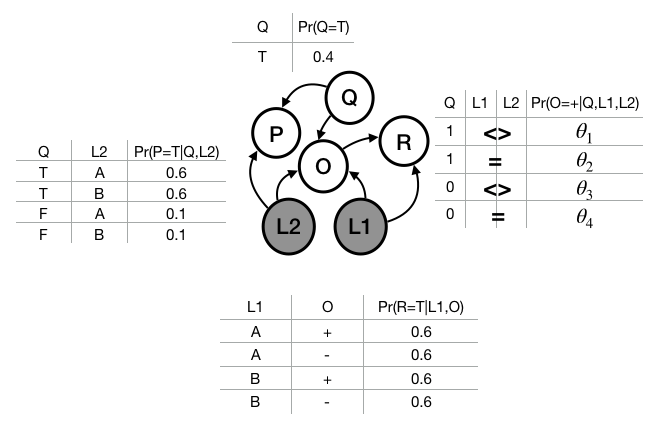
\includegraphics[width=\textwidth]{figs/BN.png}
  \end{minipage}\hfill
  \begin{minipage}[c]{0.45\textwidth}
    \caption{
        \small The model used for generating the datasets. There are four binary random variables, P, Q, O, and R. \textbf{P}: indicates whether or not the employee has high performance; \textbf{Q}: indicates whether or not an employee has high qualification; \textbf{O}: indicates whether or not the colleague submits the positive opinion towards the employee;  \textbf{R}: indicates whether or not the colleague has a positive opinion towards the employee;  \textbf{L1, L2}: indicates the label of the review provider and review receiver (observed).
    } \label{fig:BN}
  \end{minipage}
\end{figure}

We show the effectiveness of FairPSL by performing an empirical evaluation. We investigate two research questions in our experiments:
\begin{description}
\item[Q1] What is the effect of the fairness threshold $\delta$ on the fairness measures $RD/RC/RR$?
\item[Q2] How is decision quality affected by imposing $\delta$-fairness constraints?
\end{description}

Note that although we present the result for specific parameters of the framework in this section, we ran extensive analysis and the results we present are representative. We implemented the MAP inference routines of PSL and FairPSL in Python, using Gurobi-8.1\footnote{\url{www.gurobi.com}} as the backend solver. The FairPSL code, code for the data generator and data is publicly available\footnote{https://github.com/gfarnadi/FairPSL}. 

\subsection{Data generation}
  
We evaluate the FairPSL inference algorithm on synthetic datasets representing the performance review scenario (introduced in Example~\ref{ex:review}). The organization hierarchy is generated synthetically. 
The organization hierarchy generator is parameterized by two numbers: the number of employees in the organization ($n$) and the number of employees managed by each manager ($k$). Each employee is randomly assigned with a label \emph{A} or \emph{B}. An examples organization hierarchy with $n$=50 and $k$=3 is shown in Figure~\ref{fig:hierachy}.

\begin{figure}
  \begin{minipage}[c]{0.3\textwidth}
    \caption{
        \small An example of an organizational hierarchy with five levels and 50 employees with k=3. Each employee either has label A (shown with grey) or B (shown with white).
    }\label{fig:hierachy} 
	\end{minipage} \hfill
    \begin{minipage}[c]{0.7\textwidth}
    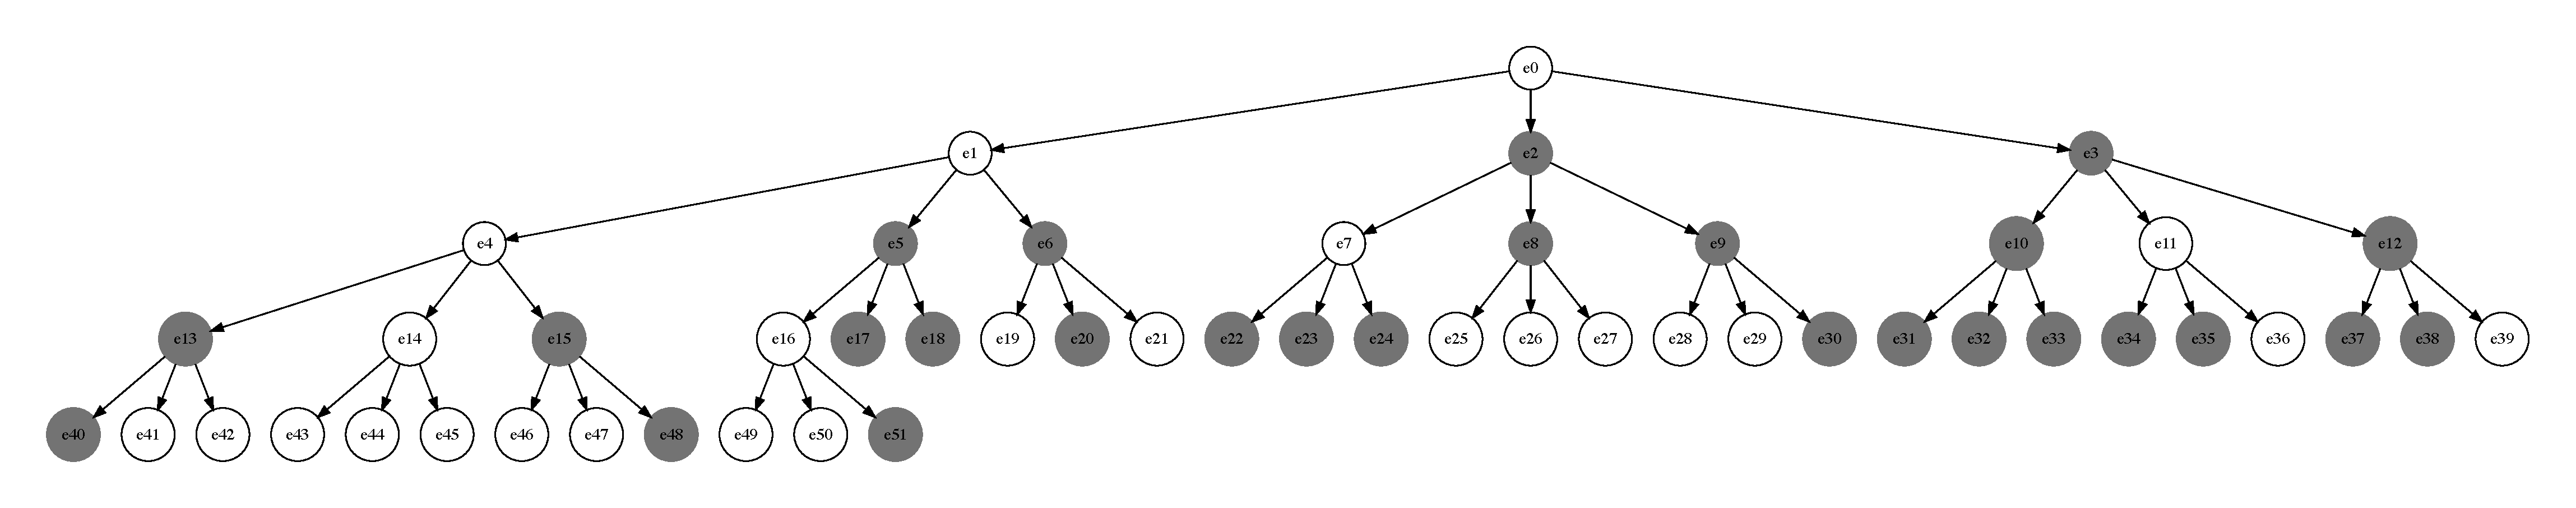
\includegraphics[width=\textwidth]{figs/Uni-hierachy.pdf}
  \end{minipage}
\end{figure}

For each employee, we use the generative model of Figure~\ref{fig:BN} to draw assignments for all the random variables. We assume that only $40\%$ of employees are qualified for promotion and regardless of their labels, employees submit only $60\%$ of their opinions. In addition, due to various personal and environmental factors, only $60\%$ of high quality employees perform well while $10\%$ of low quality employees also perform well regardless of their labels. Note that these numbers are not specific and just chosen for the framework to serve as a representative setting and a proof of concept. The conditional probability table for the opinion variable $O$ is parameterized by four values $(\theta_1, \theta_2, \theta_3, \theta_4)$ which together determine the degree of discrimination against the protected group. Since other parameters in the Bayesian network did not have a direct effect on the degree of discrimination, we fixed them to arbitrary values. 

The results presented in this section are based on an organization hierarchy  with $100$ employees where $k=5$. However, the results of the framework are not sensitive to the settings as we test the framework with various organization sizes ranging from $50$ to $500$ employees and various degree for $k$ ranging from $3$ to $10$. We generated seven datasets given the organization hierarchy using different values for the $\theta$ parameters: $(0.0,1.0,0.0,0.0)$, $(0.33,1.0,0.0,0.0)$, $(0.66,1.0,0.0,0.0)$, $(1.0,1.0,0.0,0.0)$, $(1.0,1.0,0.0,0.33)$, $(1.0,1.0,0.0,0.66)$, $(1.0,1.0,0.0,1.0)$. 
 
In the first three settings the discrimination originates from negative opinions towards qualified outgroup employees. The first setup is an extreme case where the opinion towards outgroup employees is always negative. The discrimination in the last three settings originates from positive opinions towards unqualified ingroup employees. The last setup is an extreme case where the opinion towards ingroup employees is always positive. The fourth setup represent unbiased opinions where employees are treated similarly based on their qualification. 

\paragraph{MAP Inference} We use the model presented in Table~\ref{tab:pslmodel} for MAP inference in PSL and FairPSL (recall that in FairPSL, the $\delta$-fairness constraints corresponding to one of the fairness measures are also added to the model). The observed atoms are $\textit{Manager(m,e)}$, $\textit{PositiveReview(e1,e2)}$ and labels of all employees. The truth values for all other atoms are obtained via MAP inference. We use the truth values obtained for the decision atoms $\textit{ToPromote(e)}$ to compute the fairness measures. We defined the discriminative pattern, and the protected and unprotected groups of this problem in Section~\ref{sec:formulation}.


\subsection{Evaluation results}

\begin{figure}
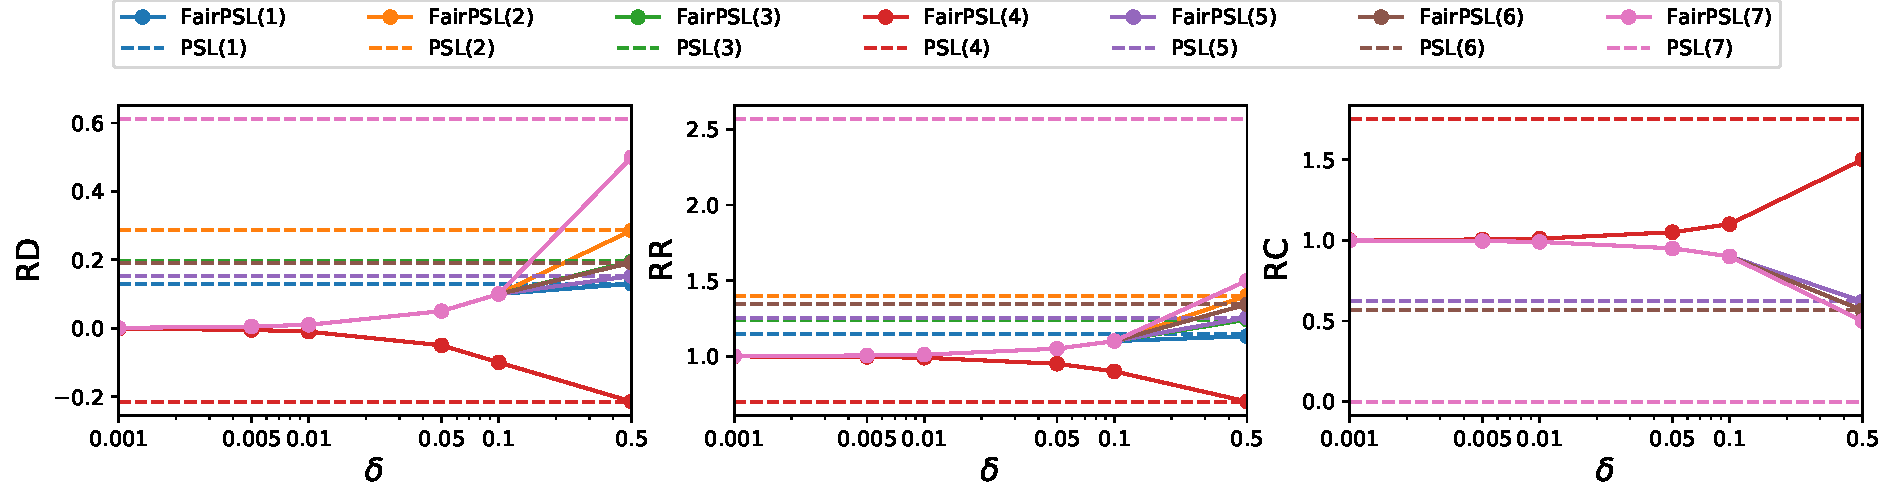
\includegraphics[width=1\linewidth]{figs/results_vis_uni_params.pdf}
\caption{\small Fairness score of predictions obtained by MAP inference of PSL and FairPSL, according to the fairness measures \emph{RD}, \emph{RR}, and \emph{RC}. The labels of datasets are mentioned with parenthesis next to the inference method. The FairPSL values of each measure are obtained by adding the $\delta$-fairness constraint of that measure.\label{fig:results}
}  
\end{figure}

To answer \textbf{Q1}, we run the MAP inference algorithm of PSL and FairPSL on seven synthetic datasets. 
We run the MAP inference of FairPSL multiple times on each dataset: For each of the three fairness measures, we add the corresponding $\delta$-fairness constraint with five thresholds $\{0.001, 0.005, 0.01, 0.05, 0.1, 0.5\}$.

Figure~\ref{fig:results} shows the fairness score of predictions in terms of the three fairness measures. As expected, tighter $\delta$-fairness constraints lead to better scores. Note that the best possible score according to RD is 0, as it computes a difference. Since RR and RC compute ratios, the best possible score according to these measures is 1. In our experiments, with any of these measures, taking $\delta = 0.001$ pushes the score of predictions to its limit.  

The $\delta$-fairness constraints modify the optimization problem of MAP inference by reducing the feasible region to solutions that conform with fairness guarantees. Research question \textbf{Q2} is concerned with the effect of this reduction on the accuracy of predictions. Note that decision quality is the same as the accuracy of predictions. To answer this question, we compare the inferred values for the decision atoms \textit{ToPromote(e)} against their actual values. These values are extracted from the known values of \textit{IsQualified(e)} according to rules 11 and 12 in Table~\ref{tab:pslmodel}. Figure~\ref{fig:accuracy} shows the area under the curve of the receiver operating characteristic~(AUC) of predicting the decision variable in three groups, namely the protected group, the unprotected group (i.e., promotion of the employees who have in-group managers), and all employees. By doing so, we make sure that our fairness constraints do not propagate bias towards either of the populations. Since the results of FairPSL with $\delta$-fairness constraints RR and RC are very similar to the results of RD, we only report the latter here.


\begin{figure}
    \centering
    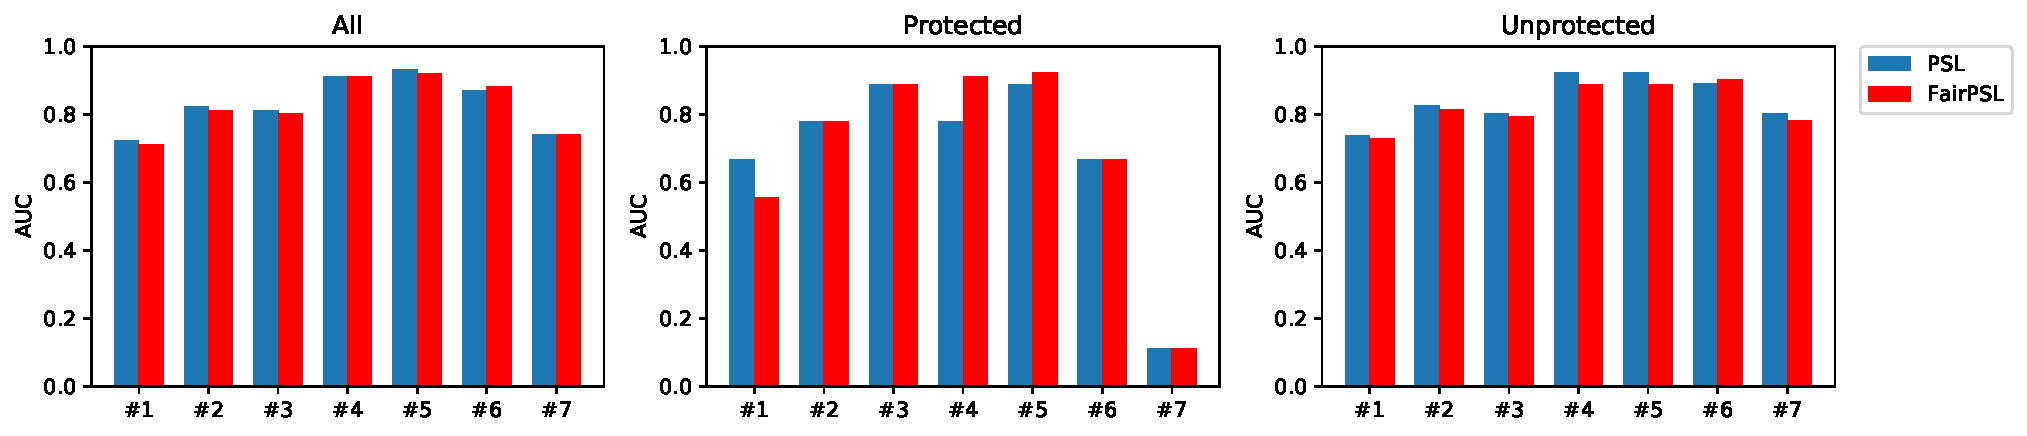
\includegraphics[width=\textwidth]{figs/roc.pdf}
    \caption{\small AUC score of predictions for truth values of unknown atoms \textit{ToPromote(e)} using MAP inference of PSL and FairPSL with $\delta$-fairness constraints $RD$ with $\delta=0.001$.}
    \label{fig:accuracy}
\end{figure}

According to Figure~\ref{fig:accuracy}, the results of both PSL and FairPSL in all seven datasets are close to each other. Note that although fairness may impose a cost in terms of overall accuracy, FairPSL often improves the accuracy of the protected class. Sometimes the overall predictions of FairPSL are even slightly better than PSL (e.g., dataset 6 and 7). As expected, the accuracy of the fourth setting where the opinions are unbiased are similar in both PSL and FairPSL. We observe that prediction of MAP inference for both FairPSL and PSL are similar, thus, in these settings at least, FairPSL guarantees fairness without hurting accuracy. Further investigation is required on the effect of the various ranges of discrimination (i.e., $\theta_1$, $\theta_2$, $\theta_3$, $\theta_4$) on the prediction results of FairPSL.



We also generate various types of organizations in which labels are not uniformly distributed, e.g., one population only occurs at the bottom levels of an organization. While we did not observe any differences in the behavior of our method with respect to accuracy and fairness measure, we found that the degree of discrimination is higher in such organizations. Further investigations on the structure of an organization on discrimination is an interesting direction for future research. 

\section{Conclusion and Future Directions}
\label{sec:conclusion}
Many applications of AI and machine learning affect peoples' lives in important ways. While there is a growing body of work on fairness in AI and ML, it assumes an individualistic notion of fairness.   In this paper, we have proposed a general framework for relational fairness which includes both a rich language for defining discrimination patterns and an efficient algorithm for performing inference subject to fairness constraints. We show our approach enforces fairness guarantees while preserving the accuracy of the predictions. 

There are many avenues for expanding on this work. For example, here we assumed that the discriminative pattern is given, however an automatic mechanism to extract discriminatory situations hidden in a large amount of decision records is an important and required task. Discrimination discovery has been studied for attribute-based fairness~\cite{pedreschi2013discovery}. An interesting next step is discrimination pattern discovery in relational data.

\section*{Acknowledgements}
This work is supported by the National Science Foundation under Grant Numbers CCF-1740850 and IIS-1703331. Golnoosh Farnadi and Behrouz Babaki are  supported by postdoctoral scholarships from IVADO through the Canada First Research Excellence Fund (CFREF) grant.

\begin{thebibliography}{10}
\itemsep=1pt 
\begin{small}

\bibitem{EUlaw}
European union legislation. (a) racial equality directive, 2000; (b) employment
  equality directive, 2000; (c) gender employment directive, 2006; (d) equal
  treatment directive (proposal), 2008.

\bibitem{UKlaw}
{UK} legislation. (a) sex discrimination act, 1975, (b) race relation act,
  1976.

\bibitem{USlaw}
United nations legislation. (a) universal declaration of human rights, 1948,
  (c) convention on the elimination of all forms of racial discrimination,
  1966, (d) convention on the elimination of all forms of discrimination
  against women, 1979.

\bibitem{alshukaili:iswc16}
Duhai Alshukaili, Alvaro A.~A. Fernandes, and Norman~W. Paton.
\newblock Structuring linked data search results using probabilistic soft
  logic.
\newblock In {\em International Semantic Web Conference {(1)}}, volume 9981 of
  {\em Lecture Notes in Computer Science}, pages 3--19, 2016.

\bibitem{bach:jmlr17}
Stephen~H. Bach, Matthias Broecheler, Bert Huang, and Lise Getoor.
\newblock Hinge-loss markov random fields and probabilistic soft logic.
\newblock {\em Journal of Machine Learning Research}, 18:109:1--109:67, 2017.

\bibitem{barocas2016big2}
Solon Barocas and Andrew~D Selbst.
\newblock Big data's disparate impact.
\newblock {\em California Law Review}, 104:671, 2016.

\bibitem{boyd2014networked}
Danah Boyd, Karen Levy, and Alice Marwick.
\newblock The networked nature of algorithmic discrimination.
\newblock In {\em Data and discrimination: Collected essays}, pages 53--57.
  2014.

\bibitem{brewer1979group}
Marilynn~B Brewer.
\newblock In-group bias in the minimal intergroup situation: A
  cognitive-motivational analysis.
\newblock {\em Psychological bulletin}, 86(2):307, 1979.

\bibitem{brewer2007social}
Marilynn~B Brewer.
\newblock The social psychology of intergroup relations: Social categorization,
  ingroup bias, and outgroup prejudice.
\newblock {\em Social Psychology: Handbook of Basic Principles}, 2007.

\bibitem{chouldechova2017fair2}
Alexandra Chouldechova.
\newblock Fair prediction with disparate impact: {A} study of bias in
  recidivism prediction instruments.
\newblock {\em CoRR}, abs/1703.00056, 2017.

\bibitem{dwork2012fairness3}
Cynthia Dwork, Moritz Hardt, Toniann Pitassi, Omer Reingold, and Richard~S.
  Zemel.
\newblock Fairness through awareness.
\newblock In {\em {ITCS}}, pages 214--226. {ACM}, 2012.

\bibitem{ebrahimi:emnlp16}
Javid Ebrahimi, Dejing Dou, and Daniel Lowd.
\newblock Weakly supervised tweet stance classification by relational
  bootstrapping.
\newblock In {\em {EMNLP}}, pages 1012--1017. The Association for Computational
  Linguistics, 2016.

\bibitem{farnadi2018fairness}
Golnoosh Farnadi, Behrouz Babaki, and Lise Getoor.
\newblock Fairness in relational domains.
\newblock In {\em AAAI/ACM Conference on AI, Ethics, and Society (AIES)}, pages
  108--114. ACM, 2018.

\bibitem{feldman2015certifying2}
Michael Feldman, Sorelle~A. Friedler, John Moeller, Carlos Scheidegger, and
  Suresh Venkatasubramanian.
\newblock Certifying and removing disparate impact.
\newblock In {\em {KDD}}, pages 259--268. {ACM}, 2015.

\bibitem{getoor2007introduction}
Lise Getoor and Ben Taskar.
\newblock {\em {Introduction to Statistical Relational Learning}}.
\newblock MIT press Cambridge, 2007.

\bibitem{hardt2016equality3}
Moritz Hardt, Eric Price, and Nati Srebro.
\newblock Equality of opportunity in supervised learning.
\newblock In {\em {NIPS}}, pages 3315--3323, 2016.

\bibitem{kamishima2011fairness}
Toshihiro Kamishima, Shotaro Akaho, and Jun Sakuma.
\newblock Fairness-aware learning through regularization approach.
\newblock In {\em ICDMW}, pages 643--650. {IEEE} Computer Society, 2011.

\bibitem{kouki:recsys15}
Pigi Kouki, Shobeir Fakhraei, James~R. Foulds, Magdalini Eirinaki, and Lise
  Getoor.
\newblock Hyper: {A} flexible and extensible probabilistic framework for hybrid
  recommender systems.
\newblock In {\em RecSys}, pages 99--106. {ACM}, 2015.

\bibitem{counterfactualfairness}
Matt~J. Kusner, Joshua~R. Loftus, Chris Russell, and Ricardo Silva.
\newblock Counterfactual fairness.
\newblock In {\em {NIPS}}, pages 4069--4079, 2017.

\bibitem{Pedreschi:2012}
Dino Pedreschi, Salvatore Ruggieri, and Franco Turini.
\newblock A study of top-k measures for discrimination discovery.
\newblock In {\em {SAC}}, pages 126--131. {ACM}, 2012.

\bibitem{pedreschi2013discovery}
Dino Pedreschi, Salvatore Ruggieri, and Franco Turini.
\newblock The discovery of discrimination.
\newblock In {\em Discrimination and Privacy in the Information Society},
  volume~3 of {\em Studies in Applied Philosophy, Epistemology and Rational
  Ethics}, pages 91--108. Springer, 2013.

\bibitem{ridgeway2004unpacking}
Cecilia~L Ridgeway and Shelley~J Correll.
\newblock Unpacking the gender system: A theoretical perspective on gender
  beliefs and social relations.
\newblock {\em Gender \& society}, 18(4):510--531, 2004.

\bibitem{sridhar:bioinformatics16}
Dhanya Sridhar, Shobeir Fakhraei, and Lise Getoor.
\newblock A probabilistic approach for collective similarity-based drug-drug
  interaction prediction.
\newblock {\em Bioinformatics}, 32(20):3175--3182, 2016.

\bibitem{verma2018fairness2}
Sahil Verma and Julia Rubin.
\newblock Fairness definitions explained.
\newblock In {\em 2018 IEEE/ACM International Workshop on Software Fairness
  (FairWare)}, pages 1--7. IEEE, 2018.

\bibitem{west2014exploiting}
Robert West, Hristo~S. Paskov, Jure Leskovec, and Christopher Potts.
\newblock Exploiting social network structure for person-to-person sentiment
  analysis.
\newblock {\em {TACL}}, 2:297--310, 2014.

\bibitem{zafar2017parity}
Muhammad~Bilal Zafar, Isabel Valera, Manuel Gomez{-}Rodriguez, Krishna~P.
  Gummadi, and Adrian Weller.
\newblock From parity to preference-based notions of fairness in
  classification.
\newblock In {\em {NIPS}}, pages 228--238, 2017.

\bibitem{zemel2013learning}
Richard~S. Zemel, Yu~Wu, Kevin Swersky, Toniann Pitassi, and Cynthia Dwork.
\newblock Learning fair representations.
\newblock In {\em {ICML} {(3)}}, volume~28 of {\em {JMLR} Workshop and
  Conference Proceedings}, pages 325--333. JMLR.org, 2013.

\end{small}
\end{thebibliography}

\end{document}

\end{article}


\begin{article}
{doppioDB 1.0: Machine Learning inside a Relational Engine}
{Gustavo Alonso, Zsolt Istvan, Kaan Kara, Muhsen Owaida, David Sidler}
\graphicspath{{submissions/gustavo/}}
%\documentclass[11pt,dvipdfm]{article}
\documentclass[11pt]{article}
\usepackage{deauthor,times,graphicx} %required
\usepackage{amsmath,amssymb}
\usepackage{multirow}
\usepackage{algorithm}
\usepackage{algpseudocode}
\usepackage{todonotes}
\usepackage{url}

% \graphicspath{{farnadi/}}

\newtheorem{mydef}{\textbf{Definition}}
\newtheorem{myex}{\textbf{Example}}
\newtheorem{mytheorem}{\textbf{Theorem}}


\begin{document}

\title{A Declarative Approach to Fairness in Relational Domains}
\author{Golnoosh Farnadi$^{1,2}$, Behrouz Babaki$^1$, Lise Getoor$^3$\\
$^1$Polytechnique Montr\'{e}al, $^2$ Mila, $^3$ UC Santa Cruz \\
farnadig@mila.quebec, behrouz.babaki@polymtl.ca, getoor@soe.ucsc.edu}

\maketitle

\begin{abstract}
AI and machine learning tools are being used with increasing frequency for decision making in domains that affect peoples' lives such as employment, education, policing and %loan approval
financial qualifications. These uses raise concerns about biases of algorithmic discrimination and have motivated the development of fairness-aware machine learning. However, existing fairness approaches are based solely on attributes of individuals. In many cases, discrimination is much more complex, and taking into account the social, organizational, and other connections between individuals is important. We introduce new notions of fairness that are able to capture the relational structure in a domain. We use first-order logic to provide a flexible and expressive language for specifying complex relational patterns of discrimination. Furthermore, we extend an existing statistical relational learning framework, probabilistic soft logic~(PSL), to incorporate our definition of relational fairness. We refer to this fairness-aware framework FairPSL. FairPSL makes use of the logical definitions of fairnesss but also supports a probabilistic interpretation. In particular, we show how to perform maximum a posteriori~(MAP) inference by exploiting probabilistic dependencies within the domain while avoiding violations of fairness guarantees. Preliminary empirical evaluation shows that we are able to make both accurate and fair decisions.
\end{abstract}

\section{Introduction}
\label{sec:introduction}

Over the past few years, AI and machine learning have become essential components in operations that drive the modern society, e.g., in financial, administrative, and educational spheres. \emph{Discrimination} happens when qualities of individuals which are not relevant to the decision making process influence the decision. Delegating decision making to an automated process raises questions about discriminating against individuals with certain traits based on biases in the data. This is especially important when the decisions have the potential to impact the lives of individuals, for example, the decisions on granting loans, assigning credit, and employment. 

\emph{Fairness} is defined as the absence of discrimination in a decision making process. The goal of \emph{fairness-aware} machine learning is to ensure that the decisions made by an algorithm do not discriminate against a population of individuals~\cite{feldman2015certifying2,boyd2014networked,hardt2016equality3}. Fairness has been well studied in the social sciences and legal scholarship (for an in-depth review see~\cite{barocas2016big2}), and there is emerging work on fairness-aware ML within the AI and computer science communities. For example, fairness through awareness/Lipschitz property~\cite{dwork2012fairness3}, individual fairness~\cite{zemel2013learning}, statistical parity/group fairness~\cite{kamishima2011fairness}, counterfactual fairness~\cite{counterfactualfairness}, demographic parity/disparate impact~\cite{feldman2015certifying2,chouldechova2017fair2}, preference-based fairness~\cite{zafar2017parity}, and equality of opportunity~\cite{hardt2016equality3}.

The existing work in fairness-aware machine learning is based on a definition of discrimination where a decision is influenced by an \emph{attribute} of an individual. An attribute value upon which discrimination is based (such as gender, race, or religion) is called a \emph{sensitive attribute}. The sensitive attribute defines a population of vulnerable individuals known as the \emph{protected group}. A fair decision-making process treats the protected group the same as the \emph{unprotected group}. 

However, in many social contexts, discrimination is the result of complex interactions and can not be described solely in terms of attributes of an individual. For example, consider an imaginary scenario in an organization in which younger female workers who have older male supervisors have lower chances of promotion than their male counterparts.\footnote{Of course, many other patterns may be possible: female bosses may promote female subordinates and discriminate against male workers, or male bosses may promote female employees.  Our goal is to provide a general framework which is able to describe arbitrarily complex discrimination patterns.} 
 This discrimination pattern involves two attributes of the individual (gender and age), a relationship with another individual (supervisor), and two attributes of the second individual. Addressing such complex cases poses two challenges. First, the concepts of discrimination and fairness need to be extended to capture not only attributes of individuals but also the relationships between them. Second, a process is required that ensures that fair decisions are made about individuals who are affected by such patterns. In this paper we address both of these challenges.
We use first-order logic (FOL) to extend the notion of fairness to the relational setting. FOL is an expressive representation for relational problems which is also widely used for learning in relational domains. Moreover, we extend an existing framework for statistical relational learning~\cite{getoor2007introduction} called probabilistic soft logic (PSL)\footnote{http://psl.linqs.org/}~\cite{bach:jmlr17}. PSL combines logic and probability for learning and reasoning over uncertain relational domains. One of the most common reasoning tasks in PSL is called maximum a posteriori (MAP) inference, which is performed by finding the most probable truth values for unknowns over a set of given evidence. We develop a new MAP inference algorithm which is able to maximize the a posteriori values of unknown variables \emph{subject to} fairness guarantees. An early version of this paper which this work builds upon and extends appeared in~\cite{farnadi2018fairness}.

\looseness-1
Our contributions are as follows: 1) we propose fairness-aware machine learning for the relational setting; 2) we extend PSL into a fairness-aware framework called FairPSL which can represent the logical definition of fairness; 3) we develop a new MAP inference algorithm which is able to maximize the posteriori values of unknown variables \emph{subject to} fairness guarantees; 4) we empirically evaluate our proposed framework on synthetic data. 

\section{Motivation}
\label{sec:motivation}

Discrimination in social contexts have been studied in the field of social psychology~\cite{brewer2007social,brewer1979group,ridgeway2004unpacking}. There is a large literature on various aspects of relational bias in social contexts such as \emph{in-group-out-group bias}, \emph{gender bias}, and \emph{ethnicity-based favoritism} that can result in discrimination. 
As an example, consider gender bias in the workplace that reflects stereotypically masculine criteria and male-based favoritism. Such gender bias 
typically places women in lower positions and negatively impacts their opportunities. Further, lack of women in leadership positions may affect the promotion of women and results in a glass ceiling that keeps women from rising beyond a certain level in the hierarchy. This scenario shows that considering  protected attributes such as gender is not always sufficient to detect the source of bias and avoid discrimination, one also has to consider the relational information, in this case the organization hierarchy. Note that this can be generalized to any ingroup/outgroup scenario where the sensitive attribute could be race, religion, age, marital-status, etc.

The existing work on designing fair algorithms in machine learning exclusively focuses on \emph{attribute-based fairness}, which is based on the following assumptions: First, there is an assumption that the individuals (sometimes referred to as units or entities) are independent and described by simple attribute vectors. Second, the group for which one wishes to ensure fairness (known as the \emph{protected group}) is defined on the basis of some attribute values. Finally, there is a decision that is associated with each individual, and the goal is to ensure that members of the protected group are subject to a fair decision (we discuss different fairness measures in Section~\ref{sec:fairnessmeasure}).  We illustrate  attribute-based fairness in the following example. 

\begin{myex}[Loan Processing]
\label{ex:loan}
A bank bases its decisions about granting a loan on attributes of the applicant. The goal is to decide whether to grant a loan to an applicant using a predictive model. The bank needs to ensure that the obey fair lending practices and ensure that gender, race, sexual orientation of applicants has no influence on the decision. In this scenario, the protected group is the historically disadvantaged applicants.  
\end{myex}
The current fairness-aware machine learning techniques are not capable of modeling relations and hence cannot be used to make the decision making model fair. However, in many decision making scenarios, especially in social and organizational settings, the domain is relational, and the protected group itself might be best represented using a relational definition. We illustrate this setting in the following scenario:
\begin{myex}[Performance Review]
\label{ex:review}
Consider an organization where decisions about the promotion of employees is based on two criteria: 1) an objective performance measure, and 2) the opinion of their direct and indirect managers above them. The opinions are inferred from the performance reviews which are collected periodically. Not every manager can submit a review for all its subordinates, this is especially the case for top-level managers who have a large number of subordinates. Hence, the opinions of managers are collectively inferred from the opinions of their sub-ordinates. However, some employees may be biased, and judge other employees unfavorably, by favoring employees who are similar to themselves (same gender, race, religion, etc.) over employees who are dissimilar. The organization needs to ensure that promotion of employees do not have any relational bias caused by in-group-out-group favoritism.

\end{myex}
Example~\ref{ex:review} describes a prediction problem over a database that consists of relations between employees. Such prediction tasks are best handled by techniques from the relational learning domain. To ensure fair prediction in such settings, we need to extend the notion of \emph{attribute-based fairness} to \emph{relational fairness}. Throughout this paper, we use the performance review problem as a running example for relational fairness.

\section{Fairness Formalism}
\label{sec:formulation}

A representation that can describe different types of entities and different relationships between them is called relational. In this section, we use first-order logic to define relational fairness. We employ first-order logic as an expressive representation formalism which can represent objects and complex relationships between them. We start by defining an atom:

\begin{mydef}[Atom]
An atom is an expression of the form $P(a_1, a_2, \ldots, a_n)$ where each argument $a_1, a_2,$ $\ldots,$ $a_n$ is either a constant or a variable. The finite set of all possible substitutions of a variable to a constant for a particular variable $a$ is called its \textit{domain} $D_{a}$. If all variables in $P(a_1, a_2, \ldots, a_n)$ are substituted by some constant from their respective domain, then we call the resulting atom a \textit{ground atom}. 
\end{mydef}

\begin{myex}
In our loan processing problem (Example~\ref{ex:loan}), we can represent applicants' attributes by atoms. For instance, atom $Female(v)$ indicates whether or not applicant $v$ is female. Similarly, we can represent relations with atoms. In the performance review problem in Example~\ref{ex:review} the atom $Manager(m,e)$ indicates whether or not employee $m$ is a direct or indirect manager of employee $e$.
\end{myex}

The relational setting provides the flexibility to express complex definitions with formulae.

\begin{mydef}[Formula] 
A formula is defined by induction: every atom is a formula. If $\alpha$ and $\beta$ are formulae, then $\alpha \vee \beta$, $\alpha \wedge \beta$, $\neg \alpha$, $\alpha \rightarrow \beta$ are formulae. If $x$ is a variable and $\alpha$ is a formula, then the quantified expressions of the form $\exists x$ $\alpha$ and $\forall x$ $\alpha$ are formulae.    
\end{mydef}

To characterize groups of individuals based on a formula, we define the notion of \emph{population}.

\begin{mydef}[Population]
We denote formula $F$ which has only one free variable $v$ (i.e., other variables in $F$ are quantified) by $F[v]$. The population defined by $F[v]$ is the set of substitutions of $v$ for which $F[v]$ holds.   
\end{mydef}


\begin{myex}
\label{ex:disformula}
Consider the formula $F[v] := \forall u, \, \textit{Manager}(u,v) \rightarrow \neg \textit{SameGroup}(u, v)$. The population specified by this formula is the set of individuals all of whose managers belong to a group different from theirs. 
\end{myex}

The truth value of a formula is derived from the truth value of atoms that it comprises, according to the rules of logic. Each possible assignment of truth values to ground atoms is called an \emph{interpretation}. 


\begin{mydef}[Interpretation]
An interpretation $I$ is a mapping that associates a truth value $I(P)$ to each ground atom $P$. For Boolean truth values, $I$ associates true to 1 and false to 0 truth values. For soft logic (see Definition~\ref{def:softlogic}) $I$ maps each ground atom $P$ to a truth value in interval $[0, 1]$.
\end{mydef}

In attribute-based fairness, it is assumed that there is a certain attribute of individuals, i.e, the sensitive attribute,  that we do not want to affect a decision. Gender, race, religion and marital status are examples of sensitive attributes. Discrimination has been defined in social science studies as a treatment in favor or against a group of individuals given their sensitive attribute. This group of individuals is the protected group. 

In a relational setting, both the sensitive attributes of an individual and their participation in various relations may have an undesired effect on the final decision. We characterize the protected group in a relational setting by means of a population. In practice, we are often interested in maintaining fairness for a specific population such as applicants, students, employees, etc. This population is then partitioned into the protected and unprotected groups. We define a \emph{discriminative pattern} which is a pair of formulae to capture these groups: 1) $F_1[v]$: to specify the difference between the protected and unprotected groups and 2) $F_2[v]$: to specify the population over which we want to maintain fairness. 

\begin{mydef}[Discriminative pattern]
A discriminative pattern is a pair $\textit{DP}[v]:=(F_1[v], F_2[v])$ , where $F_1[v]$ and $F_2[v]$ are formulae.
\end{mydef}

\begin{myex}
\label{ex:pattern}
The two formulae in the discrimination pattern $\textit{DP}[v]:= \big((\forall u, \,  \textit{Manager}(u,v) \rightarrow  \neg \textit{SameGroup}(u, v)),$ $\textit{Employee}(v)\big)$ specify two populations, namely all employees and those employees who belong to a group different from their managers.
\end{myex}

Given the definition of the discriminative pattern, we have a rich language to define the scope of the protected and unprotected groups in a relational setting.

\begin{mydef}[Protected group] Given an interpretation $I$, the protected group is a population of the form:
{$$PG :=\{ v : F_1[v] \wedge F_2[v]\}$$}
which is defined as the set of all instances hold for variable $v$ for which $F_1[v] \wedge F_2[v]$ is true under interpretation $I$, that is, $I(F_1[v] \wedge F_2[v]) = 1$. 
Similarly, the \emph{unprotected group} is a population of the form: 
{$$UG := \{ v : \neg F_1[v] \wedge  F_2[v]\}$$}
which is defined as the set of all instances hold for variable $v$ 
for which $I(\neg F_1[v] \wedge F_2[v]) = 1$. 
\end{mydef}

\begin{myex}
The protected group of the discrimination pattern specified in Example~\ref{ex:pattern} is {$PG := \big\{ v : \big(\forall u, \,$ $ \textit{Manager}(u, v) \rightarrow \neg \textit{SameGroup}(u, v)\big) \wedge \textit{Employee}(v) \big\}$} and the unprotected group is {$UG :=  \big\{ v:  \big(\exists u, \, \textit{Manager}(u,v) \wedge \textit{SameGroup}(u, v)\big) \wedge \textit{Employee}(v) \big\}$}. This means our protected group is the set of employees belonging to a group different from their managers,
and our unprotected group consists of other employees. 
\end{myex}

Discrimination is defined in terms of a treatment or decision that distinguishes between the protected and unprotected groups. Here we define the \emph{decision} atom.
\begin{mydef}[Decision atom] A decision atom $d(v)$ is an atom containing exactly one variable $v$ that specifies a decision affecting the protected group which is defined either by law or end-user.
\end{mydef}
\begin{myex}
The decision atom ${\textit ToPromote}(v)$ indicates whether or not $v$ receives a promotion.
\end{myex}

Note that the fairness formulation in this section is designed for the relational setting, however relational fairness subsumes the attribute-based fairness such that: a sensitive attribute is defined by an atom with one argument and $F_2[v]$ in discrimination pattern is $\textit{Applicant}(v)$. For example, discrimination pattern of our loan processing problem in Example~\ref{ex:loan} is of the form $\textit{DP} := ( \textit{Female}(v), \textit{Applicant}(v))$ that denotes female applicants as the protected group (i.e., $PG :=  \{ v: \textit{Female}(v) \}$) and male applicants as the unprotected group (i.e., $UG := \{ v: \neg \textit{Female}(v)\}$).


\section{Fairness Measures}
\label{sec:fairnessmeasure}

Over the past few years, many fairness measures have been introduced~\cite{verma2018fairness2}. An important class of these measures are \emph{group fairness} measures which quantify the inequality between different subgroups. Some of the most popular measures in this class include \emph{equal opportunity}, \emph{equalized odds}, and \emph{demographic parity}~\cite{hardt2016equality3}. In this paper we restrict our focus to the latter. In an attribute-value setting, demographic parity means that the decision should be independent of the protected attributes. Assume that binary variables $A$ and $C$ denote the decision and protected attributes, and the preferred value of $A$ is one. Demographic parity requires that:

\begin{equation*}
    P(A=1 | C=0) = P(A=1 | C=1)
\end{equation*}

We will now generalize this measure to the relational setting using the notations defined in Section~\ref{sec:formulation}. Let $a$ and $c$ denote the counts of denial (i.e., negative decisions) for protected and unprotected groups, and $n_{1}$ and $n_{2}$ denote their sizes, respectively. Given the decision atom $d(v)$, discriminative pattern $\textit{DP}(F_1[v], F_2[v])$, and interpretation $I$, these counts are computed by the following equations: 
{
\begin{flalign}
    & a \equiv \sum_{v \in D_v} I\big( \neg d(v) \wedge  F_1[v] \wedge F_2[v]) \label{eq:a}\\
    & c \equiv \sum_{v \in D_v} I\big( \neg d(v) \wedge  \neg F_1[v] \wedge  F_2[v]) \label{eq:c}\\
    & n_{1} \equiv \sum_{v \in D_v} I\big(F_1[v] \wedge F_2[v]) \label{eq:n1}\\
    & n_{2} \equiv \sum_{v \in D_v} I\big(\neg F_1[v] \wedge  F_2[v]) \label{eq:n2}
\end{flalign}}
The proportions of denying for protected and unprotected groups are $p_1 = \frac{a}{n_1}$ and $p_2 = \frac{c}{n_2}$, respectively. There are a number of data-driven measures~\cite{Pedreschi:2012} which quantify demographic disparity and can be defined in terms of $p_1$ and $p_2$:
\begin{itemize}
    \item \textbf{Risk difference}: $RD = p_1 - p_2$, also known as absolute risk reduction. 
    \item \textbf{Risk Ratio}: $RR = \frac{p_1}{p_2}$, also known as relative risk. 
    \item \textbf{Relative Chance}: $RC = \frac{1 - p_1}{1 - p_2}$ also, known as selection rate.
\end{itemize}
These measures have been used in the legal systems of European Union, UK, and US~\cite{EUlaw,UKlaw,USlaw}. Notice that RR is the ratio of the proportion of benefit denial between the protected and unprotected groups, while RC is the ratio of the proportion of benefit granted. Finally, we introduce the notion of $\delta$-fairness.

\begin{mydef}[$\delta$-fairness]
If a fairness measure for a decision making process falls within some $\delta$-window, then the process is \emph{$\delta\text{-fair}$}. Given $0 \leq \delta \leq 1$, the  $\delta$-windows for measures RD/RR/RC are defined as:
{\begin{flalign*}
	     - \delta \leq &RD \leq \delta \\
	     1- \delta \leq &RR \leq 1+ \delta\\
	     1- \delta \leq &RC \leq 1+ \delta
	\end{flalign*}}
\end{mydef}

To overcome the limitations of attribute-based fairness, we introduce a new statistical relational learning~(SRL) framework~\cite{getoor2007introduction} suitable for modelling fairness in relational domain. In the next section, we review probabilistic soft logic~(PSL). We then extend PSL with the definition of relational fairness introduced above in Section~\ref{sec:fairMAP}. Our fairness-aware framework, ``FairPSL'', is the first SRL framework that performs fair inference. 

\section{Background: Probabilistic Soft Logic}
\label{sec:psl}

In this section, we review the syntax and semantics of PSL, and in the next section we extend MAP inference in PSL with fairness constraints to define MAP inference in FairPSL.

PSL is a probabilistic programming language for defining hinge-loss Markov random fields~\cite{bach:jmlr17}. Unlike other SRL frameworks whose atoms are Boolean, atoms in PSL can take continuous values in the interval $[0,1]$. PSL is an expressive modeling language that can incorporate domain knowledge with first-order logical rules and has been used successfully in various domains, including bioinformatics~\cite{sridhar:bioinformatics16}, recommender systems~\cite{kouki:recsys15}, natural language processing~\cite{ebrahimi:emnlp16}, information retrieval~\cite{alshukaili:iswc16}, and social network analysis~\cite{west2014exploiting}, among many others. 
 
A PSL model is defined by a set of first-order logical rules called \emph{PSL rules}.

\begin{mydef} [PSL rule] a PSL rule $r$ is an expression of the form:
{\begin{equation}
\lambda_{r}: T_1 \land T_2 \land \ldots \land T_w \rightarrow H_1 \vee H_2 \vee \ldots \vee H_l
\end{equation}}

where { $T_1, T_2, \ldots, T_w, H_1, H_2, \ldots, H_l$} are atoms or negated atoms and { $\lambda_{r} \in \mathbb{R}^{+} \cup \infty$} is the weight of the rule $r$.  We call { $T_1 \land T_2 \land \ldots \land T_w$} the body of $r$ ($r_{body}$), and { $H_1 \vee H_2 \vee \ldots \vee H_l$} the head of $r$ ($r_{head}$).
\end{mydef}


Since atoms in PSL take on continuous values in the unit interval $[0,1]$, next we define soft logic to calculate the value of the PSL rules under an interpretation $I$.

\begin{mydef}[Soft logic]
\label{def:softlogic}
The ({$\tilde{\wedge}$}) and ({$\tilde{\vee}$}) and negation ({$\tilde{\neg}$}) are defined as follows. For {$m, n \in [0,1]$} we have: {$m \tilde{\wedge} n = \max(m+n -1, 0)$}, {$m \tilde{\vee} n = \min(m+n , 1)$} and {$\tilde{\neg} m = 1 - m$}. The $\, \tilde{} \,$ indicates the relaxation over Boolean values.
\end{mydef}

The probability of truth value assignments in PSL is determined by the rules' \emph{distance to satisfaction}.

\begin{mydef}[The distance to satisfaction]
The distance to satisfaction $d_{r}(I)$ of a rule $r$ under an interpretation $I$ is defined as:
{
\begin{equation}
d_{r}(I) = \max\{0, I(r_{body})-I(r_{head})\}
\end{equation}}
\end{mydef}

By using Definition~\ref{def:softlogic}, one can show that the closer the interpretation of a grounded rule $r$ is to 1, the smaller its distance to satisfaction. A PSL model induces a distribution over interpretations $I$. Let $R$ be the set of all grounded rules, then the probability density function is:
{
\begin{equation}
f(I) ={\frac{1}{Z}} \exp[-\sum_{r\in R} \lambda_{r}(d_{r}(I))^p]
\label{eq:potential}
\end{equation}
}
\noindent where { $\lambda_{r}$} is the weight of rule $r$, {
$Z = \int_{I} \exp[ -\sum_{r\in R} \lambda_{r}(d_{r}(I))^p]$
} is a normalization constant, and { $p \in \{1,2\}$} provides a choice of two different loss functions, $p=1$ (i.e., linear), and $p=2$ (i.e, quadratic). These probabilistic models are instances of hinge-loss Markov random fields~(HL-MRF)~\cite{bach:jmlr17}. The goal of maximum a posteriori (MAP) inference is to find the most probable truth assignments $I_{\textit{MPE}}$ of unknown ground atoms given the evidence which is defined by the interpretation $I$. Let $X$ be all the evidence, i.e., $X$ is the set of ground atoms such that $\forall x \in X, I(x)$ is known, and let $Y$ be the set of ground atoms such that $\forall y \in Y, I(y)$ is unknown. Then we have
{
\begin{equation}
I_{\textit{MAP}}(Y) = \textit{arg}\max_{I(Y)} P(I(Y)|I(X))
\end{equation}}
Maximizing the density function in Equation~\ref{eq:potential} is equivalent to minimizing the weighted sum of the distances to satisfaction of all rules in PSL. 

\begin{table*}[t]
    \centering
    \begin{tabular}{|lll|}
    \hline
    &&\\
    $R1$ & $\lambda_1$ &: $\textit{IsQualified}(e) \rightarrow \textit{HighPerformance}(e)$ \\
    $R2$ & $\lambda_1$ &: $\neg \textit{IsQualified}(e) \rightarrow \neg \textit{HighPerformance}(e)$ \\
    $R3$ & $\infty$ &: $\textit{PositiveReview}(e1, e2) \rightarrow \textit{PositiveOpinion}(e1, e2)$ \\
    $R4$ & $\infty$ &: $\neg \textit{PositiveReview}(e1, e2) \rightarrow \neg \textit{PositiveOpinion}(e1, e2)$ \\
    $R5$ & $\lambda_1$ &: $\textit{PositiveOpinion}(e1, e2) \wedge \textit{Manager}(m, e1) \rightarrow \textit{PositiveOpinion}(m, e2)$ \\
    $R6$ & $\lambda_1$ &: $\neg \textit{PositiveOpinion}(e1, e2) \wedge \textit{Manager}(m, e1) \rightarrow \neg \textit{PositiveOpinion}(m, e2)$ \\
    $R7$ & $\lambda_1$ &: $\textit{PositiveOpinion}(m, e) \wedge \textit{Manager}(m, e) \rightarrow \textit{IsQualified}(e)$ \\
    $R8$ & $\lambda_1$ &: $\neg \textit{PositiveOpinion}(m, e) \wedge \textit{Manager}(m, e) \rightarrow \neg \textit{IsQualified}(e)$ \\
    $R9$ &  $\lambda_1$ &: $\neg \textit{ToPromote}(e)$\\
    $R10$ & $\infty$ &: $\textit{IsQualified}(e) \rightarrow \textit{ToPromote}(e)$ \\
    $R11$ & $\infty$ &: $\neg \textit{IsQualified}(e) \rightarrow \neg \textit{ToPromote}(e)$ \\
    &&\\
    \hline
    \end{tabular}
    \caption{\small A simplified PSL model for the \emph{Performance Reviewing} problem}
    \label{tab:pslmodel}
\end{table*}

\begin{myex}
\label{ex:pslmodel}
The simplified PSL model for the performance reviewing problem in Example\ref{ex:review} is given in Table~\ref{tab:pslmodel}. The goal of MAP inference for this problem is to infer employees to promote. We simplified the model by assigning the same weight to all soft rules (i.e., $\lambda_i= 1$ where $i=\{1,2,5,6,7,8,9\}$). Below we explain the meaning of each rule in the model.

Rule $R1$ indicates that qualified employees have high performance and similarly rule $R2$ expresses that a negative qualification of employees is derived from their low performance. Rules $R5$ and $R6$ presents the propagation of opinion from bottom to top of the organizational hierarchy, i.e., managers have similar opinions towards employees given the opinions of their sub-ordinate managers. And rules $R7$ and $R8$ indicate that the positive/negative opinion of direct/indirect managers derive from the qualification of an employee. Rule $R9$ indicates the prior that not all employees get promoted. We also have four hard constraints (i.e., rules $R3$, $R4$, $R10$ and $R11$) where the weight of the rules are $\infty$. Rules $R3$ and $R4$ indicate that submitted positive/negative reviews should reflect positive/negative opinions. And two rules $R10$ and $R11$ show that a highly qualified employee should get promoted. 
\end{myex}

\section{Fairness-aware PSL (FairPSL)}
\label{sec:fairMAP}

The standard MAP inference in PSL aims at finding values that maximize the conditional probability of unknowns. Once a decision is made according to these values, one can use the fairness measure to quantify the degree of discrimination. A simple way to incorporate fairness in MAP inference is to add the $\delta$-fairness constraints to the corresponding optimization problem.   

Consider risk difference, $\textit{RD}$, where $\textit{RD} \equiv \frac{\mathbf{a}}{n_1} - \frac{\mathbf{c}}{n_2}$. The $\delta$-fairness constraint $-\delta \leq \textit{RD} \leq \delta$ can be encoded as the following constraints:
{\begin{align}
    & n_2 \mathbf{a} - n_1 \mathbf{c} - n_1 n_2 \delta \leq 0 \label{eq:RD1}\\
    & n_2 \mathbf{a} - n_1 \mathbf{c} + n_1 n_2 \delta \geq 0
\end{align}}
Similarly, from $\textit{RR} \equiv \frac{\mathbf{a} / n_1}{\mathbf{c} / n_2}$ and the $\delta$-fairness constraint $1 - \delta \leq \textit{RR} \leq 1 + \delta$ we obtain:
{\begin{align}
    & n_2 \mathbf{a} - (1 + \delta) n_1 \mathbf{c} \leq 0 \\
    & n_2 \mathbf{a} - (1 - \delta) n_1 \mathbf{c} \geq 0
\end{align}}
And finally, $\textit{RC} \equiv \frac{1 - \mathbf{a} / n_1}{1 - \mathbf{c} / n_2}$ and the $\delta$-fairness constraint $1 - \delta \leq \textit{RC} \leq 1 + \delta$ gives:
{ \begin{align}
    & - n_2 \mathbf{a} + (1 + \delta) n_1 \mathbf{c} - \delta n_1 n_2 \leq 0 \\
    & - n_2 \mathbf{a} + (1 - \delta) n_1 \mathbf{c} + \delta n_1 n_2 \geq 0 \label{eq:RC2}
\end{align}}
A primary advantage of PSL over similar frameworks is that its MAP inference task reduces to a convex optimization problem which can be solved in polynomial time. To preserve this advantage, we need to ensure that the problem will remain convex after the addition of $\delta$-fairness constraints. 

\begin{mytheorem}
The following condition is sufficient for preserving the convexity of MAP inference problem after addition of $\delta$-fairness constraints: The formulae $F_1[v]$ and $F_2[v]$ do not contain an atom $y \in Y$ and all atoms in $F_1[v]$ and $F_2[v]$ have values zero or one.
\end{mytheorem}
\begin{proof}
Since $I(F_1[v])$ and $I(F_2[v])$ do not depend on $I(Y)$, the values $n_{1}$ and $n_{2}$ are constants that can be computed in advance. Let us define the sets $D_v^a = \{ v \in D_v : F_1[v] \wedge F_2[v] \, \text{is true} \}$ and $D_v^c = \{ v \in D_v : \neg F_1[v] \wedge F_2[v] \, \text{is true} \}$. Since $F_1[v]$ and $F_2[v]$ can be only zero or one, we can rewrite the equations~\ref{eq:a} and \ref{eq:c} as:
{
\begin{align*}
    & \mathbf{a} = \sum_{v \in D_v^a} I(\neg d(v)) = |D_v^a| - \sum_{v \in D_v^a} I(d(v))\\
    & \mathbf{c} = \sum_{v \in D_v^c} I(\neg d(v)) = |D_v^c| - \sum_{v \in D_v^c} I(d(v))
\end{align*}}
\noindent which indicates that $\mathbf{a}$ and $\mathbf{c}$ can be expressed as linear combinations of variables in the optimization problem. This means that constraints~\ref{eq:RD1}-\ref{eq:RC2} are linear. Hence, addition of these constraints preserves the convexity of the optimization problem. 
\end{proof}

\section{Experiments}
\label{sec:experiment}

\begin{figure}
  \begin{minipage}[c]{0.6\textwidth}
    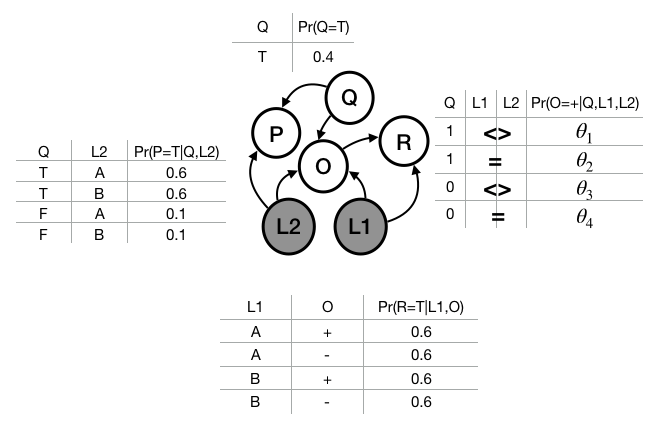
\includegraphics[width=\textwidth]{figs/BN.png}
  \end{minipage}\hfill
  \begin{minipage}[c]{0.45\textwidth}
    \caption{
        \small The model used for generating the datasets. There are four binary random variables, P, Q, O, and R. \textbf{P}: indicates whether or not the employee has high performance; \textbf{Q}: indicates whether or not an employee has high qualification; \textbf{O}: indicates whether or not the colleague submits the positive opinion towards the employee;  \textbf{R}: indicates whether or not the colleague has a positive opinion towards the employee;  \textbf{L1, L2}: indicates the label of the review provider and review receiver (observed).
    } \label{fig:BN}
  \end{minipage}
\end{figure}

We show the effectiveness of FairPSL by performing an empirical evaluation. We investigate two research questions in our experiments:
\begin{description}
\item[Q1] What is the effect of the fairness threshold $\delta$ on the fairness measures $RD/RC/RR$?
\item[Q2] How is decision quality affected by imposing $\delta$-fairness constraints?
\end{description}

Note that although we present the result for specific parameters of the framework in this section, we ran extensive analysis and the results we present are representative. We implemented the MAP inference routines of PSL and FairPSL in Python, using Gurobi-8.1\footnote{\url{www.gurobi.com}} as the backend solver. The FairPSL code, code for the data generator and data is publicly available\footnote{https://github.com/gfarnadi/FairPSL}. 

\subsection{Data generation}
  
We evaluate the FairPSL inference algorithm on synthetic datasets representing the performance review scenario (introduced in Example~\ref{ex:review}). The organization hierarchy is generated synthetically. 
The organization hierarchy generator is parameterized by two numbers: the number of employees in the organization ($n$) and the number of employees managed by each manager ($k$). Each employee is randomly assigned with a label \emph{A} or \emph{B}. An examples organization hierarchy with $n$=50 and $k$=3 is shown in Figure~\ref{fig:hierachy}.

\begin{figure}
  \begin{minipage}[c]{0.3\textwidth}
    \caption{
        \small An example of an organizational hierarchy with five levels and 50 employees with k=3. Each employee either has label A (shown with grey) or B (shown with white).
    }\label{fig:hierachy} 
	\end{minipage} \hfill
    \begin{minipage}[c]{0.7\textwidth}
    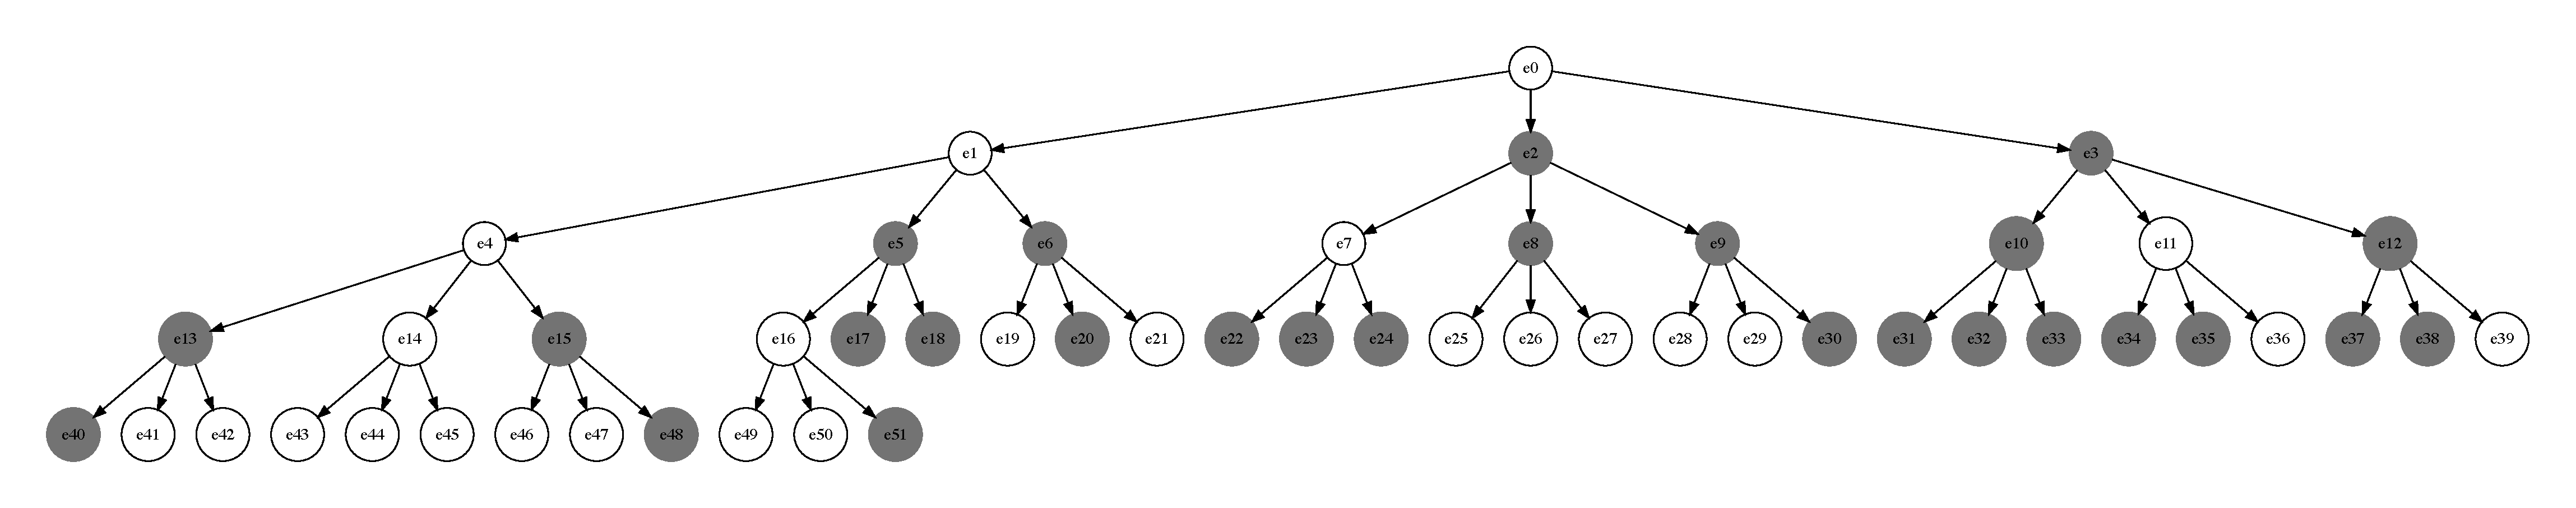
\includegraphics[width=\textwidth]{figs/Uni-hierachy.pdf}
  \end{minipage}
\end{figure}

For each employee, we use the generative model of Figure~\ref{fig:BN} to draw assignments for all the random variables. We assume that only $40\%$ of employees are qualified for promotion and regardless of their labels, employees submit only $60\%$ of their opinions. In addition, due to various personal and environmental factors, only $60\%$ of high quality employees perform well while $10\%$ of low quality employees also perform well regardless of their labels. Note that these numbers are not specific and just chosen for the framework to serve as a representative setting and a proof of concept. The conditional probability table for the opinion variable $O$ is parameterized by four values $(\theta_1, \theta_2, \theta_3, \theta_4)$ which together determine the degree of discrimination against the protected group. Since other parameters in the Bayesian network did not have a direct effect on the degree of discrimination, we fixed them to arbitrary values. 

The results presented in this section are based on an organization hierarchy  with $100$ employees where $k=5$. However, the results of the framework are not sensitive to the settings as we test the framework with various organization sizes ranging from $50$ to $500$ employees and various degree for $k$ ranging from $3$ to $10$. We generated seven datasets given the organization hierarchy using different values for the $\theta$ parameters: $(0.0,1.0,0.0,0.0)$, $(0.33,1.0,0.0,0.0)$, $(0.66,1.0,0.0,0.0)$, $(1.0,1.0,0.0,0.0)$, $(1.0,1.0,0.0,0.33)$, $(1.0,1.0,0.0,0.66)$, $(1.0,1.0,0.0,1.0)$. 
 
In the first three settings the discrimination originates from negative opinions towards qualified outgroup employees. The first setup is an extreme case where the opinion towards outgroup employees is always negative. The discrimination in the last three settings originates from positive opinions towards unqualified ingroup employees. The last setup is an extreme case where the opinion towards ingroup employees is always positive. The fourth setup represent unbiased opinions where employees are treated similarly based on their qualification. 

\paragraph{MAP Inference} We use the model presented in Table~\ref{tab:pslmodel} for MAP inference in PSL and FairPSL (recall that in FairPSL, the $\delta$-fairness constraints corresponding to one of the fairness measures are also added to the model). The observed atoms are $\textit{Manager(m,e)}$, $\textit{PositiveReview(e1,e2)}$ and labels of all employees. The truth values for all other atoms are obtained via MAP inference. We use the truth values obtained for the decision atoms $\textit{ToPromote(e)}$ to compute the fairness measures. We defined the discriminative pattern, and the protected and unprotected groups of this problem in Section~\ref{sec:formulation}.


\subsection{Evaluation results}

\begin{figure}
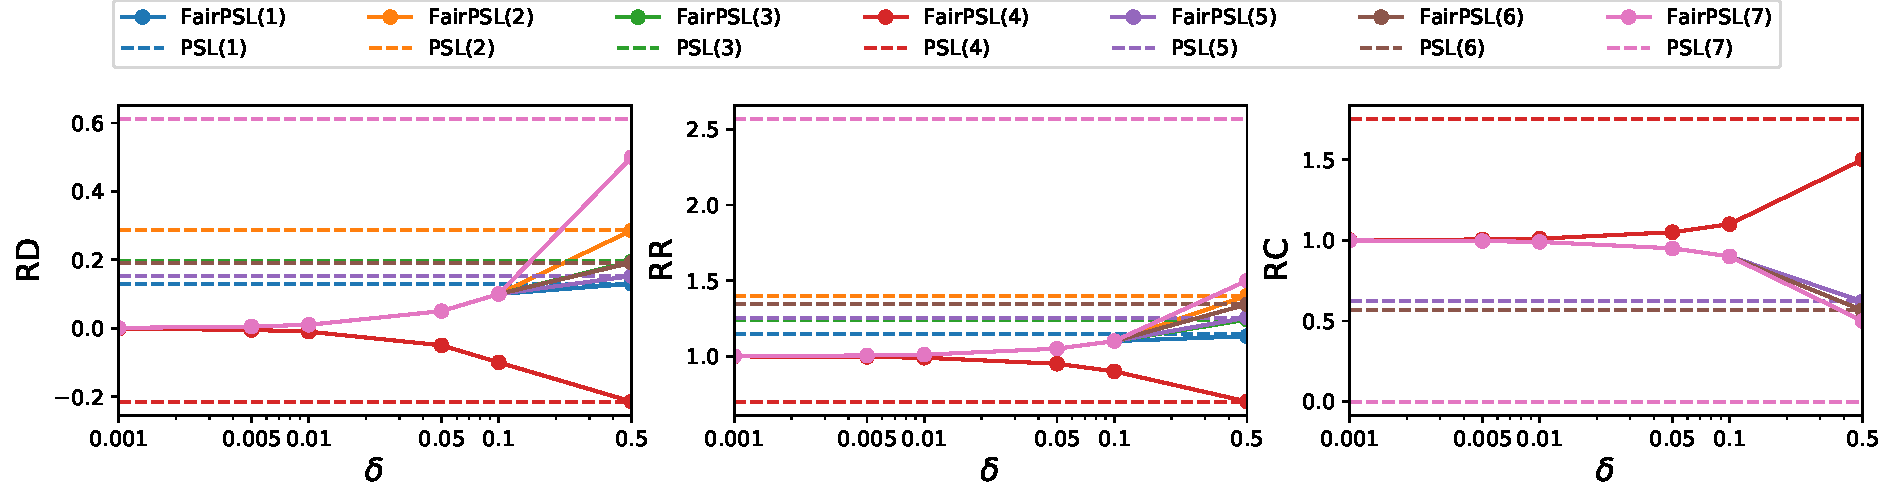
\includegraphics[width=1\linewidth]{figs/results_vis_uni_params.pdf}
\caption{\small Fairness score of predictions obtained by MAP inference of PSL and FairPSL, according to the fairness measures \emph{RD}, \emph{RR}, and \emph{RC}. The labels of datasets are mentioned with parenthesis next to the inference method. The FairPSL values of each measure are obtained by adding the $\delta$-fairness constraint of that measure.\label{fig:results}
}  
\end{figure}

To answer \textbf{Q1}, we run the MAP inference algorithm of PSL and FairPSL on seven synthetic datasets. 
We run the MAP inference of FairPSL multiple times on each dataset: For each of the three fairness measures, we add the corresponding $\delta$-fairness constraint with five thresholds $\{0.001, 0.005, 0.01, 0.05, 0.1, 0.5\}$.

Figure~\ref{fig:results} shows the fairness score of predictions in terms of the three fairness measures. As expected, tighter $\delta$-fairness constraints lead to better scores. Note that the best possible score according to RD is 0, as it computes a difference. Since RR and RC compute ratios, the best possible score according to these measures is 1. In our experiments, with any of these measures, taking $\delta = 0.001$ pushes the score of predictions to its limit.  

The $\delta$-fairness constraints modify the optimization problem of MAP inference by reducing the feasible region to solutions that conform with fairness guarantees. Research question \textbf{Q2} is concerned with the effect of this reduction on the accuracy of predictions. Note that decision quality is the same as the accuracy of predictions. To answer this question, we compare the inferred values for the decision atoms \textit{ToPromote(e)} against their actual values. These values are extracted from the known values of \textit{IsQualified(e)} according to rules 11 and 12 in Table~\ref{tab:pslmodel}. Figure~\ref{fig:accuracy} shows the area under the curve of the receiver operating characteristic~(AUC) of predicting the decision variable in three groups, namely the protected group, the unprotected group (i.e., promotion of the employees who have in-group managers), and all employees. By doing so, we make sure that our fairness constraints do not propagate bias towards either of the populations. Since the results of FairPSL with $\delta$-fairness constraints RR and RC are very similar to the results of RD, we only report the latter here.


\begin{figure}
    \centering
    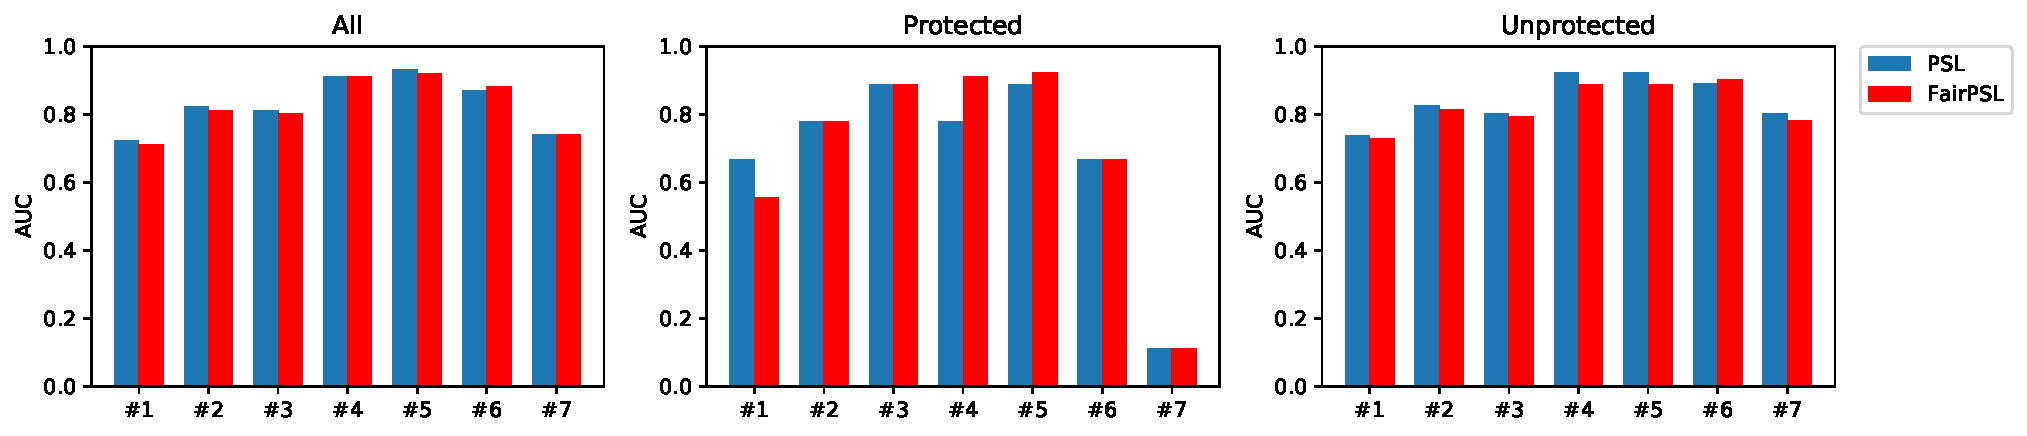
\includegraphics[width=\textwidth]{figs/roc.pdf}
    \caption{\small AUC score of predictions for truth values of unknown atoms \textit{ToPromote(e)} using MAP inference of PSL and FairPSL with $\delta$-fairness constraints $RD$ with $\delta=0.001$.}
    \label{fig:accuracy}
\end{figure}

According to Figure~\ref{fig:accuracy}, the results of both PSL and FairPSL in all seven datasets are close to each other. Note that although fairness may impose a cost in terms of overall accuracy, FairPSL often improves the accuracy of the protected class. Sometimes the overall predictions of FairPSL are even slightly better than PSL (e.g., dataset 6 and 7). As expected, the accuracy of the fourth setting where the opinions are unbiased are similar in both PSL and FairPSL. We observe that prediction of MAP inference for both FairPSL and PSL are similar, thus, in these settings at least, FairPSL guarantees fairness without hurting accuracy. Further investigation is required on the effect of the various ranges of discrimination (i.e., $\theta_1$, $\theta_2$, $\theta_3$, $\theta_4$) on the prediction results of FairPSL.



We also generate various types of organizations in which labels are not uniformly distributed, e.g., one population only occurs at the bottom levels of an organization. While we did not observe any differences in the behavior of our method with respect to accuracy and fairness measure, we found that the degree of discrimination is higher in such organizations. Further investigations on the structure of an organization on discrimination is an interesting direction for future research. 

\section{Conclusion and Future Directions}
\label{sec:conclusion}
Many applications of AI and machine learning affect peoples' lives in important ways. While there is a growing body of work on fairness in AI and ML, it assumes an individualistic notion of fairness.   In this paper, we have proposed a general framework for relational fairness which includes both a rich language for defining discrimination patterns and an efficient algorithm for performing inference subject to fairness constraints. We show our approach enforces fairness guarantees while preserving the accuracy of the predictions. 

There are many avenues for expanding on this work. For example, here we assumed that the discriminative pattern is given, however an automatic mechanism to extract discriminatory situations hidden in a large amount of decision records is an important and required task. Discrimination discovery has been studied for attribute-based fairness~\cite{pedreschi2013discovery}. An interesting next step is discrimination pattern discovery in relational data.

\section*{Acknowledgements}
This work is supported by the National Science Foundation under Grant Numbers CCF-1740850 and IIS-1703331. Golnoosh Farnadi and Behrouz Babaki are  supported by postdoctoral scholarships from IVADO through the Canada First Research Excellence Fund (CFREF) grant.

\begin{thebibliography}{10}
\itemsep=1pt 
\begin{small}

\bibitem{EUlaw}
European union legislation. (a) racial equality directive, 2000; (b) employment
  equality directive, 2000; (c) gender employment directive, 2006; (d) equal
  treatment directive (proposal), 2008.

\bibitem{UKlaw}
{UK} legislation. (a) sex discrimination act, 1975, (b) race relation act,
  1976.

\bibitem{USlaw}
United nations legislation. (a) universal declaration of human rights, 1948,
  (c) convention on the elimination of all forms of racial discrimination,
  1966, (d) convention on the elimination of all forms of discrimination
  against women, 1979.

\bibitem{alshukaili:iswc16}
Duhai Alshukaili, Alvaro A.~A. Fernandes, and Norman~W. Paton.
\newblock Structuring linked data search results using probabilistic soft
  logic.
\newblock In {\em International Semantic Web Conference {(1)}}, volume 9981 of
  {\em Lecture Notes in Computer Science}, pages 3--19, 2016.

\bibitem{bach:jmlr17}
Stephen~H. Bach, Matthias Broecheler, Bert Huang, and Lise Getoor.
\newblock Hinge-loss markov random fields and probabilistic soft logic.
\newblock {\em Journal of Machine Learning Research}, 18:109:1--109:67, 2017.

\bibitem{barocas2016big2}
Solon Barocas and Andrew~D Selbst.
\newblock Big data's disparate impact.
\newblock {\em California Law Review}, 104:671, 2016.

\bibitem{boyd2014networked}
Danah Boyd, Karen Levy, and Alice Marwick.
\newblock The networked nature of algorithmic discrimination.
\newblock In {\em Data and discrimination: Collected essays}, pages 53--57.
  2014.

\bibitem{brewer1979group}
Marilynn~B Brewer.
\newblock In-group bias in the minimal intergroup situation: A
  cognitive-motivational analysis.
\newblock {\em Psychological bulletin}, 86(2):307, 1979.

\bibitem{brewer2007social}
Marilynn~B Brewer.
\newblock The social psychology of intergroup relations: Social categorization,
  ingroup bias, and outgroup prejudice.
\newblock {\em Social Psychology: Handbook of Basic Principles}, 2007.

\bibitem{chouldechova2017fair2}
Alexandra Chouldechova.
\newblock Fair prediction with disparate impact: {A} study of bias in
  recidivism prediction instruments.
\newblock {\em CoRR}, abs/1703.00056, 2017.

\bibitem{dwork2012fairness3}
Cynthia Dwork, Moritz Hardt, Toniann Pitassi, Omer Reingold, and Richard~S.
  Zemel.
\newblock Fairness through awareness.
\newblock In {\em {ITCS}}, pages 214--226. {ACM}, 2012.

\bibitem{ebrahimi:emnlp16}
Javid Ebrahimi, Dejing Dou, and Daniel Lowd.
\newblock Weakly supervised tweet stance classification by relational
  bootstrapping.
\newblock In {\em {EMNLP}}, pages 1012--1017. The Association for Computational
  Linguistics, 2016.

\bibitem{farnadi2018fairness}
Golnoosh Farnadi, Behrouz Babaki, and Lise Getoor.
\newblock Fairness in relational domains.
\newblock In {\em AAAI/ACM Conference on AI, Ethics, and Society (AIES)}, pages
  108--114. ACM, 2018.

\bibitem{feldman2015certifying2}
Michael Feldman, Sorelle~A. Friedler, John Moeller, Carlos Scheidegger, and
  Suresh Venkatasubramanian.
\newblock Certifying and removing disparate impact.
\newblock In {\em {KDD}}, pages 259--268. {ACM}, 2015.

\bibitem{getoor2007introduction}
Lise Getoor and Ben Taskar.
\newblock {\em {Introduction to Statistical Relational Learning}}.
\newblock MIT press Cambridge, 2007.

\bibitem{hardt2016equality3}
Moritz Hardt, Eric Price, and Nati Srebro.
\newblock Equality of opportunity in supervised learning.
\newblock In {\em {NIPS}}, pages 3315--3323, 2016.

\bibitem{kamishima2011fairness}
Toshihiro Kamishima, Shotaro Akaho, and Jun Sakuma.
\newblock Fairness-aware learning through regularization approach.
\newblock In {\em ICDMW}, pages 643--650. {IEEE} Computer Society, 2011.

\bibitem{kouki:recsys15}
Pigi Kouki, Shobeir Fakhraei, James~R. Foulds, Magdalini Eirinaki, and Lise
  Getoor.
\newblock Hyper: {A} flexible and extensible probabilistic framework for hybrid
  recommender systems.
\newblock In {\em RecSys}, pages 99--106. {ACM}, 2015.

\bibitem{counterfactualfairness}
Matt~J. Kusner, Joshua~R. Loftus, Chris Russell, and Ricardo Silva.
\newblock Counterfactual fairness.
\newblock In {\em {NIPS}}, pages 4069--4079, 2017.

\bibitem{Pedreschi:2012}
Dino Pedreschi, Salvatore Ruggieri, and Franco Turini.
\newblock A study of top-k measures for discrimination discovery.
\newblock In {\em {SAC}}, pages 126--131. {ACM}, 2012.

\bibitem{pedreschi2013discovery}
Dino Pedreschi, Salvatore Ruggieri, and Franco Turini.
\newblock The discovery of discrimination.
\newblock In {\em Discrimination and Privacy in the Information Society},
  volume~3 of {\em Studies in Applied Philosophy, Epistemology and Rational
  Ethics}, pages 91--108. Springer, 2013.

\bibitem{ridgeway2004unpacking}
Cecilia~L Ridgeway and Shelley~J Correll.
\newblock Unpacking the gender system: A theoretical perspective on gender
  beliefs and social relations.
\newblock {\em Gender \& society}, 18(4):510--531, 2004.

\bibitem{sridhar:bioinformatics16}
Dhanya Sridhar, Shobeir Fakhraei, and Lise Getoor.
\newblock A probabilistic approach for collective similarity-based drug-drug
  interaction prediction.
\newblock {\em Bioinformatics}, 32(20):3175--3182, 2016.

\bibitem{verma2018fairness2}
Sahil Verma and Julia Rubin.
\newblock Fairness definitions explained.
\newblock In {\em 2018 IEEE/ACM International Workshop on Software Fairness
  (FairWare)}, pages 1--7. IEEE, 2018.

\bibitem{west2014exploiting}
Robert West, Hristo~S. Paskov, Jure Leskovec, and Christopher Potts.
\newblock Exploiting social network structure for person-to-person sentiment
  analysis.
\newblock {\em {TACL}}, 2:297--310, 2014.

\bibitem{zafar2017parity}
Muhammad~Bilal Zafar, Isabel Valera, Manuel Gomez{-}Rodriguez, Krishna~P.
  Gummadi, and Adrian Weller.
\newblock From parity to preference-based notions of fairness in
  classification.
\newblock In {\em {NIPS}}, pages 228--238, 2017.

\bibitem{zemel2013learning}
Richard~S. Zemel, Yu~Wu, Kevin Swersky, Toniann Pitassi, and Cynthia Dwork.
\newblock Learning fair representations.
\newblock In {\em {ICML} {(3)}}, volume~28 of {\em {JMLR} Workshop and
  Conference Proceedings}, pages 325--333. JMLR.org, 2013.

\end{small}
\end{thebibliography}

\end{document}

\end{article}


\begin{article}
{External vs. Internal: An Essay on  Machine Learning Agents for  Autonomous Database Management Systems}
{Andrew Pavlo, Matthew Butrovich, Ananya Joshi, Lin Ma, Prashanth 
Menon, Dana Van Aken, Lisa Lee, Ruslan Salakhutdinov}
\graphicspath{{submissions/selfdriving/}}
%\documentclass[11pt,dvipdfm]{article}
\documentclass[11pt]{article}
\usepackage{deauthor,times,graphicx} %required
\usepackage{amsmath,amssymb}
\usepackage{multirow}
\usepackage{algorithm}
\usepackage{algpseudocode}
\usepackage{todonotes}
\usepackage{url}

% \graphicspath{{farnadi/}}

\newtheorem{mydef}{\textbf{Definition}}
\newtheorem{myex}{\textbf{Example}}
\newtheorem{mytheorem}{\textbf{Theorem}}


\begin{document}

\title{A Declarative Approach to Fairness in Relational Domains}
\author{Golnoosh Farnadi$^{1,2}$, Behrouz Babaki$^1$, Lise Getoor$^3$\\
$^1$Polytechnique Montr\'{e}al, $^2$ Mila, $^3$ UC Santa Cruz \\
farnadig@mila.quebec, behrouz.babaki@polymtl.ca, getoor@soe.ucsc.edu}

\maketitle

\begin{abstract}
AI and machine learning tools are being used with increasing frequency for decision making in domains that affect peoples' lives such as employment, education, policing and %loan approval
financial qualifications. These uses raise concerns about biases of algorithmic discrimination and have motivated the development of fairness-aware machine learning. However, existing fairness approaches are based solely on attributes of individuals. In many cases, discrimination is much more complex, and taking into account the social, organizational, and other connections between individuals is important. We introduce new notions of fairness that are able to capture the relational structure in a domain. We use first-order logic to provide a flexible and expressive language for specifying complex relational patterns of discrimination. Furthermore, we extend an existing statistical relational learning framework, probabilistic soft logic~(PSL), to incorporate our definition of relational fairness. We refer to this fairness-aware framework FairPSL. FairPSL makes use of the logical definitions of fairnesss but also supports a probabilistic interpretation. In particular, we show how to perform maximum a posteriori~(MAP) inference by exploiting probabilistic dependencies within the domain while avoiding violations of fairness guarantees. Preliminary empirical evaluation shows that we are able to make both accurate and fair decisions.
\end{abstract}

\section{Introduction}
\label{sec:introduction}

Over the past few years, AI and machine learning have become essential components in operations that drive the modern society, e.g., in financial, administrative, and educational spheres. \emph{Discrimination} happens when qualities of individuals which are not relevant to the decision making process influence the decision. Delegating decision making to an automated process raises questions about discriminating against individuals with certain traits based on biases in the data. This is especially important when the decisions have the potential to impact the lives of individuals, for example, the decisions on granting loans, assigning credit, and employment. 

\emph{Fairness} is defined as the absence of discrimination in a decision making process. The goal of \emph{fairness-aware} machine learning is to ensure that the decisions made by an algorithm do not discriminate against a population of individuals~\cite{feldman2015certifying2,boyd2014networked,hardt2016equality3}. Fairness has been well studied in the social sciences and legal scholarship (for an in-depth review see~\cite{barocas2016big2}), and there is emerging work on fairness-aware ML within the AI and computer science communities. For example, fairness through awareness/Lipschitz property~\cite{dwork2012fairness3}, individual fairness~\cite{zemel2013learning}, statistical parity/group fairness~\cite{kamishima2011fairness}, counterfactual fairness~\cite{counterfactualfairness}, demographic parity/disparate impact~\cite{feldman2015certifying2,chouldechova2017fair2}, preference-based fairness~\cite{zafar2017parity}, and equality of opportunity~\cite{hardt2016equality3}.

The existing work in fairness-aware machine learning is based on a definition of discrimination where a decision is influenced by an \emph{attribute} of an individual. An attribute value upon which discrimination is based (such as gender, race, or religion) is called a \emph{sensitive attribute}. The sensitive attribute defines a population of vulnerable individuals known as the \emph{protected group}. A fair decision-making process treats the protected group the same as the \emph{unprotected group}. 

However, in many social contexts, discrimination is the result of complex interactions and can not be described solely in terms of attributes of an individual. For example, consider an imaginary scenario in an organization in which younger female workers who have older male supervisors have lower chances of promotion than their male counterparts.\footnote{Of course, many other patterns may be possible: female bosses may promote female subordinates and discriminate against male workers, or male bosses may promote female employees.  Our goal is to provide a general framework which is able to describe arbitrarily complex discrimination patterns.} 
 This discrimination pattern involves two attributes of the individual (gender and age), a relationship with another individual (supervisor), and two attributes of the second individual. Addressing such complex cases poses two challenges. First, the concepts of discrimination and fairness need to be extended to capture not only attributes of individuals but also the relationships between them. Second, a process is required that ensures that fair decisions are made about individuals who are affected by such patterns. In this paper we address both of these challenges.
We use first-order logic (FOL) to extend the notion of fairness to the relational setting. FOL is an expressive representation for relational problems which is also widely used for learning in relational domains. Moreover, we extend an existing framework for statistical relational learning~\cite{getoor2007introduction} called probabilistic soft logic (PSL)\footnote{http://psl.linqs.org/}~\cite{bach:jmlr17}. PSL combines logic and probability for learning and reasoning over uncertain relational domains. One of the most common reasoning tasks in PSL is called maximum a posteriori (MAP) inference, which is performed by finding the most probable truth values for unknowns over a set of given evidence. We develop a new MAP inference algorithm which is able to maximize the a posteriori values of unknown variables \emph{subject to} fairness guarantees. An early version of this paper which this work builds upon and extends appeared in~\cite{farnadi2018fairness}.

\looseness-1
Our contributions are as follows: 1) we propose fairness-aware machine learning for the relational setting; 2) we extend PSL into a fairness-aware framework called FairPSL which can represent the logical definition of fairness; 3) we develop a new MAP inference algorithm which is able to maximize the posteriori values of unknown variables \emph{subject to} fairness guarantees; 4) we empirically evaluate our proposed framework on synthetic data. 

\section{Motivation}
\label{sec:motivation}

Discrimination in social contexts have been studied in the field of social psychology~\cite{brewer2007social,brewer1979group,ridgeway2004unpacking}. There is a large literature on various aspects of relational bias in social contexts such as \emph{in-group-out-group bias}, \emph{gender bias}, and \emph{ethnicity-based favoritism} that can result in discrimination. 
As an example, consider gender bias in the workplace that reflects stereotypically masculine criteria and male-based favoritism. Such gender bias 
typically places women in lower positions and negatively impacts their opportunities. Further, lack of women in leadership positions may affect the promotion of women and results in a glass ceiling that keeps women from rising beyond a certain level in the hierarchy. This scenario shows that considering  protected attributes such as gender is not always sufficient to detect the source of bias and avoid discrimination, one also has to consider the relational information, in this case the organization hierarchy. Note that this can be generalized to any ingroup/outgroup scenario where the sensitive attribute could be race, religion, age, marital-status, etc.

The existing work on designing fair algorithms in machine learning exclusively focuses on \emph{attribute-based fairness}, which is based on the following assumptions: First, there is an assumption that the individuals (sometimes referred to as units or entities) are independent and described by simple attribute vectors. Second, the group for which one wishes to ensure fairness (known as the \emph{protected group}) is defined on the basis of some attribute values. Finally, there is a decision that is associated with each individual, and the goal is to ensure that members of the protected group are subject to a fair decision (we discuss different fairness measures in Section~\ref{sec:fairnessmeasure}).  We illustrate  attribute-based fairness in the following example. 

\begin{myex}[Loan Processing]
\label{ex:loan}
A bank bases its decisions about granting a loan on attributes of the applicant. The goal is to decide whether to grant a loan to an applicant using a predictive model. The bank needs to ensure that the obey fair lending practices and ensure that gender, race, sexual orientation of applicants has no influence on the decision. In this scenario, the protected group is the historically disadvantaged applicants.  
\end{myex}
The current fairness-aware machine learning techniques are not capable of modeling relations and hence cannot be used to make the decision making model fair. However, in many decision making scenarios, especially in social and organizational settings, the domain is relational, and the protected group itself might be best represented using a relational definition. We illustrate this setting in the following scenario:
\begin{myex}[Performance Review]
\label{ex:review}
Consider an organization where decisions about the promotion of employees is based on two criteria: 1) an objective performance measure, and 2) the opinion of their direct and indirect managers above them. The opinions are inferred from the performance reviews which are collected periodically. Not every manager can submit a review for all its subordinates, this is especially the case for top-level managers who have a large number of subordinates. Hence, the opinions of managers are collectively inferred from the opinions of their sub-ordinates. However, some employees may be biased, and judge other employees unfavorably, by favoring employees who are similar to themselves (same gender, race, religion, etc.) over employees who are dissimilar. The organization needs to ensure that promotion of employees do not have any relational bias caused by in-group-out-group favoritism.

\end{myex}
Example~\ref{ex:review} describes a prediction problem over a database that consists of relations between employees. Such prediction tasks are best handled by techniques from the relational learning domain. To ensure fair prediction in such settings, we need to extend the notion of \emph{attribute-based fairness} to \emph{relational fairness}. Throughout this paper, we use the performance review problem as a running example for relational fairness.

\section{Fairness Formalism}
\label{sec:formulation}

A representation that can describe different types of entities and different relationships between them is called relational. In this section, we use first-order logic to define relational fairness. We employ first-order logic as an expressive representation formalism which can represent objects and complex relationships between them. We start by defining an atom:

\begin{mydef}[Atom]
An atom is an expression of the form $P(a_1, a_2, \ldots, a_n)$ where each argument $a_1, a_2,$ $\ldots,$ $a_n$ is either a constant or a variable. The finite set of all possible substitutions of a variable to a constant for a particular variable $a$ is called its \textit{domain} $D_{a}$. If all variables in $P(a_1, a_2, \ldots, a_n)$ are substituted by some constant from their respective domain, then we call the resulting atom a \textit{ground atom}. 
\end{mydef}

\begin{myex}
In our loan processing problem (Example~\ref{ex:loan}), we can represent applicants' attributes by atoms. For instance, atom $Female(v)$ indicates whether or not applicant $v$ is female. Similarly, we can represent relations with atoms. In the performance review problem in Example~\ref{ex:review} the atom $Manager(m,e)$ indicates whether or not employee $m$ is a direct or indirect manager of employee $e$.
\end{myex}

The relational setting provides the flexibility to express complex definitions with formulae.

\begin{mydef}[Formula] 
A formula is defined by induction: every atom is a formula. If $\alpha$ and $\beta$ are formulae, then $\alpha \vee \beta$, $\alpha \wedge \beta$, $\neg \alpha$, $\alpha \rightarrow \beta$ are formulae. If $x$ is a variable and $\alpha$ is a formula, then the quantified expressions of the form $\exists x$ $\alpha$ and $\forall x$ $\alpha$ are formulae.    
\end{mydef}

To characterize groups of individuals based on a formula, we define the notion of \emph{population}.

\begin{mydef}[Population]
We denote formula $F$ which has only one free variable $v$ (i.e., other variables in $F$ are quantified) by $F[v]$. The population defined by $F[v]$ is the set of substitutions of $v$ for which $F[v]$ holds.   
\end{mydef}


\begin{myex}
\label{ex:disformula}
Consider the formula $F[v] := \forall u, \, \textit{Manager}(u,v) \rightarrow \neg \textit{SameGroup}(u, v)$. The population specified by this formula is the set of individuals all of whose managers belong to a group different from theirs. 
\end{myex}

The truth value of a formula is derived from the truth value of atoms that it comprises, according to the rules of logic. Each possible assignment of truth values to ground atoms is called an \emph{interpretation}. 


\begin{mydef}[Interpretation]
An interpretation $I$ is a mapping that associates a truth value $I(P)$ to each ground atom $P$. For Boolean truth values, $I$ associates true to 1 and false to 0 truth values. For soft logic (see Definition~\ref{def:softlogic}) $I$ maps each ground atom $P$ to a truth value in interval $[0, 1]$.
\end{mydef}

In attribute-based fairness, it is assumed that there is a certain attribute of individuals, i.e, the sensitive attribute,  that we do not want to affect a decision. Gender, race, religion and marital status are examples of sensitive attributes. Discrimination has been defined in social science studies as a treatment in favor or against a group of individuals given their sensitive attribute. This group of individuals is the protected group. 

In a relational setting, both the sensitive attributes of an individual and their participation in various relations may have an undesired effect on the final decision. We characterize the protected group in a relational setting by means of a population. In practice, we are often interested in maintaining fairness for a specific population such as applicants, students, employees, etc. This population is then partitioned into the protected and unprotected groups. We define a \emph{discriminative pattern} which is a pair of formulae to capture these groups: 1) $F_1[v]$: to specify the difference between the protected and unprotected groups and 2) $F_2[v]$: to specify the population over which we want to maintain fairness. 

\begin{mydef}[Discriminative pattern]
A discriminative pattern is a pair $\textit{DP}[v]:=(F_1[v], F_2[v])$ , where $F_1[v]$ and $F_2[v]$ are formulae.
\end{mydef}

\begin{myex}
\label{ex:pattern}
The two formulae in the discrimination pattern $\textit{DP}[v]:= \big((\forall u, \,  \textit{Manager}(u,v) \rightarrow  \neg \textit{SameGroup}(u, v)),$ $\textit{Employee}(v)\big)$ specify two populations, namely all employees and those employees who belong to a group different from their managers.
\end{myex}

Given the definition of the discriminative pattern, we have a rich language to define the scope of the protected and unprotected groups in a relational setting.

\begin{mydef}[Protected group] Given an interpretation $I$, the protected group is a population of the form:
{$$PG :=\{ v : F_1[v] \wedge F_2[v]\}$$}
which is defined as the set of all instances hold for variable $v$ for which $F_1[v] \wedge F_2[v]$ is true under interpretation $I$, that is, $I(F_1[v] \wedge F_2[v]) = 1$. 
Similarly, the \emph{unprotected group} is a population of the form: 
{$$UG := \{ v : \neg F_1[v] \wedge  F_2[v]\}$$}
which is defined as the set of all instances hold for variable $v$ 
for which $I(\neg F_1[v] \wedge F_2[v]) = 1$. 
\end{mydef}

\begin{myex}
The protected group of the discrimination pattern specified in Example~\ref{ex:pattern} is {$PG := \big\{ v : \big(\forall u, \,$ $ \textit{Manager}(u, v) \rightarrow \neg \textit{SameGroup}(u, v)\big) \wedge \textit{Employee}(v) \big\}$} and the unprotected group is {$UG :=  \big\{ v:  \big(\exists u, \, \textit{Manager}(u,v) \wedge \textit{SameGroup}(u, v)\big) \wedge \textit{Employee}(v) \big\}$}. This means our protected group is the set of employees belonging to a group different from their managers,
and our unprotected group consists of other employees. 
\end{myex}

Discrimination is defined in terms of a treatment or decision that distinguishes between the protected and unprotected groups. Here we define the \emph{decision} atom.
\begin{mydef}[Decision atom] A decision atom $d(v)$ is an atom containing exactly one variable $v$ that specifies a decision affecting the protected group which is defined either by law or end-user.
\end{mydef}
\begin{myex}
The decision atom ${\textit ToPromote}(v)$ indicates whether or not $v$ receives a promotion.
\end{myex}

Note that the fairness formulation in this section is designed for the relational setting, however relational fairness subsumes the attribute-based fairness such that: a sensitive attribute is defined by an atom with one argument and $F_2[v]$ in discrimination pattern is $\textit{Applicant}(v)$. For example, discrimination pattern of our loan processing problem in Example~\ref{ex:loan} is of the form $\textit{DP} := ( \textit{Female}(v), \textit{Applicant}(v))$ that denotes female applicants as the protected group (i.e., $PG :=  \{ v: \textit{Female}(v) \}$) and male applicants as the unprotected group (i.e., $UG := \{ v: \neg \textit{Female}(v)\}$).


\section{Fairness Measures}
\label{sec:fairnessmeasure}

Over the past few years, many fairness measures have been introduced~\cite{verma2018fairness2}. An important class of these measures are \emph{group fairness} measures which quantify the inequality between different subgroups. Some of the most popular measures in this class include \emph{equal opportunity}, \emph{equalized odds}, and \emph{demographic parity}~\cite{hardt2016equality3}. In this paper we restrict our focus to the latter. In an attribute-value setting, demographic parity means that the decision should be independent of the protected attributes. Assume that binary variables $A$ and $C$ denote the decision and protected attributes, and the preferred value of $A$ is one. Demographic parity requires that:

\begin{equation*}
    P(A=1 | C=0) = P(A=1 | C=1)
\end{equation*}

We will now generalize this measure to the relational setting using the notations defined in Section~\ref{sec:formulation}. Let $a$ and $c$ denote the counts of denial (i.e., negative decisions) for protected and unprotected groups, and $n_{1}$ and $n_{2}$ denote their sizes, respectively. Given the decision atom $d(v)$, discriminative pattern $\textit{DP}(F_1[v], F_2[v])$, and interpretation $I$, these counts are computed by the following equations: 
{
\begin{flalign}
    & a \equiv \sum_{v \in D_v} I\big( \neg d(v) \wedge  F_1[v] \wedge F_2[v]) \label{eq:a}\\
    & c \equiv \sum_{v \in D_v} I\big( \neg d(v) \wedge  \neg F_1[v] \wedge  F_2[v]) \label{eq:c}\\
    & n_{1} \equiv \sum_{v \in D_v} I\big(F_1[v] \wedge F_2[v]) \label{eq:n1}\\
    & n_{2} \equiv \sum_{v \in D_v} I\big(\neg F_1[v] \wedge  F_2[v]) \label{eq:n2}
\end{flalign}}
The proportions of denying for protected and unprotected groups are $p_1 = \frac{a}{n_1}$ and $p_2 = \frac{c}{n_2}$, respectively. There are a number of data-driven measures~\cite{Pedreschi:2012} which quantify demographic disparity and can be defined in terms of $p_1$ and $p_2$:
\begin{itemize}
    \item \textbf{Risk difference}: $RD = p_1 - p_2$, also known as absolute risk reduction. 
    \item \textbf{Risk Ratio}: $RR = \frac{p_1}{p_2}$, also known as relative risk. 
    \item \textbf{Relative Chance}: $RC = \frac{1 - p_1}{1 - p_2}$ also, known as selection rate.
\end{itemize}
These measures have been used in the legal systems of European Union, UK, and US~\cite{EUlaw,UKlaw,USlaw}. Notice that RR is the ratio of the proportion of benefit denial between the protected and unprotected groups, while RC is the ratio of the proportion of benefit granted. Finally, we introduce the notion of $\delta$-fairness.

\begin{mydef}[$\delta$-fairness]
If a fairness measure for a decision making process falls within some $\delta$-window, then the process is \emph{$\delta\text{-fair}$}. Given $0 \leq \delta \leq 1$, the  $\delta$-windows for measures RD/RR/RC are defined as:
{\begin{flalign*}
	     - \delta \leq &RD \leq \delta \\
	     1- \delta \leq &RR \leq 1+ \delta\\
	     1- \delta \leq &RC \leq 1+ \delta
	\end{flalign*}}
\end{mydef}

To overcome the limitations of attribute-based fairness, we introduce a new statistical relational learning~(SRL) framework~\cite{getoor2007introduction} suitable for modelling fairness in relational domain. In the next section, we review probabilistic soft logic~(PSL). We then extend PSL with the definition of relational fairness introduced above in Section~\ref{sec:fairMAP}. Our fairness-aware framework, ``FairPSL'', is the first SRL framework that performs fair inference. 

\section{Background: Probabilistic Soft Logic}
\label{sec:psl}

In this section, we review the syntax and semantics of PSL, and in the next section we extend MAP inference in PSL with fairness constraints to define MAP inference in FairPSL.

PSL is a probabilistic programming language for defining hinge-loss Markov random fields~\cite{bach:jmlr17}. Unlike other SRL frameworks whose atoms are Boolean, atoms in PSL can take continuous values in the interval $[0,1]$. PSL is an expressive modeling language that can incorporate domain knowledge with first-order logical rules and has been used successfully in various domains, including bioinformatics~\cite{sridhar:bioinformatics16}, recommender systems~\cite{kouki:recsys15}, natural language processing~\cite{ebrahimi:emnlp16}, information retrieval~\cite{alshukaili:iswc16}, and social network analysis~\cite{west2014exploiting}, among many others. 
 
A PSL model is defined by a set of first-order logical rules called \emph{PSL rules}.

\begin{mydef} [PSL rule] a PSL rule $r$ is an expression of the form:
{\begin{equation}
\lambda_{r}: T_1 \land T_2 \land \ldots \land T_w \rightarrow H_1 \vee H_2 \vee \ldots \vee H_l
\end{equation}}

where { $T_1, T_2, \ldots, T_w, H_1, H_2, \ldots, H_l$} are atoms or negated atoms and { $\lambda_{r} \in \mathbb{R}^{+} \cup \infty$} is the weight of the rule $r$.  We call { $T_1 \land T_2 \land \ldots \land T_w$} the body of $r$ ($r_{body}$), and { $H_1 \vee H_2 \vee \ldots \vee H_l$} the head of $r$ ($r_{head}$).
\end{mydef}


Since atoms in PSL take on continuous values in the unit interval $[0,1]$, next we define soft logic to calculate the value of the PSL rules under an interpretation $I$.

\begin{mydef}[Soft logic]
\label{def:softlogic}
The ({$\tilde{\wedge}$}) and ({$\tilde{\vee}$}) and negation ({$\tilde{\neg}$}) are defined as follows. For {$m, n \in [0,1]$} we have: {$m \tilde{\wedge} n = \max(m+n -1, 0)$}, {$m \tilde{\vee} n = \min(m+n , 1)$} and {$\tilde{\neg} m = 1 - m$}. The $\, \tilde{} \,$ indicates the relaxation over Boolean values.
\end{mydef}

The probability of truth value assignments in PSL is determined by the rules' \emph{distance to satisfaction}.

\begin{mydef}[The distance to satisfaction]
The distance to satisfaction $d_{r}(I)$ of a rule $r$ under an interpretation $I$ is defined as:
{
\begin{equation}
d_{r}(I) = \max\{0, I(r_{body})-I(r_{head})\}
\end{equation}}
\end{mydef}

By using Definition~\ref{def:softlogic}, one can show that the closer the interpretation of a grounded rule $r$ is to 1, the smaller its distance to satisfaction. A PSL model induces a distribution over interpretations $I$. Let $R$ be the set of all grounded rules, then the probability density function is:
{
\begin{equation}
f(I) ={\frac{1}{Z}} \exp[-\sum_{r\in R} \lambda_{r}(d_{r}(I))^p]
\label{eq:potential}
\end{equation}
}
\noindent where { $\lambda_{r}$} is the weight of rule $r$, {
$Z = \int_{I} \exp[ -\sum_{r\in R} \lambda_{r}(d_{r}(I))^p]$
} is a normalization constant, and { $p \in \{1,2\}$} provides a choice of two different loss functions, $p=1$ (i.e., linear), and $p=2$ (i.e, quadratic). These probabilistic models are instances of hinge-loss Markov random fields~(HL-MRF)~\cite{bach:jmlr17}. The goal of maximum a posteriori (MAP) inference is to find the most probable truth assignments $I_{\textit{MPE}}$ of unknown ground atoms given the evidence which is defined by the interpretation $I$. Let $X$ be all the evidence, i.e., $X$ is the set of ground atoms such that $\forall x \in X, I(x)$ is known, and let $Y$ be the set of ground atoms such that $\forall y \in Y, I(y)$ is unknown. Then we have
{
\begin{equation}
I_{\textit{MAP}}(Y) = \textit{arg}\max_{I(Y)} P(I(Y)|I(X))
\end{equation}}
Maximizing the density function in Equation~\ref{eq:potential} is equivalent to minimizing the weighted sum of the distances to satisfaction of all rules in PSL. 

\begin{table*}[t]
    \centering
    \begin{tabular}{|lll|}
    \hline
    &&\\
    $R1$ & $\lambda_1$ &: $\textit{IsQualified}(e) \rightarrow \textit{HighPerformance}(e)$ \\
    $R2$ & $\lambda_1$ &: $\neg \textit{IsQualified}(e) \rightarrow \neg \textit{HighPerformance}(e)$ \\
    $R3$ & $\infty$ &: $\textit{PositiveReview}(e1, e2) \rightarrow \textit{PositiveOpinion}(e1, e2)$ \\
    $R4$ & $\infty$ &: $\neg \textit{PositiveReview}(e1, e2) \rightarrow \neg \textit{PositiveOpinion}(e1, e2)$ \\
    $R5$ & $\lambda_1$ &: $\textit{PositiveOpinion}(e1, e2) \wedge \textit{Manager}(m, e1) \rightarrow \textit{PositiveOpinion}(m, e2)$ \\
    $R6$ & $\lambda_1$ &: $\neg \textit{PositiveOpinion}(e1, e2) \wedge \textit{Manager}(m, e1) \rightarrow \neg \textit{PositiveOpinion}(m, e2)$ \\
    $R7$ & $\lambda_1$ &: $\textit{PositiveOpinion}(m, e) \wedge \textit{Manager}(m, e) \rightarrow \textit{IsQualified}(e)$ \\
    $R8$ & $\lambda_1$ &: $\neg \textit{PositiveOpinion}(m, e) \wedge \textit{Manager}(m, e) \rightarrow \neg \textit{IsQualified}(e)$ \\
    $R9$ &  $\lambda_1$ &: $\neg \textit{ToPromote}(e)$\\
    $R10$ & $\infty$ &: $\textit{IsQualified}(e) \rightarrow \textit{ToPromote}(e)$ \\
    $R11$ & $\infty$ &: $\neg \textit{IsQualified}(e) \rightarrow \neg \textit{ToPromote}(e)$ \\
    &&\\
    \hline
    \end{tabular}
    \caption{\small A simplified PSL model for the \emph{Performance Reviewing} problem}
    \label{tab:pslmodel}
\end{table*}

\begin{myex}
\label{ex:pslmodel}
The simplified PSL model for the performance reviewing problem in Example\ref{ex:review} is given in Table~\ref{tab:pslmodel}. The goal of MAP inference for this problem is to infer employees to promote. We simplified the model by assigning the same weight to all soft rules (i.e., $\lambda_i= 1$ where $i=\{1,2,5,6,7,8,9\}$). Below we explain the meaning of each rule in the model.

Rule $R1$ indicates that qualified employees have high performance and similarly rule $R2$ expresses that a negative qualification of employees is derived from their low performance. Rules $R5$ and $R6$ presents the propagation of opinion from bottom to top of the organizational hierarchy, i.e., managers have similar opinions towards employees given the opinions of their sub-ordinate managers. And rules $R7$ and $R8$ indicate that the positive/negative opinion of direct/indirect managers derive from the qualification of an employee. Rule $R9$ indicates the prior that not all employees get promoted. We also have four hard constraints (i.e., rules $R3$, $R4$, $R10$ and $R11$) where the weight of the rules are $\infty$. Rules $R3$ and $R4$ indicate that submitted positive/negative reviews should reflect positive/negative opinions. And two rules $R10$ and $R11$ show that a highly qualified employee should get promoted. 
\end{myex}

\section{Fairness-aware PSL (FairPSL)}
\label{sec:fairMAP}

The standard MAP inference in PSL aims at finding values that maximize the conditional probability of unknowns. Once a decision is made according to these values, one can use the fairness measure to quantify the degree of discrimination. A simple way to incorporate fairness in MAP inference is to add the $\delta$-fairness constraints to the corresponding optimization problem.   

Consider risk difference, $\textit{RD}$, where $\textit{RD} \equiv \frac{\mathbf{a}}{n_1} - \frac{\mathbf{c}}{n_2}$. The $\delta$-fairness constraint $-\delta \leq \textit{RD} \leq \delta$ can be encoded as the following constraints:
{\begin{align}
    & n_2 \mathbf{a} - n_1 \mathbf{c} - n_1 n_2 \delta \leq 0 \label{eq:RD1}\\
    & n_2 \mathbf{a} - n_1 \mathbf{c} + n_1 n_2 \delta \geq 0
\end{align}}
Similarly, from $\textit{RR} \equiv \frac{\mathbf{a} / n_1}{\mathbf{c} / n_2}$ and the $\delta$-fairness constraint $1 - \delta \leq \textit{RR} \leq 1 + \delta$ we obtain:
{\begin{align}
    & n_2 \mathbf{a} - (1 + \delta) n_1 \mathbf{c} \leq 0 \\
    & n_2 \mathbf{a} - (1 - \delta) n_1 \mathbf{c} \geq 0
\end{align}}
And finally, $\textit{RC} \equiv \frac{1 - \mathbf{a} / n_1}{1 - \mathbf{c} / n_2}$ and the $\delta$-fairness constraint $1 - \delta \leq \textit{RC} \leq 1 + \delta$ gives:
{ \begin{align}
    & - n_2 \mathbf{a} + (1 + \delta) n_1 \mathbf{c} - \delta n_1 n_2 \leq 0 \\
    & - n_2 \mathbf{a} + (1 - \delta) n_1 \mathbf{c} + \delta n_1 n_2 \geq 0 \label{eq:RC2}
\end{align}}
A primary advantage of PSL over similar frameworks is that its MAP inference task reduces to a convex optimization problem which can be solved in polynomial time. To preserve this advantage, we need to ensure that the problem will remain convex after the addition of $\delta$-fairness constraints. 

\begin{mytheorem}
The following condition is sufficient for preserving the convexity of MAP inference problem after addition of $\delta$-fairness constraints: The formulae $F_1[v]$ and $F_2[v]$ do not contain an atom $y \in Y$ and all atoms in $F_1[v]$ and $F_2[v]$ have values zero or one.
\end{mytheorem}
\begin{proof}
Since $I(F_1[v])$ and $I(F_2[v])$ do not depend on $I(Y)$, the values $n_{1}$ and $n_{2}$ are constants that can be computed in advance. Let us define the sets $D_v^a = \{ v \in D_v : F_1[v] \wedge F_2[v] \, \text{is true} \}$ and $D_v^c = \{ v \in D_v : \neg F_1[v] \wedge F_2[v] \, \text{is true} \}$. Since $F_1[v]$ and $F_2[v]$ can be only zero or one, we can rewrite the equations~\ref{eq:a} and \ref{eq:c} as:
{
\begin{align*}
    & \mathbf{a} = \sum_{v \in D_v^a} I(\neg d(v)) = |D_v^a| - \sum_{v \in D_v^a} I(d(v))\\
    & \mathbf{c} = \sum_{v \in D_v^c} I(\neg d(v)) = |D_v^c| - \sum_{v \in D_v^c} I(d(v))
\end{align*}}
\noindent which indicates that $\mathbf{a}$ and $\mathbf{c}$ can be expressed as linear combinations of variables in the optimization problem. This means that constraints~\ref{eq:RD1}-\ref{eq:RC2} are linear. Hence, addition of these constraints preserves the convexity of the optimization problem. 
\end{proof}

\section{Experiments}
\label{sec:experiment}

\begin{figure}
  \begin{minipage}[c]{0.6\textwidth}
    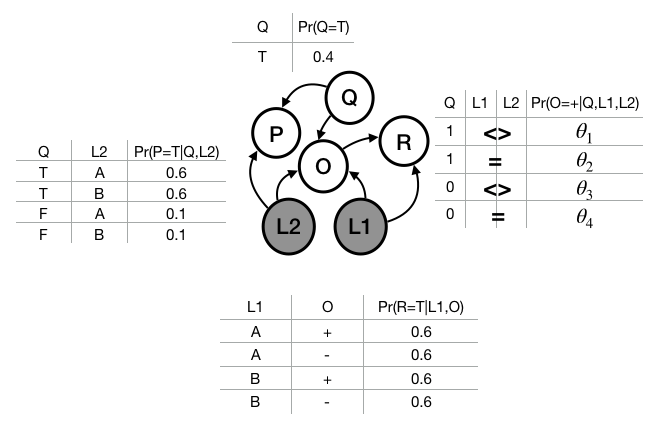
\includegraphics[width=\textwidth]{figs/BN.png}
  \end{minipage}\hfill
  \begin{minipage}[c]{0.45\textwidth}
    \caption{
        \small The model used for generating the datasets. There are four binary random variables, P, Q, O, and R. \textbf{P}: indicates whether or not the employee has high performance; \textbf{Q}: indicates whether or not an employee has high qualification; \textbf{O}: indicates whether or not the colleague submits the positive opinion towards the employee;  \textbf{R}: indicates whether or not the colleague has a positive opinion towards the employee;  \textbf{L1, L2}: indicates the label of the review provider and review receiver (observed).
    } \label{fig:BN}
  \end{minipage}
\end{figure}

We show the effectiveness of FairPSL by performing an empirical evaluation. We investigate two research questions in our experiments:
\begin{description}
\item[Q1] What is the effect of the fairness threshold $\delta$ on the fairness measures $RD/RC/RR$?
\item[Q2] How is decision quality affected by imposing $\delta$-fairness constraints?
\end{description}

Note that although we present the result for specific parameters of the framework in this section, we ran extensive analysis and the results we present are representative. We implemented the MAP inference routines of PSL and FairPSL in Python, using Gurobi-8.1\footnote{\url{www.gurobi.com}} as the backend solver. The FairPSL code, code for the data generator and data is publicly available\footnote{https://github.com/gfarnadi/FairPSL}. 

\subsection{Data generation}
  
We evaluate the FairPSL inference algorithm on synthetic datasets representing the performance review scenario (introduced in Example~\ref{ex:review}). The organization hierarchy is generated synthetically. 
The organization hierarchy generator is parameterized by two numbers: the number of employees in the organization ($n$) and the number of employees managed by each manager ($k$). Each employee is randomly assigned with a label \emph{A} or \emph{B}. An examples organization hierarchy with $n$=50 and $k$=3 is shown in Figure~\ref{fig:hierachy}.

\begin{figure}
  \begin{minipage}[c]{0.3\textwidth}
    \caption{
        \small An example of an organizational hierarchy with five levels and 50 employees with k=3. Each employee either has label A (shown with grey) or B (shown with white).
    }\label{fig:hierachy} 
	\end{minipage} \hfill
    \begin{minipage}[c]{0.7\textwidth}
    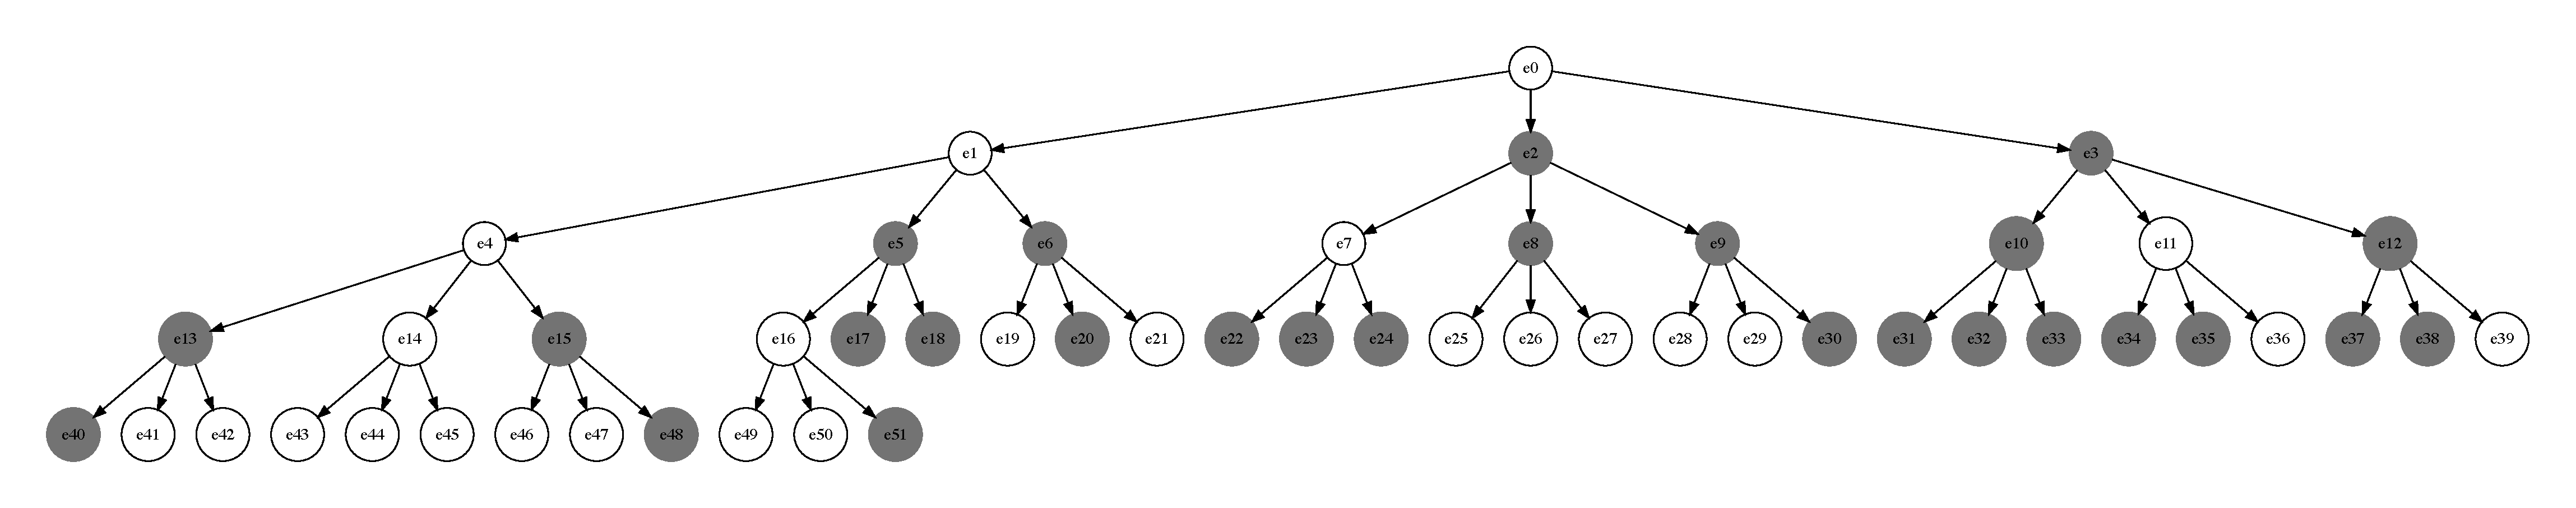
\includegraphics[width=\textwidth]{figs/Uni-hierachy.pdf}
  \end{minipage}
\end{figure}

For each employee, we use the generative model of Figure~\ref{fig:BN} to draw assignments for all the random variables. We assume that only $40\%$ of employees are qualified for promotion and regardless of their labels, employees submit only $60\%$ of their opinions. In addition, due to various personal and environmental factors, only $60\%$ of high quality employees perform well while $10\%$ of low quality employees also perform well regardless of their labels. Note that these numbers are not specific and just chosen for the framework to serve as a representative setting and a proof of concept. The conditional probability table for the opinion variable $O$ is parameterized by four values $(\theta_1, \theta_2, \theta_3, \theta_4)$ which together determine the degree of discrimination against the protected group. Since other parameters in the Bayesian network did not have a direct effect on the degree of discrimination, we fixed them to arbitrary values. 

The results presented in this section are based on an organization hierarchy  with $100$ employees where $k=5$. However, the results of the framework are not sensitive to the settings as we test the framework with various organization sizes ranging from $50$ to $500$ employees and various degree for $k$ ranging from $3$ to $10$. We generated seven datasets given the organization hierarchy using different values for the $\theta$ parameters: $(0.0,1.0,0.0,0.0)$, $(0.33,1.0,0.0,0.0)$, $(0.66,1.0,0.0,0.0)$, $(1.0,1.0,0.0,0.0)$, $(1.0,1.0,0.0,0.33)$, $(1.0,1.0,0.0,0.66)$, $(1.0,1.0,0.0,1.0)$. 
 
In the first three settings the discrimination originates from negative opinions towards qualified outgroup employees. The first setup is an extreme case where the opinion towards outgroup employees is always negative. The discrimination in the last three settings originates from positive opinions towards unqualified ingroup employees. The last setup is an extreme case where the opinion towards ingroup employees is always positive. The fourth setup represent unbiased opinions where employees are treated similarly based on their qualification. 

\paragraph{MAP Inference} We use the model presented in Table~\ref{tab:pslmodel} for MAP inference in PSL and FairPSL (recall that in FairPSL, the $\delta$-fairness constraints corresponding to one of the fairness measures are also added to the model). The observed atoms are $\textit{Manager(m,e)}$, $\textit{PositiveReview(e1,e2)}$ and labels of all employees. The truth values for all other atoms are obtained via MAP inference. We use the truth values obtained for the decision atoms $\textit{ToPromote(e)}$ to compute the fairness measures. We defined the discriminative pattern, and the protected and unprotected groups of this problem in Section~\ref{sec:formulation}.


\subsection{Evaluation results}

\begin{figure}
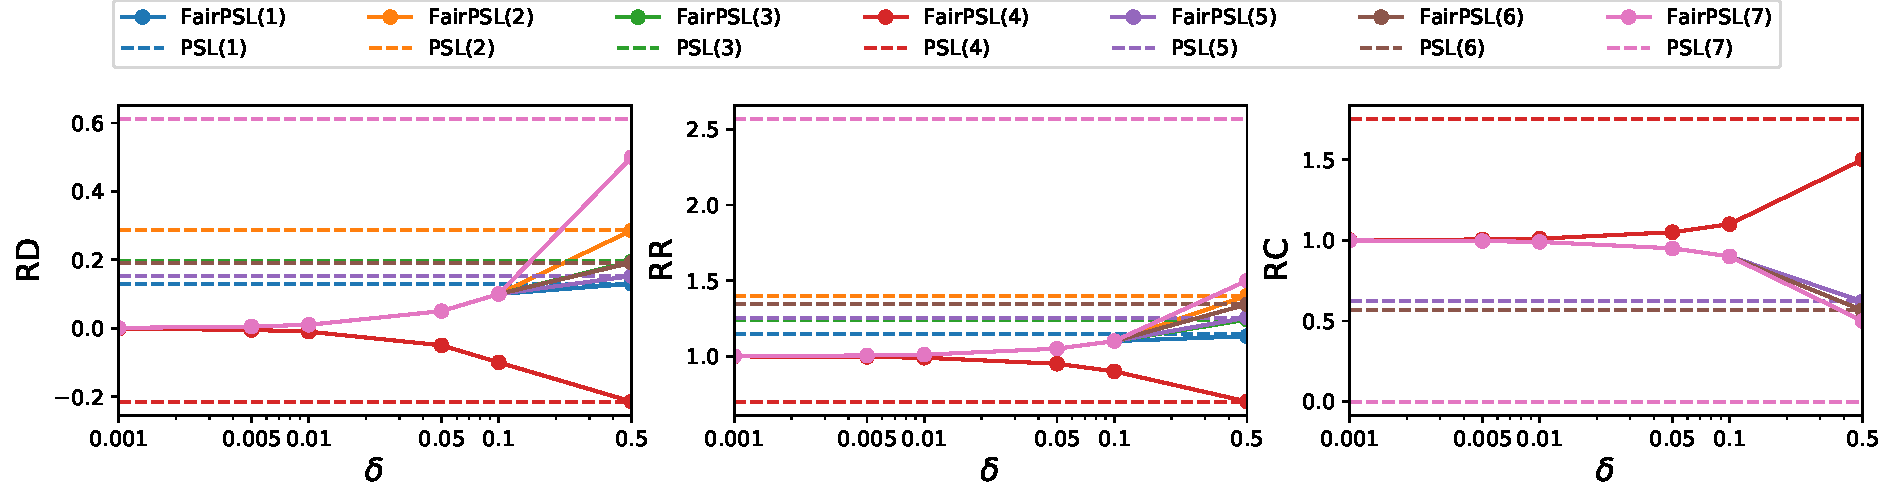
\includegraphics[width=1\linewidth]{figs/results_vis_uni_params.pdf}
\caption{\small Fairness score of predictions obtained by MAP inference of PSL and FairPSL, according to the fairness measures \emph{RD}, \emph{RR}, and \emph{RC}. The labels of datasets are mentioned with parenthesis next to the inference method. The FairPSL values of each measure are obtained by adding the $\delta$-fairness constraint of that measure.\label{fig:results}
}  
\end{figure}

To answer \textbf{Q1}, we run the MAP inference algorithm of PSL and FairPSL on seven synthetic datasets. 
We run the MAP inference of FairPSL multiple times on each dataset: For each of the three fairness measures, we add the corresponding $\delta$-fairness constraint with five thresholds $\{0.001, 0.005, 0.01, 0.05, 0.1, 0.5\}$.

Figure~\ref{fig:results} shows the fairness score of predictions in terms of the three fairness measures. As expected, tighter $\delta$-fairness constraints lead to better scores. Note that the best possible score according to RD is 0, as it computes a difference. Since RR and RC compute ratios, the best possible score according to these measures is 1. In our experiments, with any of these measures, taking $\delta = 0.001$ pushes the score of predictions to its limit.  

The $\delta$-fairness constraints modify the optimization problem of MAP inference by reducing the feasible region to solutions that conform with fairness guarantees. Research question \textbf{Q2} is concerned with the effect of this reduction on the accuracy of predictions. Note that decision quality is the same as the accuracy of predictions. To answer this question, we compare the inferred values for the decision atoms \textit{ToPromote(e)} against their actual values. These values are extracted from the known values of \textit{IsQualified(e)} according to rules 11 and 12 in Table~\ref{tab:pslmodel}. Figure~\ref{fig:accuracy} shows the area under the curve of the receiver operating characteristic~(AUC) of predicting the decision variable in three groups, namely the protected group, the unprotected group (i.e., promotion of the employees who have in-group managers), and all employees. By doing so, we make sure that our fairness constraints do not propagate bias towards either of the populations. Since the results of FairPSL with $\delta$-fairness constraints RR and RC are very similar to the results of RD, we only report the latter here.


\begin{figure}
    \centering
    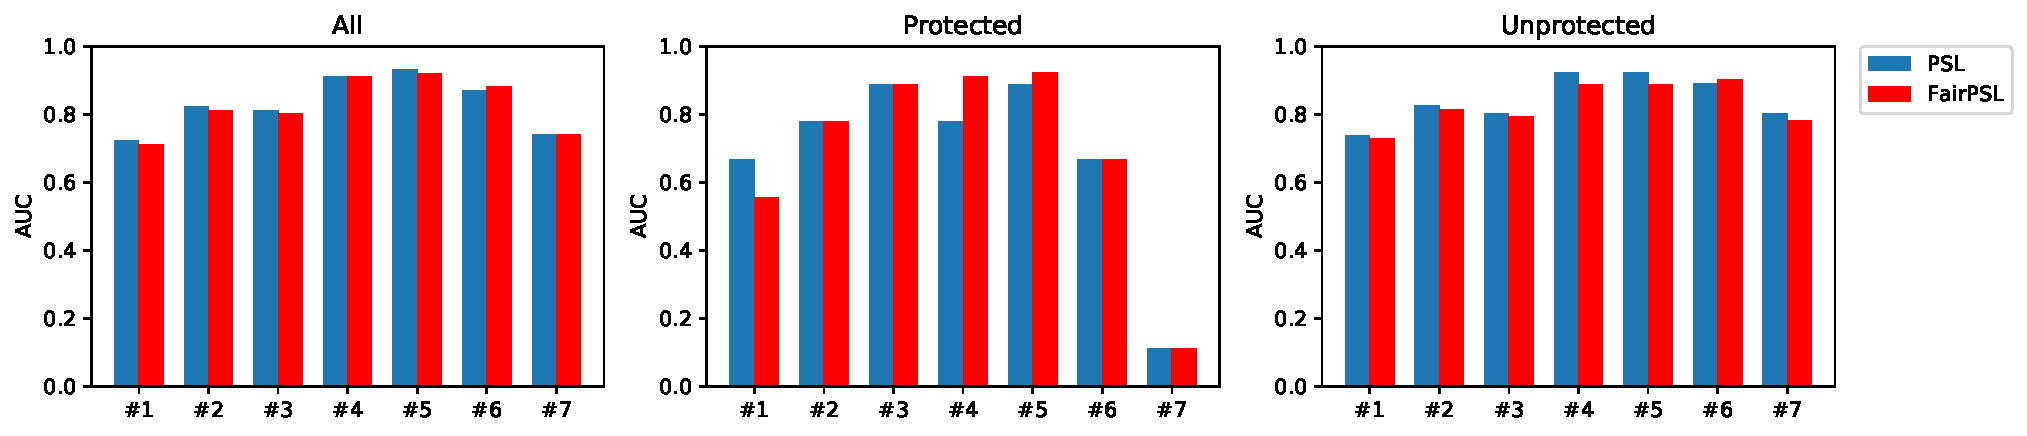
\includegraphics[width=\textwidth]{figs/roc.pdf}
    \caption{\small AUC score of predictions for truth values of unknown atoms \textit{ToPromote(e)} using MAP inference of PSL and FairPSL with $\delta$-fairness constraints $RD$ with $\delta=0.001$.}
    \label{fig:accuracy}
\end{figure}

According to Figure~\ref{fig:accuracy}, the results of both PSL and FairPSL in all seven datasets are close to each other. Note that although fairness may impose a cost in terms of overall accuracy, FairPSL often improves the accuracy of the protected class. Sometimes the overall predictions of FairPSL are even slightly better than PSL (e.g., dataset 6 and 7). As expected, the accuracy of the fourth setting where the opinions are unbiased are similar in both PSL and FairPSL. We observe that prediction of MAP inference for both FairPSL and PSL are similar, thus, in these settings at least, FairPSL guarantees fairness without hurting accuracy. Further investigation is required on the effect of the various ranges of discrimination (i.e., $\theta_1$, $\theta_2$, $\theta_3$, $\theta_4$) on the prediction results of FairPSL.



We also generate various types of organizations in which labels are not uniformly distributed, e.g., one population only occurs at the bottom levels of an organization. While we did not observe any differences in the behavior of our method with respect to accuracy and fairness measure, we found that the degree of discrimination is higher in such organizations. Further investigations on the structure of an organization on discrimination is an interesting direction for future research. 

\section{Conclusion and Future Directions}
\label{sec:conclusion}
Many applications of AI and machine learning affect peoples' lives in important ways. While there is a growing body of work on fairness in AI and ML, it assumes an individualistic notion of fairness.   In this paper, we have proposed a general framework for relational fairness which includes both a rich language for defining discrimination patterns and an efficient algorithm for performing inference subject to fairness constraints. We show our approach enforces fairness guarantees while preserving the accuracy of the predictions. 

There are many avenues for expanding on this work. For example, here we assumed that the discriminative pattern is given, however an automatic mechanism to extract discriminatory situations hidden in a large amount of decision records is an important and required task. Discrimination discovery has been studied for attribute-based fairness~\cite{pedreschi2013discovery}. An interesting next step is discrimination pattern discovery in relational data.

\section*{Acknowledgements}
This work is supported by the National Science Foundation under Grant Numbers CCF-1740850 and IIS-1703331. Golnoosh Farnadi and Behrouz Babaki are  supported by postdoctoral scholarships from IVADO through the Canada First Research Excellence Fund (CFREF) grant.

\begin{thebibliography}{10}
\itemsep=1pt 
\begin{small}

\bibitem{EUlaw}
European union legislation. (a) racial equality directive, 2000; (b) employment
  equality directive, 2000; (c) gender employment directive, 2006; (d) equal
  treatment directive (proposal), 2008.

\bibitem{UKlaw}
{UK} legislation. (a) sex discrimination act, 1975, (b) race relation act,
  1976.

\bibitem{USlaw}
United nations legislation. (a) universal declaration of human rights, 1948,
  (c) convention on the elimination of all forms of racial discrimination,
  1966, (d) convention on the elimination of all forms of discrimination
  against women, 1979.

\bibitem{alshukaili:iswc16}
Duhai Alshukaili, Alvaro A.~A. Fernandes, and Norman~W. Paton.
\newblock Structuring linked data search results using probabilistic soft
  logic.
\newblock In {\em International Semantic Web Conference {(1)}}, volume 9981 of
  {\em Lecture Notes in Computer Science}, pages 3--19, 2016.

\bibitem{bach:jmlr17}
Stephen~H. Bach, Matthias Broecheler, Bert Huang, and Lise Getoor.
\newblock Hinge-loss markov random fields and probabilistic soft logic.
\newblock {\em Journal of Machine Learning Research}, 18:109:1--109:67, 2017.

\bibitem{barocas2016big2}
Solon Barocas and Andrew~D Selbst.
\newblock Big data's disparate impact.
\newblock {\em California Law Review}, 104:671, 2016.

\bibitem{boyd2014networked}
Danah Boyd, Karen Levy, and Alice Marwick.
\newblock The networked nature of algorithmic discrimination.
\newblock In {\em Data and discrimination: Collected essays}, pages 53--57.
  2014.

\bibitem{brewer1979group}
Marilynn~B Brewer.
\newblock In-group bias in the minimal intergroup situation: A
  cognitive-motivational analysis.
\newblock {\em Psychological bulletin}, 86(2):307, 1979.

\bibitem{brewer2007social}
Marilynn~B Brewer.
\newblock The social psychology of intergroup relations: Social categorization,
  ingroup bias, and outgroup prejudice.
\newblock {\em Social Psychology: Handbook of Basic Principles}, 2007.

\bibitem{chouldechova2017fair2}
Alexandra Chouldechova.
\newblock Fair prediction with disparate impact: {A} study of bias in
  recidivism prediction instruments.
\newblock {\em CoRR}, abs/1703.00056, 2017.

\bibitem{dwork2012fairness3}
Cynthia Dwork, Moritz Hardt, Toniann Pitassi, Omer Reingold, and Richard~S.
  Zemel.
\newblock Fairness through awareness.
\newblock In {\em {ITCS}}, pages 214--226. {ACM}, 2012.

\bibitem{ebrahimi:emnlp16}
Javid Ebrahimi, Dejing Dou, and Daniel Lowd.
\newblock Weakly supervised tweet stance classification by relational
  bootstrapping.
\newblock In {\em {EMNLP}}, pages 1012--1017. The Association for Computational
  Linguistics, 2016.

\bibitem{farnadi2018fairness}
Golnoosh Farnadi, Behrouz Babaki, and Lise Getoor.
\newblock Fairness in relational domains.
\newblock In {\em AAAI/ACM Conference on AI, Ethics, and Society (AIES)}, pages
  108--114. ACM, 2018.

\bibitem{feldman2015certifying2}
Michael Feldman, Sorelle~A. Friedler, John Moeller, Carlos Scheidegger, and
  Suresh Venkatasubramanian.
\newblock Certifying and removing disparate impact.
\newblock In {\em {KDD}}, pages 259--268. {ACM}, 2015.

\bibitem{getoor2007introduction}
Lise Getoor and Ben Taskar.
\newblock {\em {Introduction to Statistical Relational Learning}}.
\newblock MIT press Cambridge, 2007.

\bibitem{hardt2016equality3}
Moritz Hardt, Eric Price, and Nati Srebro.
\newblock Equality of opportunity in supervised learning.
\newblock In {\em {NIPS}}, pages 3315--3323, 2016.

\bibitem{kamishima2011fairness}
Toshihiro Kamishima, Shotaro Akaho, and Jun Sakuma.
\newblock Fairness-aware learning through regularization approach.
\newblock In {\em ICDMW}, pages 643--650. {IEEE} Computer Society, 2011.

\bibitem{kouki:recsys15}
Pigi Kouki, Shobeir Fakhraei, James~R. Foulds, Magdalini Eirinaki, and Lise
  Getoor.
\newblock Hyper: {A} flexible and extensible probabilistic framework for hybrid
  recommender systems.
\newblock In {\em RecSys}, pages 99--106. {ACM}, 2015.

\bibitem{counterfactualfairness}
Matt~J. Kusner, Joshua~R. Loftus, Chris Russell, and Ricardo Silva.
\newblock Counterfactual fairness.
\newblock In {\em {NIPS}}, pages 4069--4079, 2017.

\bibitem{Pedreschi:2012}
Dino Pedreschi, Salvatore Ruggieri, and Franco Turini.
\newblock A study of top-k measures for discrimination discovery.
\newblock In {\em {SAC}}, pages 126--131. {ACM}, 2012.

\bibitem{pedreschi2013discovery}
Dino Pedreschi, Salvatore Ruggieri, and Franco Turini.
\newblock The discovery of discrimination.
\newblock In {\em Discrimination and Privacy in the Information Society},
  volume~3 of {\em Studies in Applied Philosophy, Epistemology and Rational
  Ethics}, pages 91--108. Springer, 2013.

\bibitem{ridgeway2004unpacking}
Cecilia~L Ridgeway and Shelley~J Correll.
\newblock Unpacking the gender system: A theoretical perspective on gender
  beliefs and social relations.
\newblock {\em Gender \& society}, 18(4):510--531, 2004.

\bibitem{sridhar:bioinformatics16}
Dhanya Sridhar, Shobeir Fakhraei, and Lise Getoor.
\newblock A probabilistic approach for collective similarity-based drug-drug
  interaction prediction.
\newblock {\em Bioinformatics}, 32(20):3175--3182, 2016.

\bibitem{verma2018fairness2}
Sahil Verma and Julia Rubin.
\newblock Fairness definitions explained.
\newblock In {\em 2018 IEEE/ACM International Workshop on Software Fairness
  (FairWare)}, pages 1--7. IEEE, 2018.

\bibitem{west2014exploiting}
Robert West, Hristo~S. Paskov, Jure Leskovec, and Christopher Potts.
\newblock Exploiting social network structure for person-to-person sentiment
  analysis.
\newblock {\em {TACL}}, 2:297--310, 2014.

\bibitem{zafar2017parity}
Muhammad~Bilal Zafar, Isabel Valera, Manuel Gomez{-}Rodriguez, Krishna~P.
  Gummadi, and Adrian Weller.
\newblock From parity to preference-based notions of fairness in
  classification.
\newblock In {\em {NIPS}}, pages 228--238, 2017.

\bibitem{zemel2013learning}
Richard~S. Zemel, Yu~Wu, Kevin Swersky, Toniann Pitassi, and Cynthia Dwork.
\newblock Learning fair representations.
\newblock In {\em {ICML} {(3)}}, volume~28 of {\em {JMLR} Workshop and
  Conference Proceedings}, pages 325--333. JMLR.org, 2013.

\end{small}
\end{thebibliography}

\end{document}

\end{article}



\begin{article}
{Learning Data Structure Alchemy}
{Stratos Idreos, 
Kostas Zoumpatianos, 
Subarna Chatterjee, 
Wilson Qin,
Abdul Wasay,
Brian Hentschel, 
Mike Kester,
Niv Dayan,
Demi Guo,
Minseo Kang,
Yiyou Sun
}
\graphicspath{{submissions/Learning/}}
%\documentclass[11pt,dvipdfm]{article}
\documentclass[11pt]{article}
\usepackage{deauthor,times,graphicx} %required
\usepackage{amsmath,amssymb}
\usepackage{multirow}
\usepackage{algorithm}
\usepackage{algpseudocode}
\usepackage{todonotes}
\usepackage{url}

% \graphicspath{{farnadi/}}

\newtheorem{mydef}{\textbf{Definition}}
\newtheorem{myex}{\textbf{Example}}
\newtheorem{mytheorem}{\textbf{Theorem}}


\begin{document}

\title{A Declarative Approach to Fairness in Relational Domains}
\author{Golnoosh Farnadi$^{1,2}$, Behrouz Babaki$^1$, Lise Getoor$^3$\\
$^1$Polytechnique Montr\'{e}al, $^2$ Mila, $^3$ UC Santa Cruz \\
farnadig@mila.quebec, behrouz.babaki@polymtl.ca, getoor@soe.ucsc.edu}

\maketitle

\begin{abstract}
AI and machine learning tools are being used with increasing frequency for decision making in domains that affect peoples' lives such as employment, education, policing and %loan approval
financial qualifications. These uses raise concerns about biases of algorithmic discrimination and have motivated the development of fairness-aware machine learning. However, existing fairness approaches are based solely on attributes of individuals. In many cases, discrimination is much more complex, and taking into account the social, organizational, and other connections between individuals is important. We introduce new notions of fairness that are able to capture the relational structure in a domain. We use first-order logic to provide a flexible and expressive language for specifying complex relational patterns of discrimination. Furthermore, we extend an existing statistical relational learning framework, probabilistic soft logic~(PSL), to incorporate our definition of relational fairness. We refer to this fairness-aware framework FairPSL. FairPSL makes use of the logical definitions of fairnesss but also supports a probabilistic interpretation. In particular, we show how to perform maximum a posteriori~(MAP) inference by exploiting probabilistic dependencies within the domain while avoiding violations of fairness guarantees. Preliminary empirical evaluation shows that we are able to make both accurate and fair decisions.
\end{abstract}

\section{Introduction}
\label{sec:introduction}

Over the past few years, AI and machine learning have become essential components in operations that drive the modern society, e.g., in financial, administrative, and educational spheres. \emph{Discrimination} happens when qualities of individuals which are not relevant to the decision making process influence the decision. Delegating decision making to an automated process raises questions about discriminating against individuals with certain traits based on biases in the data. This is especially important when the decisions have the potential to impact the lives of individuals, for example, the decisions on granting loans, assigning credit, and employment. 

\emph{Fairness} is defined as the absence of discrimination in a decision making process. The goal of \emph{fairness-aware} machine learning is to ensure that the decisions made by an algorithm do not discriminate against a population of individuals~\cite{feldman2015certifying2,boyd2014networked,hardt2016equality3}. Fairness has been well studied in the social sciences and legal scholarship (for an in-depth review see~\cite{barocas2016big2}), and there is emerging work on fairness-aware ML within the AI and computer science communities. For example, fairness through awareness/Lipschitz property~\cite{dwork2012fairness3}, individual fairness~\cite{zemel2013learning}, statistical parity/group fairness~\cite{kamishima2011fairness}, counterfactual fairness~\cite{counterfactualfairness}, demographic parity/disparate impact~\cite{feldman2015certifying2,chouldechova2017fair2}, preference-based fairness~\cite{zafar2017parity}, and equality of opportunity~\cite{hardt2016equality3}.

The existing work in fairness-aware machine learning is based on a definition of discrimination where a decision is influenced by an \emph{attribute} of an individual. An attribute value upon which discrimination is based (such as gender, race, or religion) is called a \emph{sensitive attribute}. The sensitive attribute defines a population of vulnerable individuals known as the \emph{protected group}. A fair decision-making process treats the protected group the same as the \emph{unprotected group}. 

However, in many social contexts, discrimination is the result of complex interactions and can not be described solely in terms of attributes of an individual. For example, consider an imaginary scenario in an organization in which younger female workers who have older male supervisors have lower chances of promotion than their male counterparts.\footnote{Of course, many other patterns may be possible: female bosses may promote female subordinates and discriminate against male workers, or male bosses may promote female employees.  Our goal is to provide a general framework which is able to describe arbitrarily complex discrimination patterns.} 
 This discrimination pattern involves two attributes of the individual (gender and age), a relationship with another individual (supervisor), and two attributes of the second individual. Addressing such complex cases poses two challenges. First, the concepts of discrimination and fairness need to be extended to capture not only attributes of individuals but also the relationships between them. Second, a process is required that ensures that fair decisions are made about individuals who are affected by such patterns. In this paper we address both of these challenges.
We use first-order logic (FOL) to extend the notion of fairness to the relational setting. FOL is an expressive representation for relational problems which is also widely used for learning in relational domains. Moreover, we extend an existing framework for statistical relational learning~\cite{getoor2007introduction} called probabilistic soft logic (PSL)\footnote{http://psl.linqs.org/}~\cite{bach:jmlr17}. PSL combines logic and probability for learning and reasoning over uncertain relational domains. One of the most common reasoning tasks in PSL is called maximum a posteriori (MAP) inference, which is performed by finding the most probable truth values for unknowns over a set of given evidence. We develop a new MAP inference algorithm which is able to maximize the a posteriori values of unknown variables \emph{subject to} fairness guarantees. An early version of this paper which this work builds upon and extends appeared in~\cite{farnadi2018fairness}.

\looseness-1
Our contributions are as follows: 1) we propose fairness-aware machine learning for the relational setting; 2) we extend PSL into a fairness-aware framework called FairPSL which can represent the logical definition of fairness; 3) we develop a new MAP inference algorithm which is able to maximize the posteriori values of unknown variables \emph{subject to} fairness guarantees; 4) we empirically evaluate our proposed framework on synthetic data. 

\section{Motivation}
\label{sec:motivation}

Discrimination in social contexts have been studied in the field of social psychology~\cite{brewer2007social,brewer1979group,ridgeway2004unpacking}. There is a large literature on various aspects of relational bias in social contexts such as \emph{in-group-out-group bias}, \emph{gender bias}, and \emph{ethnicity-based favoritism} that can result in discrimination. 
As an example, consider gender bias in the workplace that reflects stereotypically masculine criteria and male-based favoritism. Such gender bias 
typically places women in lower positions and negatively impacts their opportunities. Further, lack of women in leadership positions may affect the promotion of women and results in a glass ceiling that keeps women from rising beyond a certain level in the hierarchy. This scenario shows that considering  protected attributes such as gender is not always sufficient to detect the source of bias and avoid discrimination, one also has to consider the relational information, in this case the organization hierarchy. Note that this can be generalized to any ingroup/outgroup scenario where the sensitive attribute could be race, religion, age, marital-status, etc.

The existing work on designing fair algorithms in machine learning exclusively focuses on \emph{attribute-based fairness}, which is based on the following assumptions: First, there is an assumption that the individuals (sometimes referred to as units or entities) are independent and described by simple attribute vectors. Second, the group for which one wishes to ensure fairness (known as the \emph{protected group}) is defined on the basis of some attribute values. Finally, there is a decision that is associated with each individual, and the goal is to ensure that members of the protected group are subject to a fair decision (we discuss different fairness measures in Section~\ref{sec:fairnessmeasure}).  We illustrate  attribute-based fairness in the following example. 

\begin{myex}[Loan Processing]
\label{ex:loan}
A bank bases its decisions about granting a loan on attributes of the applicant. The goal is to decide whether to grant a loan to an applicant using a predictive model. The bank needs to ensure that the obey fair lending practices and ensure that gender, race, sexual orientation of applicants has no influence on the decision. In this scenario, the protected group is the historically disadvantaged applicants.  
\end{myex}
The current fairness-aware machine learning techniques are not capable of modeling relations and hence cannot be used to make the decision making model fair. However, in many decision making scenarios, especially in social and organizational settings, the domain is relational, and the protected group itself might be best represented using a relational definition. We illustrate this setting in the following scenario:
\begin{myex}[Performance Review]
\label{ex:review}
Consider an organization where decisions about the promotion of employees is based on two criteria: 1) an objective performance measure, and 2) the opinion of their direct and indirect managers above them. The opinions are inferred from the performance reviews which are collected periodically. Not every manager can submit a review for all its subordinates, this is especially the case for top-level managers who have a large number of subordinates. Hence, the opinions of managers are collectively inferred from the opinions of their sub-ordinates. However, some employees may be biased, and judge other employees unfavorably, by favoring employees who are similar to themselves (same gender, race, religion, etc.) over employees who are dissimilar. The organization needs to ensure that promotion of employees do not have any relational bias caused by in-group-out-group favoritism.

\end{myex}
Example~\ref{ex:review} describes a prediction problem over a database that consists of relations between employees. Such prediction tasks are best handled by techniques from the relational learning domain. To ensure fair prediction in such settings, we need to extend the notion of \emph{attribute-based fairness} to \emph{relational fairness}. Throughout this paper, we use the performance review problem as a running example for relational fairness.

\section{Fairness Formalism}
\label{sec:formulation}

A representation that can describe different types of entities and different relationships between them is called relational. In this section, we use first-order logic to define relational fairness. We employ first-order logic as an expressive representation formalism which can represent objects and complex relationships between them. We start by defining an atom:

\begin{mydef}[Atom]
An atom is an expression of the form $P(a_1, a_2, \ldots, a_n)$ where each argument $a_1, a_2,$ $\ldots,$ $a_n$ is either a constant or a variable. The finite set of all possible substitutions of a variable to a constant for a particular variable $a$ is called its \textit{domain} $D_{a}$. If all variables in $P(a_1, a_2, \ldots, a_n)$ are substituted by some constant from their respective domain, then we call the resulting atom a \textit{ground atom}. 
\end{mydef}

\begin{myex}
In our loan processing problem (Example~\ref{ex:loan}), we can represent applicants' attributes by atoms. For instance, atom $Female(v)$ indicates whether or not applicant $v$ is female. Similarly, we can represent relations with atoms. In the performance review problem in Example~\ref{ex:review} the atom $Manager(m,e)$ indicates whether or not employee $m$ is a direct or indirect manager of employee $e$.
\end{myex}

The relational setting provides the flexibility to express complex definitions with formulae.

\begin{mydef}[Formula] 
A formula is defined by induction: every atom is a formula. If $\alpha$ and $\beta$ are formulae, then $\alpha \vee \beta$, $\alpha \wedge \beta$, $\neg \alpha$, $\alpha \rightarrow \beta$ are formulae. If $x$ is a variable and $\alpha$ is a formula, then the quantified expressions of the form $\exists x$ $\alpha$ and $\forall x$ $\alpha$ are formulae.    
\end{mydef}

To characterize groups of individuals based on a formula, we define the notion of \emph{population}.

\begin{mydef}[Population]
We denote formula $F$ which has only one free variable $v$ (i.e., other variables in $F$ are quantified) by $F[v]$. The population defined by $F[v]$ is the set of substitutions of $v$ for which $F[v]$ holds.   
\end{mydef}


\begin{myex}
\label{ex:disformula}
Consider the formula $F[v] := \forall u, \, \textit{Manager}(u,v) \rightarrow \neg \textit{SameGroup}(u, v)$. The population specified by this formula is the set of individuals all of whose managers belong to a group different from theirs. 
\end{myex}

The truth value of a formula is derived from the truth value of atoms that it comprises, according to the rules of logic. Each possible assignment of truth values to ground atoms is called an \emph{interpretation}. 


\begin{mydef}[Interpretation]
An interpretation $I$ is a mapping that associates a truth value $I(P)$ to each ground atom $P$. For Boolean truth values, $I$ associates true to 1 and false to 0 truth values. For soft logic (see Definition~\ref{def:softlogic}) $I$ maps each ground atom $P$ to a truth value in interval $[0, 1]$.
\end{mydef}

In attribute-based fairness, it is assumed that there is a certain attribute of individuals, i.e, the sensitive attribute,  that we do not want to affect a decision. Gender, race, religion and marital status are examples of sensitive attributes. Discrimination has been defined in social science studies as a treatment in favor or against a group of individuals given their sensitive attribute. This group of individuals is the protected group. 

In a relational setting, both the sensitive attributes of an individual and their participation in various relations may have an undesired effect on the final decision. We characterize the protected group in a relational setting by means of a population. In practice, we are often interested in maintaining fairness for a specific population such as applicants, students, employees, etc. This population is then partitioned into the protected and unprotected groups. We define a \emph{discriminative pattern} which is a pair of formulae to capture these groups: 1) $F_1[v]$: to specify the difference between the protected and unprotected groups and 2) $F_2[v]$: to specify the population over which we want to maintain fairness. 

\begin{mydef}[Discriminative pattern]
A discriminative pattern is a pair $\textit{DP}[v]:=(F_1[v], F_2[v])$ , where $F_1[v]$ and $F_2[v]$ are formulae.
\end{mydef}

\begin{myex}
\label{ex:pattern}
The two formulae in the discrimination pattern $\textit{DP}[v]:= \big((\forall u, \,  \textit{Manager}(u,v) \rightarrow  \neg \textit{SameGroup}(u, v)),$ $\textit{Employee}(v)\big)$ specify two populations, namely all employees and those employees who belong to a group different from their managers.
\end{myex}

Given the definition of the discriminative pattern, we have a rich language to define the scope of the protected and unprotected groups in a relational setting.

\begin{mydef}[Protected group] Given an interpretation $I$, the protected group is a population of the form:
{$$PG :=\{ v : F_1[v] \wedge F_2[v]\}$$}
which is defined as the set of all instances hold for variable $v$ for which $F_1[v] \wedge F_2[v]$ is true under interpretation $I$, that is, $I(F_1[v] \wedge F_2[v]) = 1$. 
Similarly, the \emph{unprotected group} is a population of the form: 
{$$UG := \{ v : \neg F_1[v] \wedge  F_2[v]\}$$}
which is defined as the set of all instances hold for variable $v$ 
for which $I(\neg F_1[v] \wedge F_2[v]) = 1$. 
\end{mydef}

\begin{myex}
The protected group of the discrimination pattern specified in Example~\ref{ex:pattern} is {$PG := \big\{ v : \big(\forall u, \,$ $ \textit{Manager}(u, v) \rightarrow \neg \textit{SameGroup}(u, v)\big) \wedge \textit{Employee}(v) \big\}$} and the unprotected group is {$UG :=  \big\{ v:  \big(\exists u, \, \textit{Manager}(u,v) \wedge \textit{SameGroup}(u, v)\big) \wedge \textit{Employee}(v) \big\}$}. This means our protected group is the set of employees belonging to a group different from their managers,
and our unprotected group consists of other employees. 
\end{myex}

Discrimination is defined in terms of a treatment or decision that distinguishes between the protected and unprotected groups. Here we define the \emph{decision} atom.
\begin{mydef}[Decision atom] A decision atom $d(v)$ is an atom containing exactly one variable $v$ that specifies a decision affecting the protected group which is defined either by law or end-user.
\end{mydef}
\begin{myex}
The decision atom ${\textit ToPromote}(v)$ indicates whether or not $v$ receives a promotion.
\end{myex}

Note that the fairness formulation in this section is designed for the relational setting, however relational fairness subsumes the attribute-based fairness such that: a sensitive attribute is defined by an atom with one argument and $F_2[v]$ in discrimination pattern is $\textit{Applicant}(v)$. For example, discrimination pattern of our loan processing problem in Example~\ref{ex:loan} is of the form $\textit{DP} := ( \textit{Female}(v), \textit{Applicant}(v))$ that denotes female applicants as the protected group (i.e., $PG :=  \{ v: \textit{Female}(v) \}$) and male applicants as the unprotected group (i.e., $UG := \{ v: \neg \textit{Female}(v)\}$).


\section{Fairness Measures}
\label{sec:fairnessmeasure}

Over the past few years, many fairness measures have been introduced~\cite{verma2018fairness2}. An important class of these measures are \emph{group fairness} measures which quantify the inequality between different subgroups. Some of the most popular measures in this class include \emph{equal opportunity}, \emph{equalized odds}, and \emph{demographic parity}~\cite{hardt2016equality3}. In this paper we restrict our focus to the latter. In an attribute-value setting, demographic parity means that the decision should be independent of the protected attributes. Assume that binary variables $A$ and $C$ denote the decision and protected attributes, and the preferred value of $A$ is one. Demographic parity requires that:

\begin{equation*}
    P(A=1 | C=0) = P(A=1 | C=1)
\end{equation*}

We will now generalize this measure to the relational setting using the notations defined in Section~\ref{sec:formulation}. Let $a$ and $c$ denote the counts of denial (i.e., negative decisions) for protected and unprotected groups, and $n_{1}$ and $n_{2}$ denote their sizes, respectively. Given the decision atom $d(v)$, discriminative pattern $\textit{DP}(F_1[v], F_2[v])$, and interpretation $I$, these counts are computed by the following equations: 
{
\begin{flalign}
    & a \equiv \sum_{v \in D_v} I\big( \neg d(v) \wedge  F_1[v] \wedge F_2[v]) \label{eq:a}\\
    & c \equiv \sum_{v \in D_v} I\big( \neg d(v) \wedge  \neg F_1[v] \wedge  F_2[v]) \label{eq:c}\\
    & n_{1} \equiv \sum_{v \in D_v} I\big(F_1[v] \wedge F_2[v]) \label{eq:n1}\\
    & n_{2} \equiv \sum_{v \in D_v} I\big(\neg F_1[v] \wedge  F_2[v]) \label{eq:n2}
\end{flalign}}
The proportions of denying for protected and unprotected groups are $p_1 = \frac{a}{n_1}$ and $p_2 = \frac{c}{n_2}$, respectively. There are a number of data-driven measures~\cite{Pedreschi:2012} which quantify demographic disparity and can be defined in terms of $p_1$ and $p_2$:
\begin{itemize}
    \item \textbf{Risk difference}: $RD = p_1 - p_2$, also known as absolute risk reduction. 
    \item \textbf{Risk Ratio}: $RR = \frac{p_1}{p_2}$, also known as relative risk. 
    \item \textbf{Relative Chance}: $RC = \frac{1 - p_1}{1 - p_2}$ also, known as selection rate.
\end{itemize}
These measures have been used in the legal systems of European Union, UK, and US~\cite{EUlaw,UKlaw,USlaw}. Notice that RR is the ratio of the proportion of benefit denial between the protected and unprotected groups, while RC is the ratio of the proportion of benefit granted. Finally, we introduce the notion of $\delta$-fairness.

\begin{mydef}[$\delta$-fairness]
If a fairness measure for a decision making process falls within some $\delta$-window, then the process is \emph{$\delta\text{-fair}$}. Given $0 \leq \delta \leq 1$, the  $\delta$-windows for measures RD/RR/RC are defined as:
{\begin{flalign*}
	     - \delta \leq &RD \leq \delta \\
	     1- \delta \leq &RR \leq 1+ \delta\\
	     1- \delta \leq &RC \leq 1+ \delta
	\end{flalign*}}
\end{mydef}

To overcome the limitations of attribute-based fairness, we introduce a new statistical relational learning~(SRL) framework~\cite{getoor2007introduction} suitable for modelling fairness in relational domain. In the next section, we review probabilistic soft logic~(PSL). We then extend PSL with the definition of relational fairness introduced above in Section~\ref{sec:fairMAP}. Our fairness-aware framework, ``FairPSL'', is the first SRL framework that performs fair inference. 

\section{Background: Probabilistic Soft Logic}
\label{sec:psl}

In this section, we review the syntax and semantics of PSL, and in the next section we extend MAP inference in PSL with fairness constraints to define MAP inference in FairPSL.

PSL is a probabilistic programming language for defining hinge-loss Markov random fields~\cite{bach:jmlr17}. Unlike other SRL frameworks whose atoms are Boolean, atoms in PSL can take continuous values in the interval $[0,1]$. PSL is an expressive modeling language that can incorporate domain knowledge with first-order logical rules and has been used successfully in various domains, including bioinformatics~\cite{sridhar:bioinformatics16}, recommender systems~\cite{kouki:recsys15}, natural language processing~\cite{ebrahimi:emnlp16}, information retrieval~\cite{alshukaili:iswc16}, and social network analysis~\cite{west2014exploiting}, among many others. 
 
A PSL model is defined by a set of first-order logical rules called \emph{PSL rules}.

\begin{mydef} [PSL rule] a PSL rule $r$ is an expression of the form:
{\begin{equation}
\lambda_{r}: T_1 \land T_2 \land \ldots \land T_w \rightarrow H_1 \vee H_2 \vee \ldots \vee H_l
\end{equation}}

where { $T_1, T_2, \ldots, T_w, H_1, H_2, \ldots, H_l$} are atoms or negated atoms and { $\lambda_{r} \in \mathbb{R}^{+} \cup \infty$} is the weight of the rule $r$.  We call { $T_1 \land T_2 \land \ldots \land T_w$} the body of $r$ ($r_{body}$), and { $H_1 \vee H_2 \vee \ldots \vee H_l$} the head of $r$ ($r_{head}$).
\end{mydef}


Since atoms in PSL take on continuous values in the unit interval $[0,1]$, next we define soft logic to calculate the value of the PSL rules under an interpretation $I$.

\begin{mydef}[Soft logic]
\label{def:softlogic}
The ({$\tilde{\wedge}$}) and ({$\tilde{\vee}$}) and negation ({$\tilde{\neg}$}) are defined as follows. For {$m, n \in [0,1]$} we have: {$m \tilde{\wedge} n = \max(m+n -1, 0)$}, {$m \tilde{\vee} n = \min(m+n , 1)$} and {$\tilde{\neg} m = 1 - m$}. The $\, \tilde{} \,$ indicates the relaxation over Boolean values.
\end{mydef}

The probability of truth value assignments in PSL is determined by the rules' \emph{distance to satisfaction}.

\begin{mydef}[The distance to satisfaction]
The distance to satisfaction $d_{r}(I)$ of a rule $r$ under an interpretation $I$ is defined as:
{
\begin{equation}
d_{r}(I) = \max\{0, I(r_{body})-I(r_{head})\}
\end{equation}}
\end{mydef}

By using Definition~\ref{def:softlogic}, one can show that the closer the interpretation of a grounded rule $r$ is to 1, the smaller its distance to satisfaction. A PSL model induces a distribution over interpretations $I$. Let $R$ be the set of all grounded rules, then the probability density function is:
{
\begin{equation}
f(I) ={\frac{1}{Z}} \exp[-\sum_{r\in R} \lambda_{r}(d_{r}(I))^p]
\label{eq:potential}
\end{equation}
}
\noindent where { $\lambda_{r}$} is the weight of rule $r$, {
$Z = \int_{I} \exp[ -\sum_{r\in R} \lambda_{r}(d_{r}(I))^p]$
} is a normalization constant, and { $p \in \{1,2\}$} provides a choice of two different loss functions, $p=1$ (i.e., linear), and $p=2$ (i.e, quadratic). These probabilistic models are instances of hinge-loss Markov random fields~(HL-MRF)~\cite{bach:jmlr17}. The goal of maximum a posteriori (MAP) inference is to find the most probable truth assignments $I_{\textit{MPE}}$ of unknown ground atoms given the evidence which is defined by the interpretation $I$. Let $X$ be all the evidence, i.e., $X$ is the set of ground atoms such that $\forall x \in X, I(x)$ is known, and let $Y$ be the set of ground atoms such that $\forall y \in Y, I(y)$ is unknown. Then we have
{
\begin{equation}
I_{\textit{MAP}}(Y) = \textit{arg}\max_{I(Y)} P(I(Y)|I(X))
\end{equation}}
Maximizing the density function in Equation~\ref{eq:potential} is equivalent to minimizing the weighted sum of the distances to satisfaction of all rules in PSL. 

\begin{table*}[t]
    \centering
    \begin{tabular}{|lll|}
    \hline
    &&\\
    $R1$ & $\lambda_1$ &: $\textit{IsQualified}(e) \rightarrow \textit{HighPerformance}(e)$ \\
    $R2$ & $\lambda_1$ &: $\neg \textit{IsQualified}(e) \rightarrow \neg \textit{HighPerformance}(e)$ \\
    $R3$ & $\infty$ &: $\textit{PositiveReview}(e1, e2) \rightarrow \textit{PositiveOpinion}(e1, e2)$ \\
    $R4$ & $\infty$ &: $\neg \textit{PositiveReview}(e1, e2) \rightarrow \neg \textit{PositiveOpinion}(e1, e2)$ \\
    $R5$ & $\lambda_1$ &: $\textit{PositiveOpinion}(e1, e2) \wedge \textit{Manager}(m, e1) \rightarrow \textit{PositiveOpinion}(m, e2)$ \\
    $R6$ & $\lambda_1$ &: $\neg \textit{PositiveOpinion}(e1, e2) \wedge \textit{Manager}(m, e1) \rightarrow \neg \textit{PositiveOpinion}(m, e2)$ \\
    $R7$ & $\lambda_1$ &: $\textit{PositiveOpinion}(m, e) \wedge \textit{Manager}(m, e) \rightarrow \textit{IsQualified}(e)$ \\
    $R8$ & $\lambda_1$ &: $\neg \textit{PositiveOpinion}(m, e) \wedge \textit{Manager}(m, e) \rightarrow \neg \textit{IsQualified}(e)$ \\
    $R9$ &  $\lambda_1$ &: $\neg \textit{ToPromote}(e)$\\
    $R10$ & $\infty$ &: $\textit{IsQualified}(e) \rightarrow \textit{ToPromote}(e)$ \\
    $R11$ & $\infty$ &: $\neg \textit{IsQualified}(e) \rightarrow \neg \textit{ToPromote}(e)$ \\
    &&\\
    \hline
    \end{tabular}
    \caption{\small A simplified PSL model for the \emph{Performance Reviewing} problem}
    \label{tab:pslmodel}
\end{table*}

\begin{myex}
\label{ex:pslmodel}
The simplified PSL model for the performance reviewing problem in Example\ref{ex:review} is given in Table~\ref{tab:pslmodel}. The goal of MAP inference for this problem is to infer employees to promote. We simplified the model by assigning the same weight to all soft rules (i.e., $\lambda_i= 1$ where $i=\{1,2,5,6,7,8,9\}$). Below we explain the meaning of each rule in the model.

Rule $R1$ indicates that qualified employees have high performance and similarly rule $R2$ expresses that a negative qualification of employees is derived from their low performance. Rules $R5$ and $R6$ presents the propagation of opinion from bottom to top of the organizational hierarchy, i.e., managers have similar opinions towards employees given the opinions of their sub-ordinate managers. And rules $R7$ and $R8$ indicate that the positive/negative opinion of direct/indirect managers derive from the qualification of an employee. Rule $R9$ indicates the prior that not all employees get promoted. We also have four hard constraints (i.e., rules $R3$, $R4$, $R10$ and $R11$) where the weight of the rules are $\infty$. Rules $R3$ and $R4$ indicate that submitted positive/negative reviews should reflect positive/negative opinions. And two rules $R10$ and $R11$ show that a highly qualified employee should get promoted. 
\end{myex}

\section{Fairness-aware PSL (FairPSL)}
\label{sec:fairMAP}

The standard MAP inference in PSL aims at finding values that maximize the conditional probability of unknowns. Once a decision is made according to these values, one can use the fairness measure to quantify the degree of discrimination. A simple way to incorporate fairness in MAP inference is to add the $\delta$-fairness constraints to the corresponding optimization problem.   

Consider risk difference, $\textit{RD}$, where $\textit{RD} \equiv \frac{\mathbf{a}}{n_1} - \frac{\mathbf{c}}{n_2}$. The $\delta$-fairness constraint $-\delta \leq \textit{RD} \leq \delta$ can be encoded as the following constraints:
{\begin{align}
    & n_2 \mathbf{a} - n_1 \mathbf{c} - n_1 n_2 \delta \leq 0 \label{eq:RD1}\\
    & n_2 \mathbf{a} - n_1 \mathbf{c} + n_1 n_2 \delta \geq 0
\end{align}}
Similarly, from $\textit{RR} \equiv \frac{\mathbf{a} / n_1}{\mathbf{c} / n_2}$ and the $\delta$-fairness constraint $1 - \delta \leq \textit{RR} \leq 1 + \delta$ we obtain:
{\begin{align}
    & n_2 \mathbf{a} - (1 + \delta) n_1 \mathbf{c} \leq 0 \\
    & n_2 \mathbf{a} - (1 - \delta) n_1 \mathbf{c} \geq 0
\end{align}}
And finally, $\textit{RC} \equiv \frac{1 - \mathbf{a} / n_1}{1 - \mathbf{c} / n_2}$ and the $\delta$-fairness constraint $1 - \delta \leq \textit{RC} \leq 1 + \delta$ gives:
{ \begin{align}
    & - n_2 \mathbf{a} + (1 + \delta) n_1 \mathbf{c} - \delta n_1 n_2 \leq 0 \\
    & - n_2 \mathbf{a} + (1 - \delta) n_1 \mathbf{c} + \delta n_1 n_2 \geq 0 \label{eq:RC2}
\end{align}}
A primary advantage of PSL over similar frameworks is that its MAP inference task reduces to a convex optimization problem which can be solved in polynomial time. To preserve this advantage, we need to ensure that the problem will remain convex after the addition of $\delta$-fairness constraints. 

\begin{mytheorem}
The following condition is sufficient for preserving the convexity of MAP inference problem after addition of $\delta$-fairness constraints: The formulae $F_1[v]$ and $F_2[v]$ do not contain an atom $y \in Y$ and all atoms in $F_1[v]$ and $F_2[v]$ have values zero or one.
\end{mytheorem}
\begin{proof}
Since $I(F_1[v])$ and $I(F_2[v])$ do not depend on $I(Y)$, the values $n_{1}$ and $n_{2}$ are constants that can be computed in advance. Let us define the sets $D_v^a = \{ v \in D_v : F_1[v] \wedge F_2[v] \, \text{is true} \}$ and $D_v^c = \{ v \in D_v : \neg F_1[v] \wedge F_2[v] \, \text{is true} \}$. Since $F_1[v]$ and $F_2[v]$ can be only zero or one, we can rewrite the equations~\ref{eq:a} and \ref{eq:c} as:
{
\begin{align*}
    & \mathbf{a} = \sum_{v \in D_v^a} I(\neg d(v)) = |D_v^a| - \sum_{v \in D_v^a} I(d(v))\\
    & \mathbf{c} = \sum_{v \in D_v^c} I(\neg d(v)) = |D_v^c| - \sum_{v \in D_v^c} I(d(v))
\end{align*}}
\noindent which indicates that $\mathbf{a}$ and $\mathbf{c}$ can be expressed as linear combinations of variables in the optimization problem. This means that constraints~\ref{eq:RD1}-\ref{eq:RC2} are linear. Hence, addition of these constraints preserves the convexity of the optimization problem. 
\end{proof}

\section{Experiments}
\label{sec:experiment}

\begin{figure}
  \begin{minipage}[c]{0.6\textwidth}
    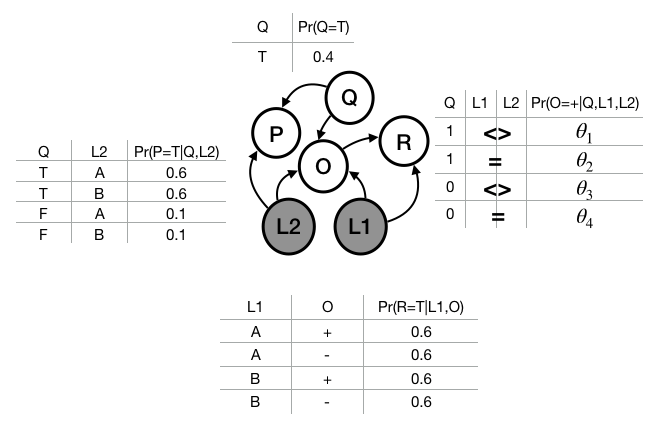
\includegraphics[width=\textwidth]{figs/BN.png}
  \end{minipage}\hfill
  \begin{minipage}[c]{0.45\textwidth}
    \caption{
        \small The model used for generating the datasets. There are four binary random variables, P, Q, O, and R. \textbf{P}: indicates whether or not the employee has high performance; \textbf{Q}: indicates whether or not an employee has high qualification; \textbf{O}: indicates whether or not the colleague submits the positive opinion towards the employee;  \textbf{R}: indicates whether or not the colleague has a positive opinion towards the employee;  \textbf{L1, L2}: indicates the label of the review provider and review receiver (observed).
    } \label{fig:BN}
  \end{minipage}
\end{figure}

We show the effectiveness of FairPSL by performing an empirical evaluation. We investigate two research questions in our experiments:
\begin{description}
\item[Q1] What is the effect of the fairness threshold $\delta$ on the fairness measures $RD/RC/RR$?
\item[Q2] How is decision quality affected by imposing $\delta$-fairness constraints?
\end{description}

Note that although we present the result for specific parameters of the framework in this section, we ran extensive analysis and the results we present are representative. We implemented the MAP inference routines of PSL and FairPSL in Python, using Gurobi-8.1\footnote{\url{www.gurobi.com}} as the backend solver. The FairPSL code, code for the data generator and data is publicly available\footnote{https://github.com/gfarnadi/FairPSL}. 

\subsection{Data generation}
  
We evaluate the FairPSL inference algorithm on synthetic datasets representing the performance review scenario (introduced in Example~\ref{ex:review}). The organization hierarchy is generated synthetically. 
The organization hierarchy generator is parameterized by two numbers: the number of employees in the organization ($n$) and the number of employees managed by each manager ($k$). Each employee is randomly assigned with a label \emph{A} or \emph{B}. An examples organization hierarchy with $n$=50 and $k$=3 is shown in Figure~\ref{fig:hierachy}.

\begin{figure}
  \begin{minipage}[c]{0.3\textwidth}
    \caption{
        \small An example of an organizational hierarchy with five levels and 50 employees with k=3. Each employee either has label A (shown with grey) or B (shown with white).
    }\label{fig:hierachy} 
	\end{minipage} \hfill
    \begin{minipage}[c]{0.7\textwidth}
    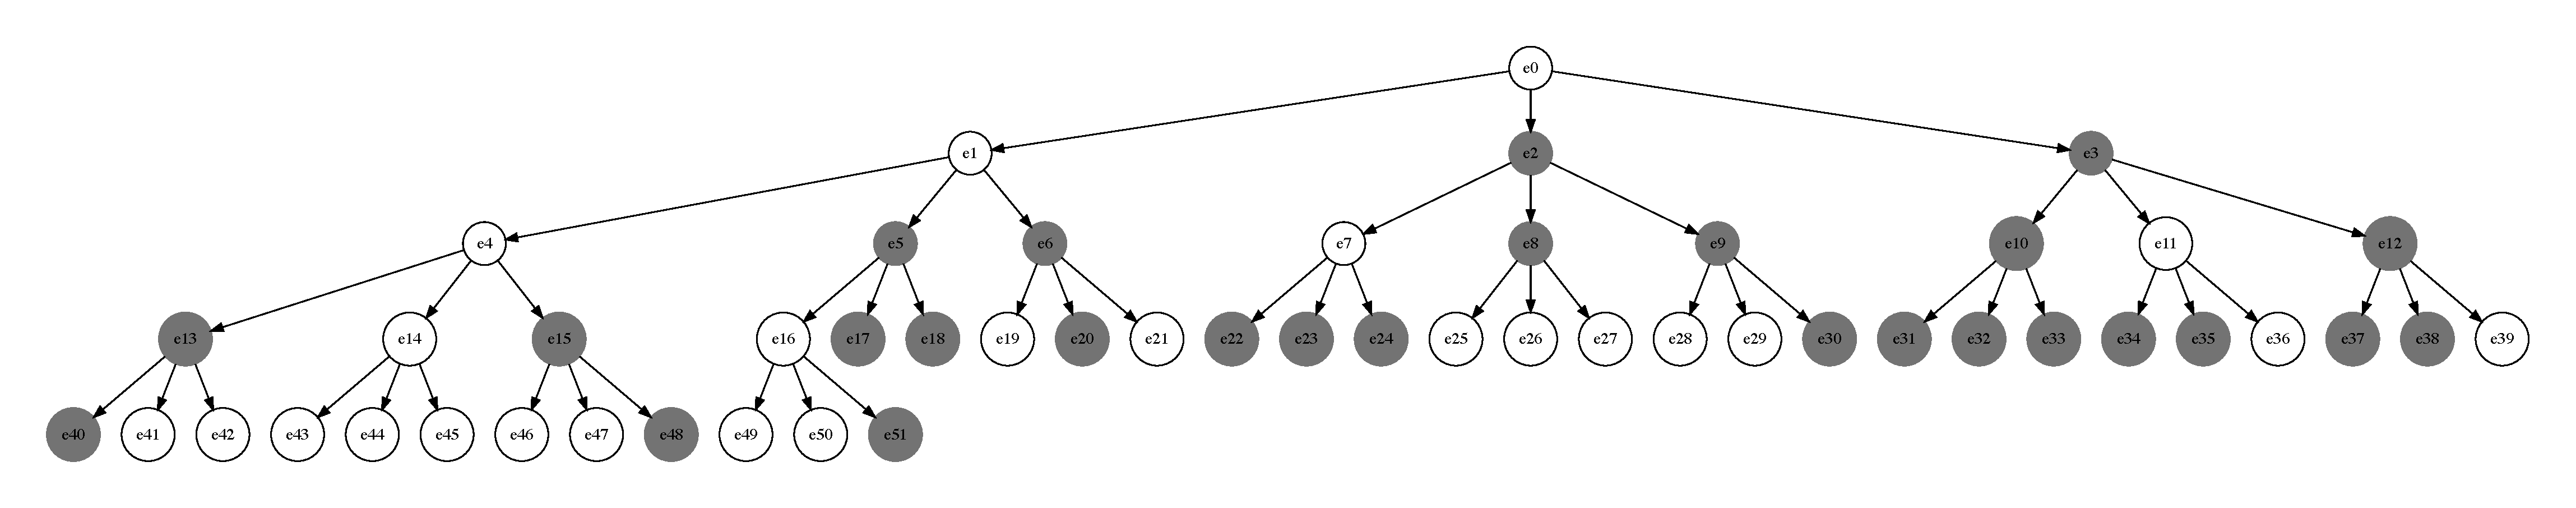
\includegraphics[width=\textwidth]{figs/Uni-hierachy.pdf}
  \end{minipage}
\end{figure}

For each employee, we use the generative model of Figure~\ref{fig:BN} to draw assignments for all the random variables. We assume that only $40\%$ of employees are qualified for promotion and regardless of their labels, employees submit only $60\%$ of their opinions. In addition, due to various personal and environmental factors, only $60\%$ of high quality employees perform well while $10\%$ of low quality employees also perform well regardless of their labels. Note that these numbers are not specific and just chosen for the framework to serve as a representative setting and a proof of concept. The conditional probability table for the opinion variable $O$ is parameterized by four values $(\theta_1, \theta_2, \theta_3, \theta_4)$ which together determine the degree of discrimination against the protected group. Since other parameters in the Bayesian network did not have a direct effect on the degree of discrimination, we fixed them to arbitrary values. 

The results presented in this section are based on an organization hierarchy  with $100$ employees where $k=5$. However, the results of the framework are not sensitive to the settings as we test the framework with various organization sizes ranging from $50$ to $500$ employees and various degree for $k$ ranging from $3$ to $10$. We generated seven datasets given the organization hierarchy using different values for the $\theta$ parameters: $(0.0,1.0,0.0,0.0)$, $(0.33,1.0,0.0,0.0)$, $(0.66,1.0,0.0,0.0)$, $(1.0,1.0,0.0,0.0)$, $(1.0,1.0,0.0,0.33)$, $(1.0,1.0,0.0,0.66)$, $(1.0,1.0,0.0,1.0)$. 
 
In the first three settings the discrimination originates from negative opinions towards qualified outgroup employees. The first setup is an extreme case where the opinion towards outgroup employees is always negative. The discrimination in the last three settings originates from positive opinions towards unqualified ingroup employees. The last setup is an extreme case where the opinion towards ingroup employees is always positive. The fourth setup represent unbiased opinions where employees are treated similarly based on their qualification. 

\paragraph{MAP Inference} We use the model presented in Table~\ref{tab:pslmodel} for MAP inference in PSL and FairPSL (recall that in FairPSL, the $\delta$-fairness constraints corresponding to one of the fairness measures are also added to the model). The observed atoms are $\textit{Manager(m,e)}$, $\textit{PositiveReview(e1,e2)}$ and labels of all employees. The truth values for all other atoms are obtained via MAP inference. We use the truth values obtained for the decision atoms $\textit{ToPromote(e)}$ to compute the fairness measures. We defined the discriminative pattern, and the protected and unprotected groups of this problem in Section~\ref{sec:formulation}.


\subsection{Evaluation results}

\begin{figure}
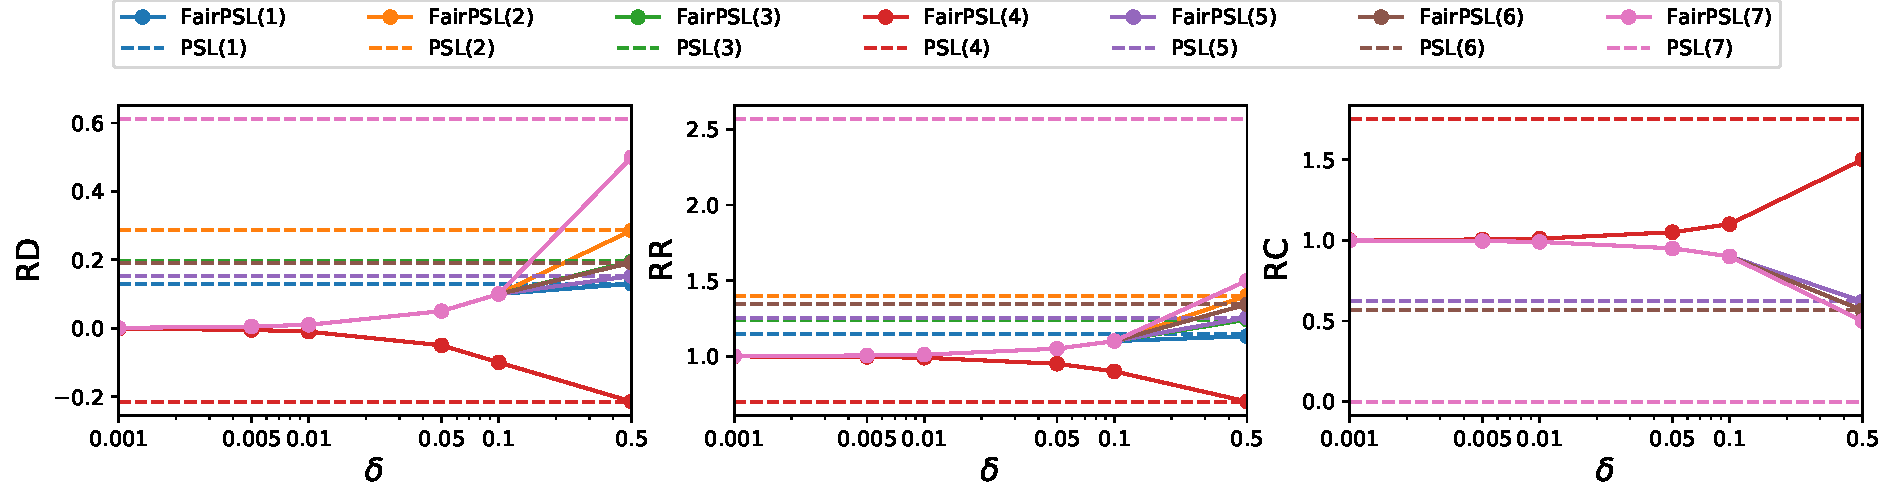
\includegraphics[width=1\linewidth]{figs/results_vis_uni_params.pdf}
\caption{\small Fairness score of predictions obtained by MAP inference of PSL and FairPSL, according to the fairness measures \emph{RD}, \emph{RR}, and \emph{RC}. The labels of datasets are mentioned with parenthesis next to the inference method. The FairPSL values of each measure are obtained by adding the $\delta$-fairness constraint of that measure.\label{fig:results}
}  
\end{figure}

To answer \textbf{Q1}, we run the MAP inference algorithm of PSL and FairPSL on seven synthetic datasets. 
We run the MAP inference of FairPSL multiple times on each dataset: For each of the three fairness measures, we add the corresponding $\delta$-fairness constraint with five thresholds $\{0.001, 0.005, 0.01, 0.05, 0.1, 0.5\}$.

Figure~\ref{fig:results} shows the fairness score of predictions in terms of the three fairness measures. As expected, tighter $\delta$-fairness constraints lead to better scores. Note that the best possible score according to RD is 0, as it computes a difference. Since RR and RC compute ratios, the best possible score according to these measures is 1. In our experiments, with any of these measures, taking $\delta = 0.001$ pushes the score of predictions to its limit.  

The $\delta$-fairness constraints modify the optimization problem of MAP inference by reducing the feasible region to solutions that conform with fairness guarantees. Research question \textbf{Q2} is concerned with the effect of this reduction on the accuracy of predictions. Note that decision quality is the same as the accuracy of predictions. To answer this question, we compare the inferred values for the decision atoms \textit{ToPromote(e)} against their actual values. These values are extracted from the known values of \textit{IsQualified(e)} according to rules 11 and 12 in Table~\ref{tab:pslmodel}. Figure~\ref{fig:accuracy} shows the area under the curve of the receiver operating characteristic~(AUC) of predicting the decision variable in three groups, namely the protected group, the unprotected group (i.e., promotion of the employees who have in-group managers), and all employees. By doing so, we make sure that our fairness constraints do not propagate bias towards either of the populations. Since the results of FairPSL with $\delta$-fairness constraints RR and RC are very similar to the results of RD, we only report the latter here.


\begin{figure}
    \centering
    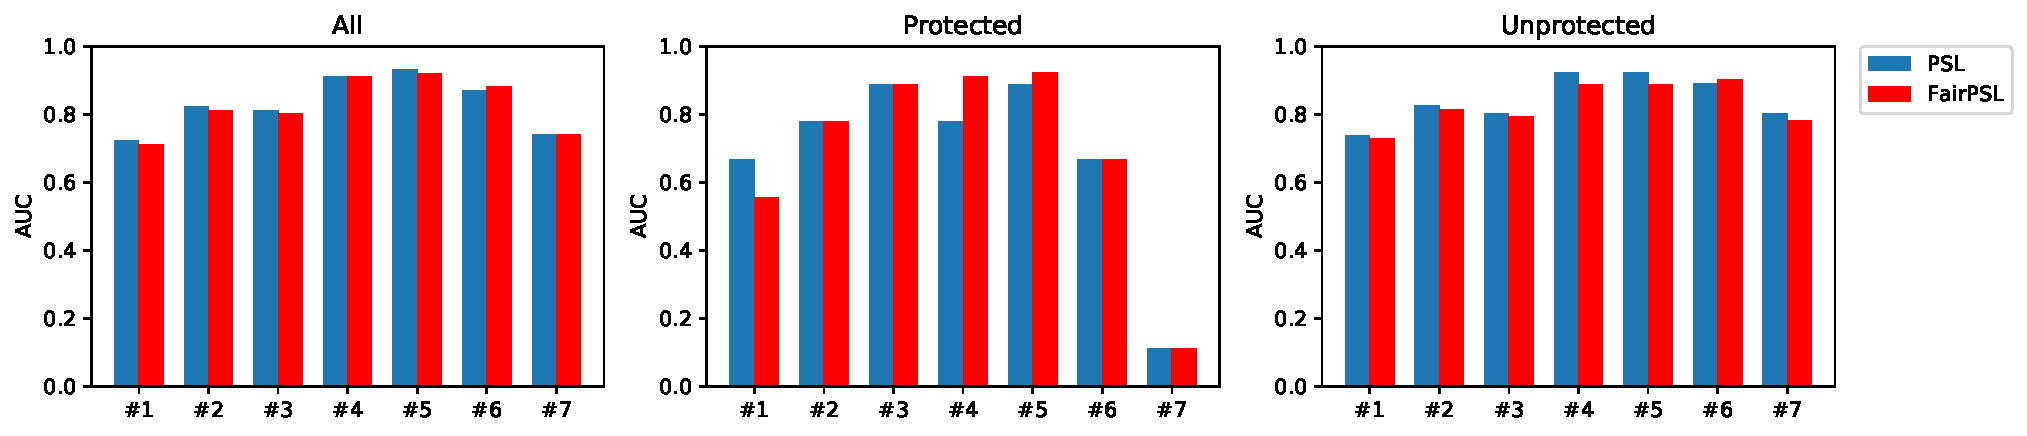
\includegraphics[width=\textwidth]{figs/roc.pdf}
    \caption{\small AUC score of predictions for truth values of unknown atoms \textit{ToPromote(e)} using MAP inference of PSL and FairPSL with $\delta$-fairness constraints $RD$ with $\delta=0.001$.}
    \label{fig:accuracy}
\end{figure}

According to Figure~\ref{fig:accuracy}, the results of both PSL and FairPSL in all seven datasets are close to each other. Note that although fairness may impose a cost in terms of overall accuracy, FairPSL often improves the accuracy of the protected class. Sometimes the overall predictions of FairPSL are even slightly better than PSL (e.g., dataset 6 and 7). As expected, the accuracy of the fourth setting where the opinions are unbiased are similar in both PSL and FairPSL. We observe that prediction of MAP inference for both FairPSL and PSL are similar, thus, in these settings at least, FairPSL guarantees fairness without hurting accuracy. Further investigation is required on the effect of the various ranges of discrimination (i.e., $\theta_1$, $\theta_2$, $\theta_3$, $\theta_4$) on the prediction results of FairPSL.



We also generate various types of organizations in which labels are not uniformly distributed, e.g., one population only occurs at the bottom levels of an organization. While we did not observe any differences in the behavior of our method with respect to accuracy and fairness measure, we found that the degree of discrimination is higher in such organizations. Further investigations on the structure of an organization on discrimination is an interesting direction for future research. 

\section{Conclusion and Future Directions}
\label{sec:conclusion}
Many applications of AI and machine learning affect peoples' lives in important ways. While there is a growing body of work on fairness in AI and ML, it assumes an individualistic notion of fairness.   In this paper, we have proposed a general framework for relational fairness which includes both a rich language for defining discrimination patterns and an efficient algorithm for performing inference subject to fairness constraints. We show our approach enforces fairness guarantees while preserving the accuracy of the predictions. 

There are many avenues for expanding on this work. For example, here we assumed that the discriminative pattern is given, however an automatic mechanism to extract discriminatory situations hidden in a large amount of decision records is an important and required task. Discrimination discovery has been studied for attribute-based fairness~\cite{pedreschi2013discovery}. An interesting next step is discrimination pattern discovery in relational data.

\section*{Acknowledgements}
This work is supported by the National Science Foundation under Grant Numbers CCF-1740850 and IIS-1703331. Golnoosh Farnadi and Behrouz Babaki are  supported by postdoctoral scholarships from IVADO through the Canada First Research Excellence Fund (CFREF) grant.

\begin{thebibliography}{10}
\itemsep=1pt 
\begin{small}

\bibitem{EUlaw}
European union legislation. (a) racial equality directive, 2000; (b) employment
  equality directive, 2000; (c) gender employment directive, 2006; (d) equal
  treatment directive (proposal), 2008.

\bibitem{UKlaw}
{UK} legislation. (a) sex discrimination act, 1975, (b) race relation act,
  1976.

\bibitem{USlaw}
United nations legislation. (a) universal declaration of human rights, 1948,
  (c) convention on the elimination of all forms of racial discrimination,
  1966, (d) convention on the elimination of all forms of discrimination
  against women, 1979.

\bibitem{alshukaili:iswc16}
Duhai Alshukaili, Alvaro A.~A. Fernandes, and Norman~W. Paton.
\newblock Structuring linked data search results using probabilistic soft
  logic.
\newblock In {\em International Semantic Web Conference {(1)}}, volume 9981 of
  {\em Lecture Notes in Computer Science}, pages 3--19, 2016.

\bibitem{bach:jmlr17}
Stephen~H. Bach, Matthias Broecheler, Bert Huang, and Lise Getoor.
\newblock Hinge-loss markov random fields and probabilistic soft logic.
\newblock {\em Journal of Machine Learning Research}, 18:109:1--109:67, 2017.

\bibitem{barocas2016big2}
Solon Barocas and Andrew~D Selbst.
\newblock Big data's disparate impact.
\newblock {\em California Law Review}, 104:671, 2016.

\bibitem{boyd2014networked}
Danah Boyd, Karen Levy, and Alice Marwick.
\newblock The networked nature of algorithmic discrimination.
\newblock In {\em Data and discrimination: Collected essays}, pages 53--57.
  2014.

\bibitem{brewer1979group}
Marilynn~B Brewer.
\newblock In-group bias in the minimal intergroup situation: A
  cognitive-motivational analysis.
\newblock {\em Psychological bulletin}, 86(2):307, 1979.

\bibitem{brewer2007social}
Marilynn~B Brewer.
\newblock The social psychology of intergroup relations: Social categorization,
  ingroup bias, and outgroup prejudice.
\newblock {\em Social Psychology: Handbook of Basic Principles}, 2007.

\bibitem{chouldechova2017fair2}
Alexandra Chouldechova.
\newblock Fair prediction with disparate impact: {A} study of bias in
  recidivism prediction instruments.
\newblock {\em CoRR}, abs/1703.00056, 2017.

\bibitem{dwork2012fairness3}
Cynthia Dwork, Moritz Hardt, Toniann Pitassi, Omer Reingold, and Richard~S.
  Zemel.
\newblock Fairness through awareness.
\newblock In {\em {ITCS}}, pages 214--226. {ACM}, 2012.

\bibitem{ebrahimi:emnlp16}
Javid Ebrahimi, Dejing Dou, and Daniel Lowd.
\newblock Weakly supervised tweet stance classification by relational
  bootstrapping.
\newblock In {\em {EMNLP}}, pages 1012--1017. The Association for Computational
  Linguistics, 2016.

\bibitem{farnadi2018fairness}
Golnoosh Farnadi, Behrouz Babaki, and Lise Getoor.
\newblock Fairness in relational domains.
\newblock In {\em AAAI/ACM Conference on AI, Ethics, and Society (AIES)}, pages
  108--114. ACM, 2018.

\bibitem{feldman2015certifying2}
Michael Feldman, Sorelle~A. Friedler, John Moeller, Carlos Scheidegger, and
  Suresh Venkatasubramanian.
\newblock Certifying and removing disparate impact.
\newblock In {\em {KDD}}, pages 259--268. {ACM}, 2015.

\bibitem{getoor2007introduction}
Lise Getoor and Ben Taskar.
\newblock {\em {Introduction to Statistical Relational Learning}}.
\newblock MIT press Cambridge, 2007.

\bibitem{hardt2016equality3}
Moritz Hardt, Eric Price, and Nati Srebro.
\newblock Equality of opportunity in supervised learning.
\newblock In {\em {NIPS}}, pages 3315--3323, 2016.

\bibitem{kamishima2011fairness}
Toshihiro Kamishima, Shotaro Akaho, and Jun Sakuma.
\newblock Fairness-aware learning through regularization approach.
\newblock In {\em ICDMW}, pages 643--650. {IEEE} Computer Society, 2011.

\bibitem{kouki:recsys15}
Pigi Kouki, Shobeir Fakhraei, James~R. Foulds, Magdalini Eirinaki, and Lise
  Getoor.
\newblock Hyper: {A} flexible and extensible probabilistic framework for hybrid
  recommender systems.
\newblock In {\em RecSys}, pages 99--106. {ACM}, 2015.

\bibitem{counterfactualfairness}
Matt~J. Kusner, Joshua~R. Loftus, Chris Russell, and Ricardo Silva.
\newblock Counterfactual fairness.
\newblock In {\em {NIPS}}, pages 4069--4079, 2017.

\bibitem{Pedreschi:2012}
Dino Pedreschi, Salvatore Ruggieri, and Franco Turini.
\newblock A study of top-k measures for discrimination discovery.
\newblock In {\em {SAC}}, pages 126--131. {ACM}, 2012.

\bibitem{pedreschi2013discovery}
Dino Pedreschi, Salvatore Ruggieri, and Franco Turini.
\newblock The discovery of discrimination.
\newblock In {\em Discrimination and Privacy in the Information Society},
  volume~3 of {\em Studies in Applied Philosophy, Epistemology and Rational
  Ethics}, pages 91--108. Springer, 2013.

\bibitem{ridgeway2004unpacking}
Cecilia~L Ridgeway and Shelley~J Correll.
\newblock Unpacking the gender system: A theoretical perspective on gender
  beliefs and social relations.
\newblock {\em Gender \& society}, 18(4):510--531, 2004.

\bibitem{sridhar:bioinformatics16}
Dhanya Sridhar, Shobeir Fakhraei, and Lise Getoor.
\newblock A probabilistic approach for collective similarity-based drug-drug
  interaction prediction.
\newblock {\em Bioinformatics}, 32(20):3175--3182, 2016.

\bibitem{verma2018fairness2}
Sahil Verma and Julia Rubin.
\newblock Fairness definitions explained.
\newblock In {\em 2018 IEEE/ACM International Workshop on Software Fairness
  (FairWare)}, pages 1--7. IEEE, 2018.

\bibitem{west2014exploiting}
Robert West, Hristo~S. Paskov, Jure Leskovec, and Christopher Potts.
\newblock Exploiting social network structure for person-to-person sentiment
  analysis.
\newblock {\em {TACL}}, 2:297--310, 2014.

\bibitem{zafar2017parity}
Muhammad~Bilal Zafar, Isabel Valera, Manuel Gomez{-}Rodriguez, Krishna~P.
  Gummadi, and Adrian Weller.
\newblock From parity to preference-based notions of fairness in
  classification.
\newblock In {\em {NIPS}}, pages 228--238, 2017.

\bibitem{zemel2013learning}
Richard~S. Zemel, Yu~Wu, Kevin Swersky, Toniann Pitassi, and Cynthia Dwork.
\newblock Learning fair representations.
\newblock In {\em {ICML} {(3)}}, volume~28 of {\em {JMLR} Workshop and
  Conference Proceedings}, pages 325--333. JMLR.org, 2013.

\end{small}
\end{thebibliography}

\end{document}

\end{article}



\begin{article}
{A Human-in-the-loop Perspective on AutoML: Milestones and the Road Ahead}
{Doris Jung-Lin Lee, Stephen Macke, Doris Xin, Angela Lee, Silu Huang, Aditya Parameswaran}
\graphicspath{{submissions/automl/}}
%\documentclass[11pt,dvipdfm]{article}
\documentclass[11pt]{article}
\usepackage{deauthor,times,graphicx} %required
\usepackage{amsmath,amssymb}
\usepackage{multirow}
\usepackage{algorithm}
\usepackage{algpseudocode}
\usepackage{todonotes}
\usepackage{url}

% \graphicspath{{farnadi/}}

\newtheorem{mydef}{\textbf{Definition}}
\newtheorem{myex}{\textbf{Example}}
\newtheorem{mytheorem}{\textbf{Theorem}}


\begin{document}

\title{A Declarative Approach to Fairness in Relational Domains}
\author{Golnoosh Farnadi$^{1,2}$, Behrouz Babaki$^1$, Lise Getoor$^3$\\
$^1$Polytechnique Montr\'{e}al, $^2$ Mila, $^3$ UC Santa Cruz \\
farnadig@mila.quebec, behrouz.babaki@polymtl.ca, getoor@soe.ucsc.edu}

\maketitle

\begin{abstract}
AI and machine learning tools are being used with increasing frequency for decision making in domains that affect peoples' lives such as employment, education, policing and %loan approval
financial qualifications. These uses raise concerns about biases of algorithmic discrimination and have motivated the development of fairness-aware machine learning. However, existing fairness approaches are based solely on attributes of individuals. In many cases, discrimination is much more complex, and taking into account the social, organizational, and other connections between individuals is important. We introduce new notions of fairness that are able to capture the relational structure in a domain. We use first-order logic to provide a flexible and expressive language for specifying complex relational patterns of discrimination. Furthermore, we extend an existing statistical relational learning framework, probabilistic soft logic~(PSL), to incorporate our definition of relational fairness. We refer to this fairness-aware framework FairPSL. FairPSL makes use of the logical definitions of fairnesss but also supports a probabilistic interpretation. In particular, we show how to perform maximum a posteriori~(MAP) inference by exploiting probabilistic dependencies within the domain while avoiding violations of fairness guarantees. Preliminary empirical evaluation shows that we are able to make both accurate and fair decisions.
\end{abstract}

\section{Introduction}
\label{sec:introduction}

Over the past few years, AI and machine learning have become essential components in operations that drive the modern society, e.g., in financial, administrative, and educational spheres. \emph{Discrimination} happens when qualities of individuals which are not relevant to the decision making process influence the decision. Delegating decision making to an automated process raises questions about discriminating against individuals with certain traits based on biases in the data. This is especially important when the decisions have the potential to impact the lives of individuals, for example, the decisions on granting loans, assigning credit, and employment. 

\emph{Fairness} is defined as the absence of discrimination in a decision making process. The goal of \emph{fairness-aware} machine learning is to ensure that the decisions made by an algorithm do not discriminate against a population of individuals~\cite{feldman2015certifying2,boyd2014networked,hardt2016equality3}. Fairness has been well studied in the social sciences and legal scholarship (for an in-depth review see~\cite{barocas2016big2}), and there is emerging work on fairness-aware ML within the AI and computer science communities. For example, fairness through awareness/Lipschitz property~\cite{dwork2012fairness3}, individual fairness~\cite{zemel2013learning}, statistical parity/group fairness~\cite{kamishima2011fairness}, counterfactual fairness~\cite{counterfactualfairness}, demographic parity/disparate impact~\cite{feldman2015certifying2,chouldechova2017fair2}, preference-based fairness~\cite{zafar2017parity}, and equality of opportunity~\cite{hardt2016equality3}.

The existing work in fairness-aware machine learning is based on a definition of discrimination where a decision is influenced by an \emph{attribute} of an individual. An attribute value upon which discrimination is based (such as gender, race, or religion) is called a \emph{sensitive attribute}. The sensitive attribute defines a population of vulnerable individuals known as the \emph{protected group}. A fair decision-making process treats the protected group the same as the \emph{unprotected group}. 

However, in many social contexts, discrimination is the result of complex interactions and can not be described solely in terms of attributes of an individual. For example, consider an imaginary scenario in an organization in which younger female workers who have older male supervisors have lower chances of promotion than their male counterparts.\footnote{Of course, many other patterns may be possible: female bosses may promote female subordinates and discriminate against male workers, or male bosses may promote female employees.  Our goal is to provide a general framework which is able to describe arbitrarily complex discrimination patterns.} 
 This discrimination pattern involves two attributes of the individual (gender and age), a relationship with another individual (supervisor), and two attributes of the second individual. Addressing such complex cases poses two challenges. First, the concepts of discrimination and fairness need to be extended to capture not only attributes of individuals but also the relationships between them. Second, a process is required that ensures that fair decisions are made about individuals who are affected by such patterns. In this paper we address both of these challenges.
We use first-order logic (FOL) to extend the notion of fairness to the relational setting. FOL is an expressive representation for relational problems which is also widely used for learning in relational domains. Moreover, we extend an existing framework for statistical relational learning~\cite{getoor2007introduction} called probabilistic soft logic (PSL)\footnote{http://psl.linqs.org/}~\cite{bach:jmlr17}. PSL combines logic and probability for learning and reasoning over uncertain relational domains. One of the most common reasoning tasks in PSL is called maximum a posteriori (MAP) inference, which is performed by finding the most probable truth values for unknowns over a set of given evidence. We develop a new MAP inference algorithm which is able to maximize the a posteriori values of unknown variables \emph{subject to} fairness guarantees. An early version of this paper which this work builds upon and extends appeared in~\cite{farnadi2018fairness}.

\looseness-1
Our contributions are as follows: 1) we propose fairness-aware machine learning for the relational setting; 2) we extend PSL into a fairness-aware framework called FairPSL which can represent the logical definition of fairness; 3) we develop a new MAP inference algorithm which is able to maximize the posteriori values of unknown variables \emph{subject to} fairness guarantees; 4) we empirically evaluate our proposed framework on synthetic data. 

\section{Motivation}
\label{sec:motivation}

Discrimination in social contexts have been studied in the field of social psychology~\cite{brewer2007social,brewer1979group,ridgeway2004unpacking}. There is a large literature on various aspects of relational bias in social contexts such as \emph{in-group-out-group bias}, \emph{gender bias}, and \emph{ethnicity-based favoritism} that can result in discrimination. 
As an example, consider gender bias in the workplace that reflects stereotypically masculine criteria and male-based favoritism. Such gender bias 
typically places women in lower positions and negatively impacts their opportunities. Further, lack of women in leadership positions may affect the promotion of women and results in a glass ceiling that keeps women from rising beyond a certain level in the hierarchy. This scenario shows that considering  protected attributes such as gender is not always sufficient to detect the source of bias and avoid discrimination, one also has to consider the relational information, in this case the organization hierarchy. Note that this can be generalized to any ingroup/outgroup scenario where the sensitive attribute could be race, religion, age, marital-status, etc.

The existing work on designing fair algorithms in machine learning exclusively focuses on \emph{attribute-based fairness}, which is based on the following assumptions: First, there is an assumption that the individuals (sometimes referred to as units or entities) are independent and described by simple attribute vectors. Second, the group for which one wishes to ensure fairness (known as the \emph{protected group}) is defined on the basis of some attribute values. Finally, there is a decision that is associated with each individual, and the goal is to ensure that members of the protected group are subject to a fair decision (we discuss different fairness measures in Section~\ref{sec:fairnessmeasure}).  We illustrate  attribute-based fairness in the following example. 

\begin{myex}[Loan Processing]
\label{ex:loan}
A bank bases its decisions about granting a loan on attributes of the applicant. The goal is to decide whether to grant a loan to an applicant using a predictive model. The bank needs to ensure that the obey fair lending practices and ensure that gender, race, sexual orientation of applicants has no influence on the decision. In this scenario, the protected group is the historically disadvantaged applicants.  
\end{myex}
The current fairness-aware machine learning techniques are not capable of modeling relations and hence cannot be used to make the decision making model fair. However, in many decision making scenarios, especially in social and organizational settings, the domain is relational, and the protected group itself might be best represented using a relational definition. We illustrate this setting in the following scenario:
\begin{myex}[Performance Review]
\label{ex:review}
Consider an organization where decisions about the promotion of employees is based on two criteria: 1) an objective performance measure, and 2) the opinion of their direct and indirect managers above them. The opinions are inferred from the performance reviews which are collected periodically. Not every manager can submit a review for all its subordinates, this is especially the case for top-level managers who have a large number of subordinates. Hence, the opinions of managers are collectively inferred from the opinions of their sub-ordinates. However, some employees may be biased, and judge other employees unfavorably, by favoring employees who are similar to themselves (same gender, race, religion, etc.) over employees who are dissimilar. The organization needs to ensure that promotion of employees do not have any relational bias caused by in-group-out-group favoritism.

\end{myex}
Example~\ref{ex:review} describes a prediction problem over a database that consists of relations between employees. Such prediction tasks are best handled by techniques from the relational learning domain. To ensure fair prediction in such settings, we need to extend the notion of \emph{attribute-based fairness} to \emph{relational fairness}. Throughout this paper, we use the performance review problem as a running example for relational fairness.

\section{Fairness Formalism}
\label{sec:formulation}

A representation that can describe different types of entities and different relationships between them is called relational. In this section, we use first-order logic to define relational fairness. We employ first-order logic as an expressive representation formalism which can represent objects and complex relationships between them. We start by defining an atom:

\begin{mydef}[Atom]
An atom is an expression of the form $P(a_1, a_2, \ldots, a_n)$ where each argument $a_1, a_2,$ $\ldots,$ $a_n$ is either a constant or a variable. The finite set of all possible substitutions of a variable to a constant for a particular variable $a$ is called its \textit{domain} $D_{a}$. If all variables in $P(a_1, a_2, \ldots, a_n)$ are substituted by some constant from their respective domain, then we call the resulting atom a \textit{ground atom}. 
\end{mydef}

\begin{myex}
In our loan processing problem (Example~\ref{ex:loan}), we can represent applicants' attributes by atoms. For instance, atom $Female(v)$ indicates whether or not applicant $v$ is female. Similarly, we can represent relations with atoms. In the performance review problem in Example~\ref{ex:review} the atom $Manager(m,e)$ indicates whether or not employee $m$ is a direct or indirect manager of employee $e$.
\end{myex}

The relational setting provides the flexibility to express complex definitions with formulae.

\begin{mydef}[Formula] 
A formula is defined by induction: every atom is a formula. If $\alpha$ and $\beta$ are formulae, then $\alpha \vee \beta$, $\alpha \wedge \beta$, $\neg \alpha$, $\alpha \rightarrow \beta$ are formulae. If $x$ is a variable and $\alpha$ is a formula, then the quantified expressions of the form $\exists x$ $\alpha$ and $\forall x$ $\alpha$ are formulae.    
\end{mydef}

To characterize groups of individuals based on a formula, we define the notion of \emph{population}.

\begin{mydef}[Population]
We denote formula $F$ which has only one free variable $v$ (i.e., other variables in $F$ are quantified) by $F[v]$. The population defined by $F[v]$ is the set of substitutions of $v$ for which $F[v]$ holds.   
\end{mydef}


\begin{myex}
\label{ex:disformula}
Consider the formula $F[v] := \forall u, \, \textit{Manager}(u,v) \rightarrow \neg \textit{SameGroup}(u, v)$. The population specified by this formula is the set of individuals all of whose managers belong to a group different from theirs. 
\end{myex}

The truth value of a formula is derived from the truth value of atoms that it comprises, according to the rules of logic. Each possible assignment of truth values to ground atoms is called an \emph{interpretation}. 


\begin{mydef}[Interpretation]
An interpretation $I$ is a mapping that associates a truth value $I(P)$ to each ground atom $P$. For Boolean truth values, $I$ associates true to 1 and false to 0 truth values. For soft logic (see Definition~\ref{def:softlogic}) $I$ maps each ground atom $P$ to a truth value in interval $[0, 1]$.
\end{mydef}

In attribute-based fairness, it is assumed that there is a certain attribute of individuals, i.e, the sensitive attribute,  that we do not want to affect a decision. Gender, race, religion and marital status are examples of sensitive attributes. Discrimination has been defined in social science studies as a treatment in favor or against a group of individuals given their sensitive attribute. This group of individuals is the protected group. 

In a relational setting, both the sensitive attributes of an individual and their participation in various relations may have an undesired effect on the final decision. We characterize the protected group in a relational setting by means of a population. In practice, we are often interested in maintaining fairness for a specific population such as applicants, students, employees, etc. This population is then partitioned into the protected and unprotected groups. We define a \emph{discriminative pattern} which is a pair of formulae to capture these groups: 1) $F_1[v]$: to specify the difference between the protected and unprotected groups and 2) $F_2[v]$: to specify the population over which we want to maintain fairness. 

\begin{mydef}[Discriminative pattern]
A discriminative pattern is a pair $\textit{DP}[v]:=(F_1[v], F_2[v])$ , where $F_1[v]$ and $F_2[v]$ are formulae.
\end{mydef}

\begin{myex}
\label{ex:pattern}
The two formulae in the discrimination pattern $\textit{DP}[v]:= \big((\forall u, \,  \textit{Manager}(u,v) \rightarrow  \neg \textit{SameGroup}(u, v)),$ $\textit{Employee}(v)\big)$ specify two populations, namely all employees and those employees who belong to a group different from their managers.
\end{myex}

Given the definition of the discriminative pattern, we have a rich language to define the scope of the protected and unprotected groups in a relational setting.

\begin{mydef}[Protected group] Given an interpretation $I$, the protected group is a population of the form:
{$$PG :=\{ v : F_1[v] \wedge F_2[v]\}$$}
which is defined as the set of all instances hold for variable $v$ for which $F_1[v] \wedge F_2[v]$ is true under interpretation $I$, that is, $I(F_1[v] \wedge F_2[v]) = 1$. 
Similarly, the \emph{unprotected group} is a population of the form: 
{$$UG := \{ v : \neg F_1[v] \wedge  F_2[v]\}$$}
which is defined as the set of all instances hold for variable $v$ 
for which $I(\neg F_1[v] \wedge F_2[v]) = 1$. 
\end{mydef}

\begin{myex}
The protected group of the discrimination pattern specified in Example~\ref{ex:pattern} is {$PG := \big\{ v : \big(\forall u, \,$ $ \textit{Manager}(u, v) \rightarrow \neg \textit{SameGroup}(u, v)\big) \wedge \textit{Employee}(v) \big\}$} and the unprotected group is {$UG :=  \big\{ v:  \big(\exists u, \, \textit{Manager}(u,v) \wedge \textit{SameGroup}(u, v)\big) \wedge \textit{Employee}(v) \big\}$}. This means our protected group is the set of employees belonging to a group different from their managers,
and our unprotected group consists of other employees. 
\end{myex}

Discrimination is defined in terms of a treatment or decision that distinguishes between the protected and unprotected groups. Here we define the \emph{decision} atom.
\begin{mydef}[Decision atom] A decision atom $d(v)$ is an atom containing exactly one variable $v$ that specifies a decision affecting the protected group which is defined either by law or end-user.
\end{mydef}
\begin{myex}
The decision atom ${\textit ToPromote}(v)$ indicates whether or not $v$ receives a promotion.
\end{myex}

Note that the fairness formulation in this section is designed for the relational setting, however relational fairness subsumes the attribute-based fairness such that: a sensitive attribute is defined by an atom with one argument and $F_2[v]$ in discrimination pattern is $\textit{Applicant}(v)$. For example, discrimination pattern of our loan processing problem in Example~\ref{ex:loan} is of the form $\textit{DP} := ( \textit{Female}(v), \textit{Applicant}(v))$ that denotes female applicants as the protected group (i.e., $PG :=  \{ v: \textit{Female}(v) \}$) and male applicants as the unprotected group (i.e., $UG := \{ v: \neg \textit{Female}(v)\}$).


\section{Fairness Measures}
\label{sec:fairnessmeasure}

Over the past few years, many fairness measures have been introduced~\cite{verma2018fairness2}. An important class of these measures are \emph{group fairness} measures which quantify the inequality between different subgroups. Some of the most popular measures in this class include \emph{equal opportunity}, \emph{equalized odds}, and \emph{demographic parity}~\cite{hardt2016equality3}. In this paper we restrict our focus to the latter. In an attribute-value setting, demographic parity means that the decision should be independent of the protected attributes. Assume that binary variables $A$ and $C$ denote the decision and protected attributes, and the preferred value of $A$ is one. Demographic parity requires that:

\begin{equation*}
    P(A=1 | C=0) = P(A=1 | C=1)
\end{equation*}

We will now generalize this measure to the relational setting using the notations defined in Section~\ref{sec:formulation}. Let $a$ and $c$ denote the counts of denial (i.e., negative decisions) for protected and unprotected groups, and $n_{1}$ and $n_{2}$ denote their sizes, respectively. Given the decision atom $d(v)$, discriminative pattern $\textit{DP}(F_1[v], F_2[v])$, and interpretation $I$, these counts are computed by the following equations: 
{
\begin{flalign}
    & a \equiv \sum_{v \in D_v} I\big( \neg d(v) \wedge  F_1[v] \wedge F_2[v]) \label{eq:a}\\
    & c \equiv \sum_{v \in D_v} I\big( \neg d(v) \wedge  \neg F_1[v] \wedge  F_2[v]) \label{eq:c}\\
    & n_{1} \equiv \sum_{v \in D_v} I\big(F_1[v] \wedge F_2[v]) \label{eq:n1}\\
    & n_{2} \equiv \sum_{v \in D_v} I\big(\neg F_1[v] \wedge  F_2[v]) \label{eq:n2}
\end{flalign}}
The proportions of denying for protected and unprotected groups are $p_1 = \frac{a}{n_1}$ and $p_2 = \frac{c}{n_2}$, respectively. There are a number of data-driven measures~\cite{Pedreschi:2012} which quantify demographic disparity and can be defined in terms of $p_1$ and $p_2$:
\begin{itemize}
    \item \textbf{Risk difference}: $RD = p_1 - p_2$, also known as absolute risk reduction. 
    \item \textbf{Risk Ratio}: $RR = \frac{p_1}{p_2}$, also known as relative risk. 
    \item \textbf{Relative Chance}: $RC = \frac{1 - p_1}{1 - p_2}$ also, known as selection rate.
\end{itemize}
These measures have been used in the legal systems of European Union, UK, and US~\cite{EUlaw,UKlaw,USlaw}. Notice that RR is the ratio of the proportion of benefit denial between the protected and unprotected groups, while RC is the ratio of the proportion of benefit granted. Finally, we introduce the notion of $\delta$-fairness.

\begin{mydef}[$\delta$-fairness]
If a fairness measure for a decision making process falls within some $\delta$-window, then the process is \emph{$\delta\text{-fair}$}. Given $0 \leq \delta \leq 1$, the  $\delta$-windows for measures RD/RR/RC are defined as:
{\begin{flalign*}
	     - \delta \leq &RD \leq \delta \\
	     1- \delta \leq &RR \leq 1+ \delta\\
	     1- \delta \leq &RC \leq 1+ \delta
	\end{flalign*}}
\end{mydef}

To overcome the limitations of attribute-based fairness, we introduce a new statistical relational learning~(SRL) framework~\cite{getoor2007introduction} suitable for modelling fairness in relational domain. In the next section, we review probabilistic soft logic~(PSL). We then extend PSL with the definition of relational fairness introduced above in Section~\ref{sec:fairMAP}. Our fairness-aware framework, ``FairPSL'', is the first SRL framework that performs fair inference. 

\section{Background: Probabilistic Soft Logic}
\label{sec:psl}

In this section, we review the syntax and semantics of PSL, and in the next section we extend MAP inference in PSL with fairness constraints to define MAP inference in FairPSL.

PSL is a probabilistic programming language for defining hinge-loss Markov random fields~\cite{bach:jmlr17}. Unlike other SRL frameworks whose atoms are Boolean, atoms in PSL can take continuous values in the interval $[0,1]$. PSL is an expressive modeling language that can incorporate domain knowledge with first-order logical rules and has been used successfully in various domains, including bioinformatics~\cite{sridhar:bioinformatics16}, recommender systems~\cite{kouki:recsys15}, natural language processing~\cite{ebrahimi:emnlp16}, information retrieval~\cite{alshukaili:iswc16}, and social network analysis~\cite{west2014exploiting}, among many others. 
 
A PSL model is defined by a set of first-order logical rules called \emph{PSL rules}.

\begin{mydef} [PSL rule] a PSL rule $r$ is an expression of the form:
{\begin{equation}
\lambda_{r}: T_1 \land T_2 \land \ldots \land T_w \rightarrow H_1 \vee H_2 \vee \ldots \vee H_l
\end{equation}}

where { $T_1, T_2, \ldots, T_w, H_1, H_2, \ldots, H_l$} are atoms or negated atoms and { $\lambda_{r} \in \mathbb{R}^{+} \cup \infty$} is the weight of the rule $r$.  We call { $T_1 \land T_2 \land \ldots \land T_w$} the body of $r$ ($r_{body}$), and { $H_1 \vee H_2 \vee \ldots \vee H_l$} the head of $r$ ($r_{head}$).
\end{mydef}


Since atoms in PSL take on continuous values in the unit interval $[0,1]$, next we define soft logic to calculate the value of the PSL rules under an interpretation $I$.

\begin{mydef}[Soft logic]
\label{def:softlogic}
The ({$\tilde{\wedge}$}) and ({$\tilde{\vee}$}) and negation ({$\tilde{\neg}$}) are defined as follows. For {$m, n \in [0,1]$} we have: {$m \tilde{\wedge} n = \max(m+n -1, 0)$}, {$m \tilde{\vee} n = \min(m+n , 1)$} and {$\tilde{\neg} m = 1 - m$}. The $\, \tilde{} \,$ indicates the relaxation over Boolean values.
\end{mydef}

The probability of truth value assignments in PSL is determined by the rules' \emph{distance to satisfaction}.

\begin{mydef}[The distance to satisfaction]
The distance to satisfaction $d_{r}(I)$ of a rule $r$ under an interpretation $I$ is defined as:
{
\begin{equation}
d_{r}(I) = \max\{0, I(r_{body})-I(r_{head})\}
\end{equation}}
\end{mydef}

By using Definition~\ref{def:softlogic}, one can show that the closer the interpretation of a grounded rule $r$ is to 1, the smaller its distance to satisfaction. A PSL model induces a distribution over interpretations $I$. Let $R$ be the set of all grounded rules, then the probability density function is:
{
\begin{equation}
f(I) ={\frac{1}{Z}} \exp[-\sum_{r\in R} \lambda_{r}(d_{r}(I))^p]
\label{eq:potential}
\end{equation}
}
\noindent where { $\lambda_{r}$} is the weight of rule $r$, {
$Z = \int_{I} \exp[ -\sum_{r\in R} \lambda_{r}(d_{r}(I))^p]$
} is a normalization constant, and { $p \in \{1,2\}$} provides a choice of two different loss functions, $p=1$ (i.e., linear), and $p=2$ (i.e, quadratic). These probabilistic models are instances of hinge-loss Markov random fields~(HL-MRF)~\cite{bach:jmlr17}. The goal of maximum a posteriori (MAP) inference is to find the most probable truth assignments $I_{\textit{MPE}}$ of unknown ground atoms given the evidence which is defined by the interpretation $I$. Let $X$ be all the evidence, i.e., $X$ is the set of ground atoms such that $\forall x \in X, I(x)$ is known, and let $Y$ be the set of ground atoms such that $\forall y \in Y, I(y)$ is unknown. Then we have
{
\begin{equation}
I_{\textit{MAP}}(Y) = \textit{arg}\max_{I(Y)} P(I(Y)|I(X))
\end{equation}}
Maximizing the density function in Equation~\ref{eq:potential} is equivalent to minimizing the weighted sum of the distances to satisfaction of all rules in PSL. 

\begin{table*}[t]
    \centering
    \begin{tabular}{|lll|}
    \hline
    &&\\
    $R1$ & $\lambda_1$ &: $\textit{IsQualified}(e) \rightarrow \textit{HighPerformance}(e)$ \\
    $R2$ & $\lambda_1$ &: $\neg \textit{IsQualified}(e) \rightarrow \neg \textit{HighPerformance}(e)$ \\
    $R3$ & $\infty$ &: $\textit{PositiveReview}(e1, e2) \rightarrow \textit{PositiveOpinion}(e1, e2)$ \\
    $R4$ & $\infty$ &: $\neg \textit{PositiveReview}(e1, e2) \rightarrow \neg \textit{PositiveOpinion}(e1, e2)$ \\
    $R5$ & $\lambda_1$ &: $\textit{PositiveOpinion}(e1, e2) \wedge \textit{Manager}(m, e1) \rightarrow \textit{PositiveOpinion}(m, e2)$ \\
    $R6$ & $\lambda_1$ &: $\neg \textit{PositiveOpinion}(e1, e2) \wedge \textit{Manager}(m, e1) \rightarrow \neg \textit{PositiveOpinion}(m, e2)$ \\
    $R7$ & $\lambda_1$ &: $\textit{PositiveOpinion}(m, e) \wedge \textit{Manager}(m, e) \rightarrow \textit{IsQualified}(e)$ \\
    $R8$ & $\lambda_1$ &: $\neg \textit{PositiveOpinion}(m, e) \wedge \textit{Manager}(m, e) \rightarrow \neg \textit{IsQualified}(e)$ \\
    $R9$ &  $\lambda_1$ &: $\neg \textit{ToPromote}(e)$\\
    $R10$ & $\infty$ &: $\textit{IsQualified}(e) \rightarrow \textit{ToPromote}(e)$ \\
    $R11$ & $\infty$ &: $\neg \textit{IsQualified}(e) \rightarrow \neg \textit{ToPromote}(e)$ \\
    &&\\
    \hline
    \end{tabular}
    \caption{\small A simplified PSL model for the \emph{Performance Reviewing} problem}
    \label{tab:pslmodel}
\end{table*}

\begin{myex}
\label{ex:pslmodel}
The simplified PSL model for the performance reviewing problem in Example\ref{ex:review} is given in Table~\ref{tab:pslmodel}. The goal of MAP inference for this problem is to infer employees to promote. We simplified the model by assigning the same weight to all soft rules (i.e., $\lambda_i= 1$ where $i=\{1,2,5,6,7,8,9\}$). Below we explain the meaning of each rule in the model.

Rule $R1$ indicates that qualified employees have high performance and similarly rule $R2$ expresses that a negative qualification of employees is derived from their low performance. Rules $R5$ and $R6$ presents the propagation of opinion from bottom to top of the organizational hierarchy, i.e., managers have similar opinions towards employees given the opinions of their sub-ordinate managers. And rules $R7$ and $R8$ indicate that the positive/negative opinion of direct/indirect managers derive from the qualification of an employee. Rule $R9$ indicates the prior that not all employees get promoted. We also have four hard constraints (i.e., rules $R3$, $R4$, $R10$ and $R11$) where the weight of the rules are $\infty$. Rules $R3$ and $R4$ indicate that submitted positive/negative reviews should reflect positive/negative opinions. And two rules $R10$ and $R11$ show that a highly qualified employee should get promoted. 
\end{myex}

\section{Fairness-aware PSL (FairPSL)}
\label{sec:fairMAP}

The standard MAP inference in PSL aims at finding values that maximize the conditional probability of unknowns. Once a decision is made according to these values, one can use the fairness measure to quantify the degree of discrimination. A simple way to incorporate fairness in MAP inference is to add the $\delta$-fairness constraints to the corresponding optimization problem.   

Consider risk difference, $\textit{RD}$, where $\textit{RD} \equiv \frac{\mathbf{a}}{n_1} - \frac{\mathbf{c}}{n_2}$. The $\delta$-fairness constraint $-\delta \leq \textit{RD} \leq \delta$ can be encoded as the following constraints:
{\begin{align}
    & n_2 \mathbf{a} - n_1 \mathbf{c} - n_1 n_2 \delta \leq 0 \label{eq:RD1}\\
    & n_2 \mathbf{a} - n_1 \mathbf{c} + n_1 n_2 \delta \geq 0
\end{align}}
Similarly, from $\textit{RR} \equiv \frac{\mathbf{a} / n_1}{\mathbf{c} / n_2}$ and the $\delta$-fairness constraint $1 - \delta \leq \textit{RR} \leq 1 + \delta$ we obtain:
{\begin{align}
    & n_2 \mathbf{a} - (1 + \delta) n_1 \mathbf{c} \leq 0 \\
    & n_2 \mathbf{a} - (1 - \delta) n_1 \mathbf{c} \geq 0
\end{align}}
And finally, $\textit{RC} \equiv \frac{1 - \mathbf{a} / n_1}{1 - \mathbf{c} / n_2}$ and the $\delta$-fairness constraint $1 - \delta \leq \textit{RC} \leq 1 + \delta$ gives:
{ \begin{align}
    & - n_2 \mathbf{a} + (1 + \delta) n_1 \mathbf{c} - \delta n_1 n_2 \leq 0 \\
    & - n_2 \mathbf{a} + (1 - \delta) n_1 \mathbf{c} + \delta n_1 n_2 \geq 0 \label{eq:RC2}
\end{align}}
A primary advantage of PSL over similar frameworks is that its MAP inference task reduces to a convex optimization problem which can be solved in polynomial time. To preserve this advantage, we need to ensure that the problem will remain convex after the addition of $\delta$-fairness constraints. 

\begin{mytheorem}
The following condition is sufficient for preserving the convexity of MAP inference problem after addition of $\delta$-fairness constraints: The formulae $F_1[v]$ and $F_2[v]$ do not contain an atom $y \in Y$ and all atoms in $F_1[v]$ and $F_2[v]$ have values zero or one.
\end{mytheorem}
\begin{proof}
Since $I(F_1[v])$ and $I(F_2[v])$ do not depend on $I(Y)$, the values $n_{1}$ and $n_{2}$ are constants that can be computed in advance. Let us define the sets $D_v^a = \{ v \in D_v : F_1[v] \wedge F_2[v] \, \text{is true} \}$ and $D_v^c = \{ v \in D_v : \neg F_1[v] \wedge F_2[v] \, \text{is true} \}$. Since $F_1[v]$ and $F_2[v]$ can be only zero or one, we can rewrite the equations~\ref{eq:a} and \ref{eq:c} as:
{
\begin{align*}
    & \mathbf{a} = \sum_{v \in D_v^a} I(\neg d(v)) = |D_v^a| - \sum_{v \in D_v^a} I(d(v))\\
    & \mathbf{c} = \sum_{v \in D_v^c} I(\neg d(v)) = |D_v^c| - \sum_{v \in D_v^c} I(d(v))
\end{align*}}
\noindent which indicates that $\mathbf{a}$ and $\mathbf{c}$ can be expressed as linear combinations of variables in the optimization problem. This means that constraints~\ref{eq:RD1}-\ref{eq:RC2} are linear. Hence, addition of these constraints preserves the convexity of the optimization problem. 
\end{proof}

\section{Experiments}
\label{sec:experiment}

\begin{figure}
  \begin{minipage}[c]{0.6\textwidth}
    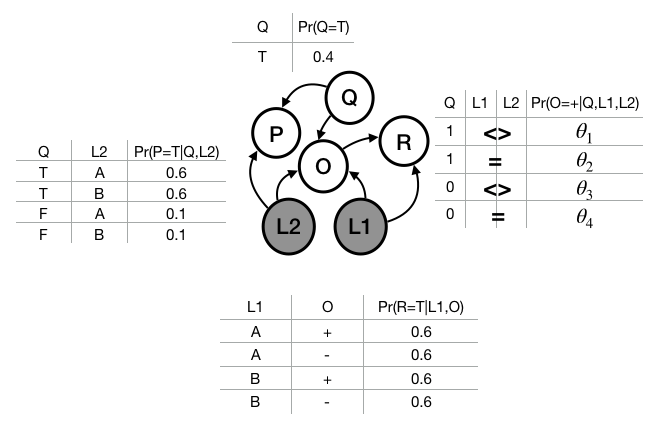
\includegraphics[width=\textwidth]{figs/BN.png}
  \end{minipage}\hfill
  \begin{minipage}[c]{0.45\textwidth}
    \caption{
        \small The model used for generating the datasets. There are four binary random variables, P, Q, O, and R. \textbf{P}: indicates whether or not the employee has high performance; \textbf{Q}: indicates whether or not an employee has high qualification; \textbf{O}: indicates whether or not the colleague submits the positive opinion towards the employee;  \textbf{R}: indicates whether or not the colleague has a positive opinion towards the employee;  \textbf{L1, L2}: indicates the label of the review provider and review receiver (observed).
    } \label{fig:BN}
  \end{minipage}
\end{figure}

We show the effectiveness of FairPSL by performing an empirical evaluation. We investigate two research questions in our experiments:
\begin{description}
\item[Q1] What is the effect of the fairness threshold $\delta$ on the fairness measures $RD/RC/RR$?
\item[Q2] How is decision quality affected by imposing $\delta$-fairness constraints?
\end{description}

Note that although we present the result for specific parameters of the framework in this section, we ran extensive analysis and the results we present are representative. We implemented the MAP inference routines of PSL and FairPSL in Python, using Gurobi-8.1\footnote{\url{www.gurobi.com}} as the backend solver. The FairPSL code, code for the data generator and data is publicly available\footnote{https://github.com/gfarnadi/FairPSL}. 

\subsection{Data generation}
  
We evaluate the FairPSL inference algorithm on synthetic datasets representing the performance review scenario (introduced in Example~\ref{ex:review}). The organization hierarchy is generated synthetically. 
The organization hierarchy generator is parameterized by two numbers: the number of employees in the organization ($n$) and the number of employees managed by each manager ($k$). Each employee is randomly assigned with a label \emph{A} or \emph{B}. An examples organization hierarchy with $n$=50 and $k$=3 is shown in Figure~\ref{fig:hierachy}.

\begin{figure}
  \begin{minipage}[c]{0.3\textwidth}
    \caption{
        \small An example of an organizational hierarchy with five levels and 50 employees with k=3. Each employee either has label A (shown with grey) or B (shown with white).
    }\label{fig:hierachy} 
	\end{minipage} \hfill
    \begin{minipage}[c]{0.7\textwidth}
    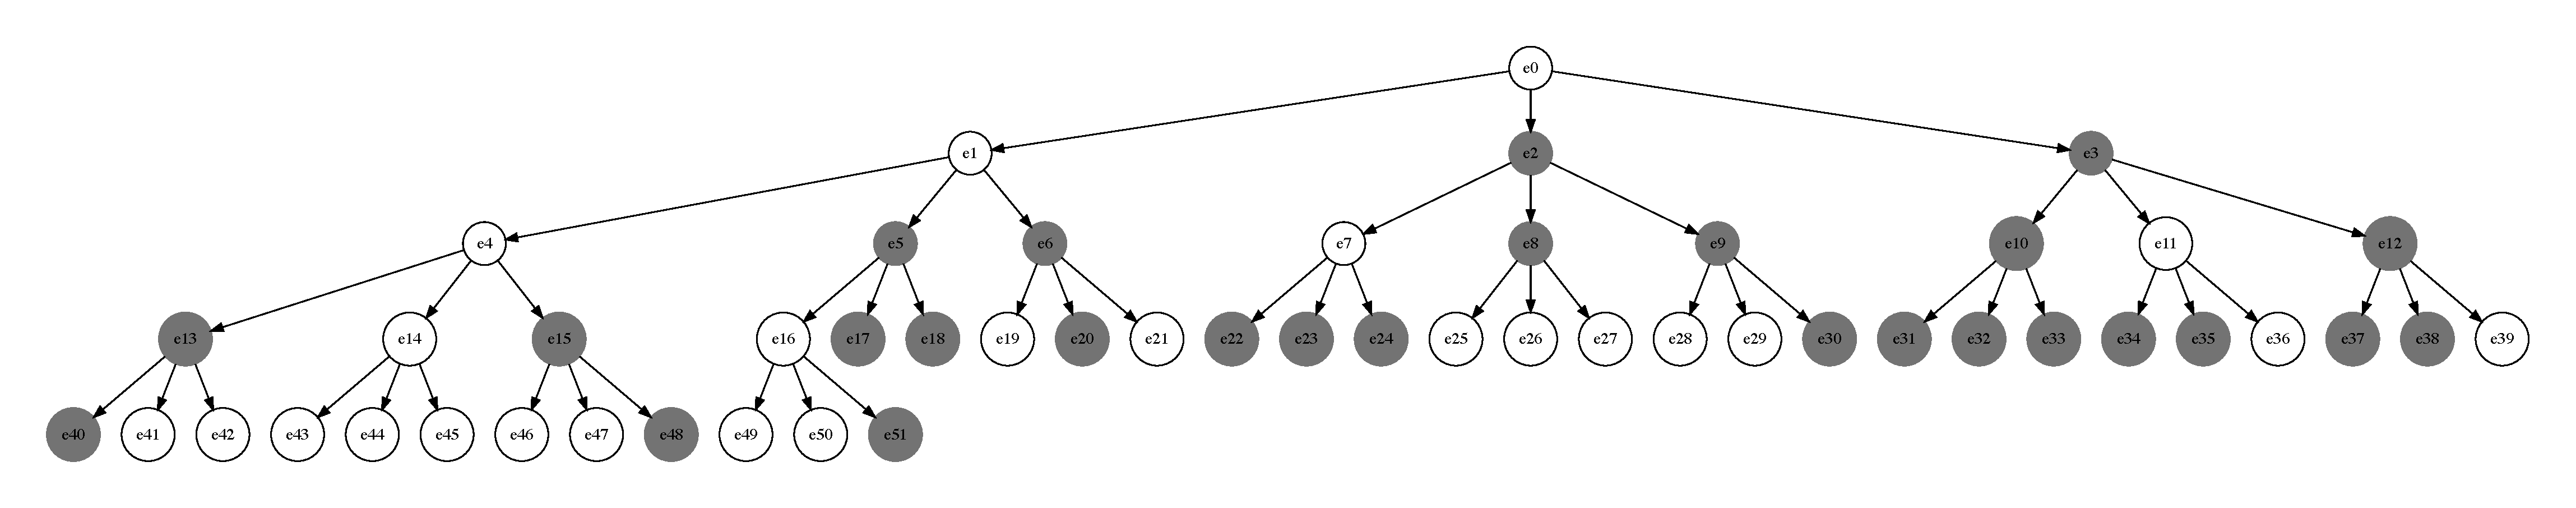
\includegraphics[width=\textwidth]{figs/Uni-hierachy.pdf}
  \end{minipage}
\end{figure}

For each employee, we use the generative model of Figure~\ref{fig:BN} to draw assignments for all the random variables. We assume that only $40\%$ of employees are qualified for promotion and regardless of their labels, employees submit only $60\%$ of their opinions. In addition, due to various personal and environmental factors, only $60\%$ of high quality employees perform well while $10\%$ of low quality employees also perform well regardless of their labels. Note that these numbers are not specific and just chosen for the framework to serve as a representative setting and a proof of concept. The conditional probability table for the opinion variable $O$ is parameterized by four values $(\theta_1, \theta_2, \theta_3, \theta_4)$ which together determine the degree of discrimination against the protected group. Since other parameters in the Bayesian network did not have a direct effect on the degree of discrimination, we fixed them to arbitrary values. 

The results presented in this section are based on an organization hierarchy  with $100$ employees where $k=5$. However, the results of the framework are not sensitive to the settings as we test the framework with various organization sizes ranging from $50$ to $500$ employees and various degree for $k$ ranging from $3$ to $10$. We generated seven datasets given the organization hierarchy using different values for the $\theta$ parameters: $(0.0,1.0,0.0,0.0)$, $(0.33,1.0,0.0,0.0)$, $(0.66,1.0,0.0,0.0)$, $(1.0,1.0,0.0,0.0)$, $(1.0,1.0,0.0,0.33)$, $(1.0,1.0,0.0,0.66)$, $(1.0,1.0,0.0,1.0)$. 
 
In the first three settings the discrimination originates from negative opinions towards qualified outgroup employees. The first setup is an extreme case where the opinion towards outgroup employees is always negative. The discrimination in the last three settings originates from positive opinions towards unqualified ingroup employees. The last setup is an extreme case where the opinion towards ingroup employees is always positive. The fourth setup represent unbiased opinions where employees are treated similarly based on their qualification. 

\paragraph{MAP Inference} We use the model presented in Table~\ref{tab:pslmodel} for MAP inference in PSL and FairPSL (recall that in FairPSL, the $\delta$-fairness constraints corresponding to one of the fairness measures are also added to the model). The observed atoms are $\textit{Manager(m,e)}$, $\textit{PositiveReview(e1,e2)}$ and labels of all employees. The truth values for all other atoms are obtained via MAP inference. We use the truth values obtained for the decision atoms $\textit{ToPromote(e)}$ to compute the fairness measures. We defined the discriminative pattern, and the protected and unprotected groups of this problem in Section~\ref{sec:formulation}.


\subsection{Evaluation results}

\begin{figure}
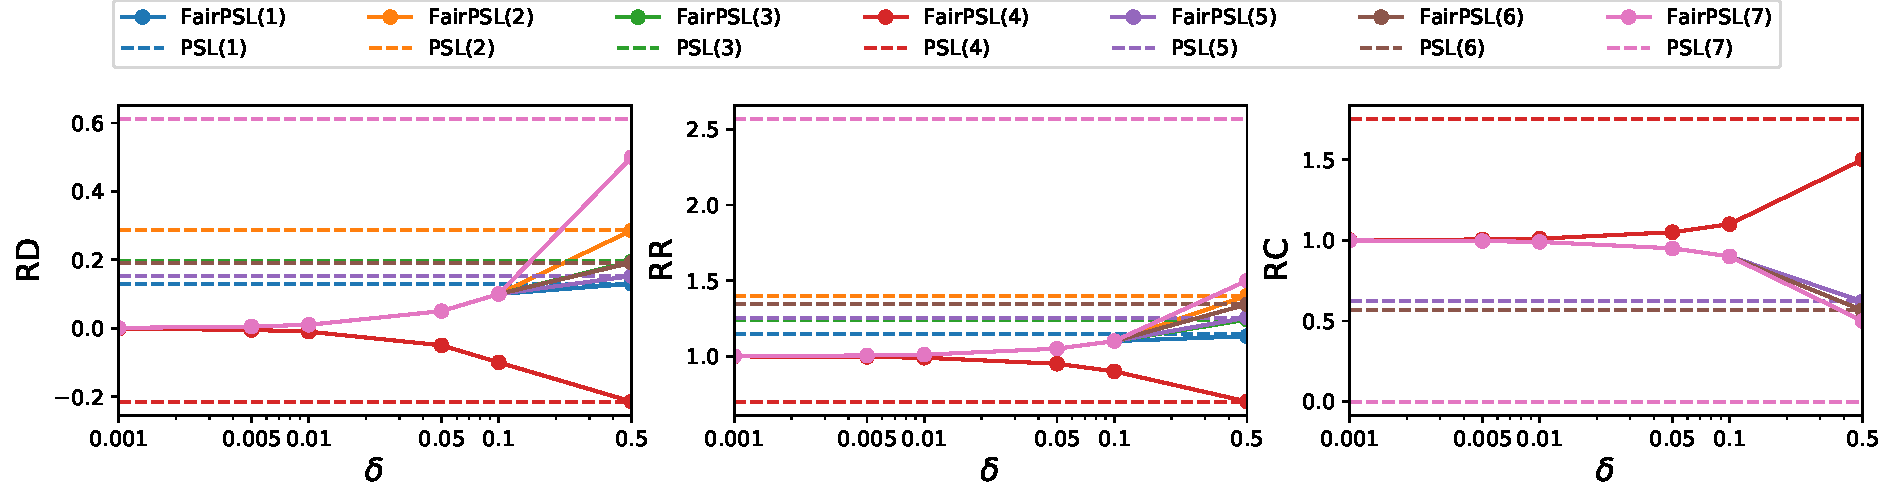
\includegraphics[width=1\linewidth]{figs/results_vis_uni_params.pdf}
\caption{\small Fairness score of predictions obtained by MAP inference of PSL and FairPSL, according to the fairness measures \emph{RD}, \emph{RR}, and \emph{RC}. The labels of datasets are mentioned with parenthesis next to the inference method. The FairPSL values of each measure are obtained by adding the $\delta$-fairness constraint of that measure.\label{fig:results}
}  
\end{figure}

To answer \textbf{Q1}, we run the MAP inference algorithm of PSL and FairPSL on seven synthetic datasets. 
We run the MAP inference of FairPSL multiple times on each dataset: For each of the three fairness measures, we add the corresponding $\delta$-fairness constraint with five thresholds $\{0.001, 0.005, 0.01, 0.05, 0.1, 0.5\}$.

Figure~\ref{fig:results} shows the fairness score of predictions in terms of the three fairness measures. As expected, tighter $\delta$-fairness constraints lead to better scores. Note that the best possible score according to RD is 0, as it computes a difference. Since RR and RC compute ratios, the best possible score according to these measures is 1. In our experiments, with any of these measures, taking $\delta = 0.001$ pushes the score of predictions to its limit.  

The $\delta$-fairness constraints modify the optimization problem of MAP inference by reducing the feasible region to solutions that conform with fairness guarantees. Research question \textbf{Q2} is concerned with the effect of this reduction on the accuracy of predictions. Note that decision quality is the same as the accuracy of predictions. To answer this question, we compare the inferred values for the decision atoms \textit{ToPromote(e)} against their actual values. These values are extracted from the known values of \textit{IsQualified(e)} according to rules 11 and 12 in Table~\ref{tab:pslmodel}. Figure~\ref{fig:accuracy} shows the area under the curve of the receiver operating characteristic~(AUC) of predicting the decision variable in three groups, namely the protected group, the unprotected group (i.e., promotion of the employees who have in-group managers), and all employees. By doing so, we make sure that our fairness constraints do not propagate bias towards either of the populations. Since the results of FairPSL with $\delta$-fairness constraints RR and RC are very similar to the results of RD, we only report the latter here.


\begin{figure}
    \centering
    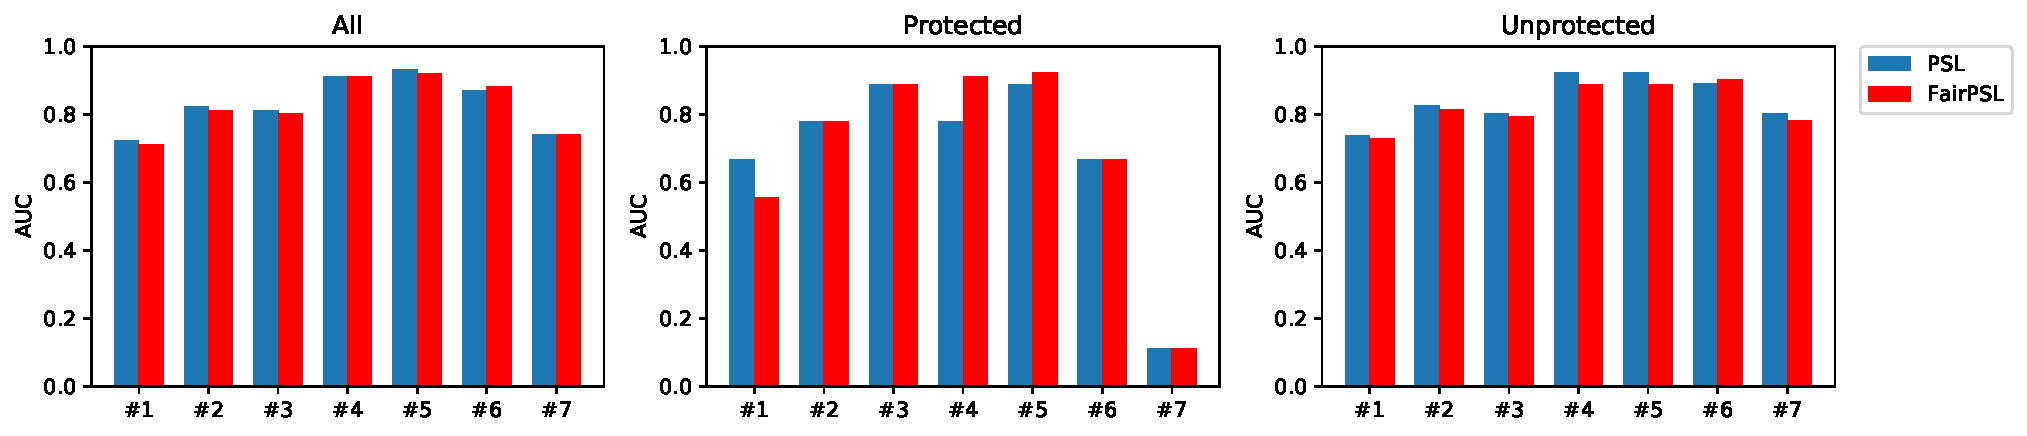
\includegraphics[width=\textwidth]{figs/roc.pdf}
    \caption{\small AUC score of predictions for truth values of unknown atoms \textit{ToPromote(e)} using MAP inference of PSL and FairPSL with $\delta$-fairness constraints $RD$ with $\delta=0.001$.}
    \label{fig:accuracy}
\end{figure}

According to Figure~\ref{fig:accuracy}, the results of both PSL and FairPSL in all seven datasets are close to each other. Note that although fairness may impose a cost in terms of overall accuracy, FairPSL often improves the accuracy of the protected class. Sometimes the overall predictions of FairPSL are even slightly better than PSL (e.g., dataset 6 and 7). As expected, the accuracy of the fourth setting where the opinions are unbiased are similar in both PSL and FairPSL. We observe that prediction of MAP inference for both FairPSL and PSL are similar, thus, in these settings at least, FairPSL guarantees fairness without hurting accuracy. Further investigation is required on the effect of the various ranges of discrimination (i.e., $\theta_1$, $\theta_2$, $\theta_3$, $\theta_4$) on the prediction results of FairPSL.



We also generate various types of organizations in which labels are not uniformly distributed, e.g., one population only occurs at the bottom levels of an organization. While we did not observe any differences in the behavior of our method with respect to accuracy and fairness measure, we found that the degree of discrimination is higher in such organizations. Further investigations on the structure of an organization on discrimination is an interesting direction for future research. 

\section{Conclusion and Future Directions}
\label{sec:conclusion}
Many applications of AI and machine learning affect peoples' lives in important ways. While there is a growing body of work on fairness in AI and ML, it assumes an individualistic notion of fairness.   In this paper, we have proposed a general framework for relational fairness which includes both a rich language for defining discrimination patterns and an efficient algorithm for performing inference subject to fairness constraints. We show our approach enforces fairness guarantees while preserving the accuracy of the predictions. 

There are many avenues for expanding on this work. For example, here we assumed that the discriminative pattern is given, however an automatic mechanism to extract discriminatory situations hidden in a large amount of decision records is an important and required task. Discrimination discovery has been studied for attribute-based fairness~\cite{pedreschi2013discovery}. An interesting next step is discrimination pattern discovery in relational data.

\section*{Acknowledgements}
This work is supported by the National Science Foundation under Grant Numbers CCF-1740850 and IIS-1703331. Golnoosh Farnadi and Behrouz Babaki are  supported by postdoctoral scholarships from IVADO through the Canada First Research Excellence Fund (CFREF) grant.

\begin{thebibliography}{10}
\itemsep=1pt 
\begin{small}

\bibitem{EUlaw}
European union legislation. (a) racial equality directive, 2000; (b) employment
  equality directive, 2000; (c) gender employment directive, 2006; (d) equal
  treatment directive (proposal), 2008.

\bibitem{UKlaw}
{UK} legislation. (a) sex discrimination act, 1975, (b) race relation act,
  1976.

\bibitem{USlaw}
United nations legislation. (a) universal declaration of human rights, 1948,
  (c) convention on the elimination of all forms of racial discrimination,
  1966, (d) convention on the elimination of all forms of discrimination
  against women, 1979.

\bibitem{alshukaili:iswc16}
Duhai Alshukaili, Alvaro A.~A. Fernandes, and Norman~W. Paton.
\newblock Structuring linked data search results using probabilistic soft
  logic.
\newblock In {\em International Semantic Web Conference {(1)}}, volume 9981 of
  {\em Lecture Notes in Computer Science}, pages 3--19, 2016.

\bibitem{bach:jmlr17}
Stephen~H. Bach, Matthias Broecheler, Bert Huang, and Lise Getoor.
\newblock Hinge-loss markov random fields and probabilistic soft logic.
\newblock {\em Journal of Machine Learning Research}, 18:109:1--109:67, 2017.

\bibitem{barocas2016big2}
Solon Barocas and Andrew~D Selbst.
\newblock Big data's disparate impact.
\newblock {\em California Law Review}, 104:671, 2016.

\bibitem{boyd2014networked}
Danah Boyd, Karen Levy, and Alice Marwick.
\newblock The networked nature of algorithmic discrimination.
\newblock In {\em Data and discrimination: Collected essays}, pages 53--57.
  2014.

\bibitem{brewer1979group}
Marilynn~B Brewer.
\newblock In-group bias in the minimal intergroup situation: A
  cognitive-motivational analysis.
\newblock {\em Psychological bulletin}, 86(2):307, 1979.

\bibitem{brewer2007social}
Marilynn~B Brewer.
\newblock The social psychology of intergroup relations: Social categorization,
  ingroup bias, and outgroup prejudice.
\newblock {\em Social Psychology: Handbook of Basic Principles}, 2007.

\bibitem{chouldechova2017fair2}
Alexandra Chouldechova.
\newblock Fair prediction with disparate impact: {A} study of bias in
  recidivism prediction instruments.
\newblock {\em CoRR}, abs/1703.00056, 2017.

\bibitem{dwork2012fairness3}
Cynthia Dwork, Moritz Hardt, Toniann Pitassi, Omer Reingold, and Richard~S.
  Zemel.
\newblock Fairness through awareness.
\newblock In {\em {ITCS}}, pages 214--226. {ACM}, 2012.

\bibitem{ebrahimi:emnlp16}
Javid Ebrahimi, Dejing Dou, and Daniel Lowd.
\newblock Weakly supervised tweet stance classification by relational
  bootstrapping.
\newblock In {\em {EMNLP}}, pages 1012--1017. The Association for Computational
  Linguistics, 2016.

\bibitem{farnadi2018fairness}
Golnoosh Farnadi, Behrouz Babaki, and Lise Getoor.
\newblock Fairness in relational domains.
\newblock In {\em AAAI/ACM Conference on AI, Ethics, and Society (AIES)}, pages
  108--114. ACM, 2018.

\bibitem{feldman2015certifying2}
Michael Feldman, Sorelle~A. Friedler, John Moeller, Carlos Scheidegger, and
  Suresh Venkatasubramanian.
\newblock Certifying and removing disparate impact.
\newblock In {\em {KDD}}, pages 259--268. {ACM}, 2015.

\bibitem{getoor2007introduction}
Lise Getoor and Ben Taskar.
\newblock {\em {Introduction to Statistical Relational Learning}}.
\newblock MIT press Cambridge, 2007.

\bibitem{hardt2016equality3}
Moritz Hardt, Eric Price, and Nati Srebro.
\newblock Equality of opportunity in supervised learning.
\newblock In {\em {NIPS}}, pages 3315--3323, 2016.

\bibitem{kamishima2011fairness}
Toshihiro Kamishima, Shotaro Akaho, and Jun Sakuma.
\newblock Fairness-aware learning through regularization approach.
\newblock In {\em ICDMW}, pages 643--650. {IEEE} Computer Society, 2011.

\bibitem{kouki:recsys15}
Pigi Kouki, Shobeir Fakhraei, James~R. Foulds, Magdalini Eirinaki, and Lise
  Getoor.
\newblock Hyper: {A} flexible and extensible probabilistic framework for hybrid
  recommender systems.
\newblock In {\em RecSys}, pages 99--106. {ACM}, 2015.

\bibitem{counterfactualfairness}
Matt~J. Kusner, Joshua~R. Loftus, Chris Russell, and Ricardo Silva.
\newblock Counterfactual fairness.
\newblock In {\em {NIPS}}, pages 4069--4079, 2017.

\bibitem{Pedreschi:2012}
Dino Pedreschi, Salvatore Ruggieri, and Franco Turini.
\newblock A study of top-k measures for discrimination discovery.
\newblock In {\em {SAC}}, pages 126--131. {ACM}, 2012.

\bibitem{pedreschi2013discovery}
Dino Pedreschi, Salvatore Ruggieri, and Franco Turini.
\newblock The discovery of discrimination.
\newblock In {\em Discrimination and Privacy in the Information Society},
  volume~3 of {\em Studies in Applied Philosophy, Epistemology and Rational
  Ethics}, pages 91--108. Springer, 2013.

\bibitem{ridgeway2004unpacking}
Cecilia~L Ridgeway and Shelley~J Correll.
\newblock Unpacking the gender system: A theoretical perspective on gender
  beliefs and social relations.
\newblock {\em Gender \& society}, 18(4):510--531, 2004.

\bibitem{sridhar:bioinformatics16}
Dhanya Sridhar, Shobeir Fakhraei, and Lise Getoor.
\newblock A probabilistic approach for collective similarity-based drug-drug
  interaction prediction.
\newblock {\em Bioinformatics}, 32(20):3175--3182, 2016.

\bibitem{verma2018fairness2}
Sahil Verma and Julia Rubin.
\newblock Fairness definitions explained.
\newblock In {\em 2018 IEEE/ACM International Workshop on Software Fairness
  (FairWare)}, pages 1--7. IEEE, 2018.

\bibitem{west2014exploiting}
Robert West, Hristo~S. Paskov, Jure Leskovec, and Christopher Potts.
\newblock Exploiting social network structure for person-to-person sentiment
  analysis.
\newblock {\em {TACL}}, 2:297--310, 2014.

\bibitem{zafar2017parity}
Muhammad~Bilal Zafar, Isabel Valera, Manuel Gomez{-}Rodriguez, Krishna~P.
  Gummadi, and Adrian Weller.
\newblock From parity to preference-based notions of fairness in
  classification.
\newblock In {\em {NIPS}}, pages 228--238, 2017.

\bibitem{zemel2013learning}
Richard~S. Zemel, Yu~Wu, Kevin Swersky, Toniann Pitassi, and Cynthia Dwork.
\newblock Learning fair representations.
\newblock In {\em {ICML} {(3)}}, volume~28 of {\em {JMLR} Workshop and
  Conference Proceedings}, pages 325--333. JMLR.org, 2013.

\end{small}
\end{thebibliography}

\end{document}

\end{article}

\begin{article}
{XuanYuan: An AI-Native Database}
{Guoliang Li, Xuanhe Zhou, Sihao Li}
\graphicspath{{submissions/ainative/}}
%\documentclass[11pt,dvipdfm]{article}
\documentclass[11pt]{article}
\usepackage{deauthor,times,graphicx} %required
\usepackage{amsmath,amssymb}
\usepackage{multirow}
\usepackage{algorithm}
\usepackage{algpseudocode}
\usepackage{todonotes}
\usepackage{url}

% \graphicspath{{farnadi/}}

\newtheorem{mydef}{\textbf{Definition}}
\newtheorem{myex}{\textbf{Example}}
\newtheorem{mytheorem}{\textbf{Theorem}}


\begin{document}

\title{A Declarative Approach to Fairness in Relational Domains}
\author{Golnoosh Farnadi$^{1,2}$, Behrouz Babaki$^1$, Lise Getoor$^3$\\
$^1$Polytechnique Montr\'{e}al, $^2$ Mila, $^3$ UC Santa Cruz \\
farnadig@mila.quebec, behrouz.babaki@polymtl.ca, getoor@soe.ucsc.edu}

\maketitle

\begin{abstract}
AI and machine learning tools are being used with increasing frequency for decision making in domains that affect peoples' lives such as employment, education, policing and %loan approval
financial qualifications. These uses raise concerns about biases of algorithmic discrimination and have motivated the development of fairness-aware machine learning. However, existing fairness approaches are based solely on attributes of individuals. In many cases, discrimination is much more complex, and taking into account the social, organizational, and other connections between individuals is important. We introduce new notions of fairness that are able to capture the relational structure in a domain. We use first-order logic to provide a flexible and expressive language for specifying complex relational patterns of discrimination. Furthermore, we extend an existing statistical relational learning framework, probabilistic soft logic~(PSL), to incorporate our definition of relational fairness. We refer to this fairness-aware framework FairPSL. FairPSL makes use of the logical definitions of fairnesss but also supports a probabilistic interpretation. In particular, we show how to perform maximum a posteriori~(MAP) inference by exploiting probabilistic dependencies within the domain while avoiding violations of fairness guarantees. Preliminary empirical evaluation shows that we are able to make both accurate and fair decisions.
\end{abstract}

\section{Introduction}
\label{sec:introduction}

Over the past few years, AI and machine learning have become essential components in operations that drive the modern society, e.g., in financial, administrative, and educational spheres. \emph{Discrimination} happens when qualities of individuals which are not relevant to the decision making process influence the decision. Delegating decision making to an automated process raises questions about discriminating against individuals with certain traits based on biases in the data. This is especially important when the decisions have the potential to impact the lives of individuals, for example, the decisions on granting loans, assigning credit, and employment. 

\emph{Fairness} is defined as the absence of discrimination in a decision making process. The goal of \emph{fairness-aware} machine learning is to ensure that the decisions made by an algorithm do not discriminate against a population of individuals~\cite{feldman2015certifying2,boyd2014networked,hardt2016equality3}. Fairness has been well studied in the social sciences and legal scholarship (for an in-depth review see~\cite{barocas2016big2}), and there is emerging work on fairness-aware ML within the AI and computer science communities. For example, fairness through awareness/Lipschitz property~\cite{dwork2012fairness3}, individual fairness~\cite{zemel2013learning}, statistical parity/group fairness~\cite{kamishima2011fairness}, counterfactual fairness~\cite{counterfactualfairness}, demographic parity/disparate impact~\cite{feldman2015certifying2,chouldechova2017fair2}, preference-based fairness~\cite{zafar2017parity}, and equality of opportunity~\cite{hardt2016equality3}.

The existing work in fairness-aware machine learning is based on a definition of discrimination where a decision is influenced by an \emph{attribute} of an individual. An attribute value upon which discrimination is based (such as gender, race, or religion) is called a \emph{sensitive attribute}. The sensitive attribute defines a population of vulnerable individuals known as the \emph{protected group}. A fair decision-making process treats the protected group the same as the \emph{unprotected group}. 

However, in many social contexts, discrimination is the result of complex interactions and can not be described solely in terms of attributes of an individual. For example, consider an imaginary scenario in an organization in which younger female workers who have older male supervisors have lower chances of promotion than their male counterparts.\footnote{Of course, many other patterns may be possible: female bosses may promote female subordinates and discriminate against male workers, or male bosses may promote female employees.  Our goal is to provide a general framework which is able to describe arbitrarily complex discrimination patterns.} 
 This discrimination pattern involves two attributes of the individual (gender and age), a relationship with another individual (supervisor), and two attributes of the second individual. Addressing such complex cases poses two challenges. First, the concepts of discrimination and fairness need to be extended to capture not only attributes of individuals but also the relationships between them. Second, a process is required that ensures that fair decisions are made about individuals who are affected by such patterns. In this paper we address both of these challenges.
We use first-order logic (FOL) to extend the notion of fairness to the relational setting. FOL is an expressive representation for relational problems which is also widely used for learning in relational domains. Moreover, we extend an existing framework for statistical relational learning~\cite{getoor2007introduction} called probabilistic soft logic (PSL)\footnote{http://psl.linqs.org/}~\cite{bach:jmlr17}. PSL combines logic and probability for learning and reasoning over uncertain relational domains. One of the most common reasoning tasks in PSL is called maximum a posteriori (MAP) inference, which is performed by finding the most probable truth values for unknowns over a set of given evidence. We develop a new MAP inference algorithm which is able to maximize the a posteriori values of unknown variables \emph{subject to} fairness guarantees. An early version of this paper which this work builds upon and extends appeared in~\cite{farnadi2018fairness}.

\looseness-1
Our contributions are as follows: 1) we propose fairness-aware machine learning for the relational setting; 2) we extend PSL into a fairness-aware framework called FairPSL which can represent the logical definition of fairness; 3) we develop a new MAP inference algorithm which is able to maximize the posteriori values of unknown variables \emph{subject to} fairness guarantees; 4) we empirically evaluate our proposed framework on synthetic data. 

\section{Motivation}
\label{sec:motivation}

Discrimination in social contexts have been studied in the field of social psychology~\cite{brewer2007social,brewer1979group,ridgeway2004unpacking}. There is a large literature on various aspects of relational bias in social contexts such as \emph{in-group-out-group bias}, \emph{gender bias}, and \emph{ethnicity-based favoritism} that can result in discrimination. 
As an example, consider gender bias in the workplace that reflects stereotypically masculine criteria and male-based favoritism. Such gender bias 
typically places women in lower positions and negatively impacts their opportunities. Further, lack of women in leadership positions may affect the promotion of women and results in a glass ceiling that keeps women from rising beyond a certain level in the hierarchy. This scenario shows that considering  protected attributes such as gender is not always sufficient to detect the source of bias and avoid discrimination, one also has to consider the relational information, in this case the organization hierarchy. Note that this can be generalized to any ingroup/outgroup scenario where the sensitive attribute could be race, religion, age, marital-status, etc.

The existing work on designing fair algorithms in machine learning exclusively focuses on \emph{attribute-based fairness}, which is based on the following assumptions: First, there is an assumption that the individuals (sometimes referred to as units or entities) are independent and described by simple attribute vectors. Second, the group for which one wishes to ensure fairness (known as the \emph{protected group}) is defined on the basis of some attribute values. Finally, there is a decision that is associated with each individual, and the goal is to ensure that members of the protected group are subject to a fair decision (we discuss different fairness measures in Section~\ref{sec:fairnessmeasure}).  We illustrate  attribute-based fairness in the following example. 

\begin{myex}[Loan Processing]
\label{ex:loan}
A bank bases its decisions about granting a loan on attributes of the applicant. The goal is to decide whether to grant a loan to an applicant using a predictive model. The bank needs to ensure that the obey fair lending practices and ensure that gender, race, sexual orientation of applicants has no influence on the decision. In this scenario, the protected group is the historically disadvantaged applicants.  
\end{myex}
The current fairness-aware machine learning techniques are not capable of modeling relations and hence cannot be used to make the decision making model fair. However, in many decision making scenarios, especially in social and organizational settings, the domain is relational, and the protected group itself might be best represented using a relational definition. We illustrate this setting in the following scenario:
\begin{myex}[Performance Review]
\label{ex:review}
Consider an organization where decisions about the promotion of employees is based on two criteria: 1) an objective performance measure, and 2) the opinion of their direct and indirect managers above them. The opinions are inferred from the performance reviews which are collected periodically. Not every manager can submit a review for all its subordinates, this is especially the case for top-level managers who have a large number of subordinates. Hence, the opinions of managers are collectively inferred from the opinions of their sub-ordinates. However, some employees may be biased, and judge other employees unfavorably, by favoring employees who are similar to themselves (same gender, race, religion, etc.) over employees who are dissimilar. The organization needs to ensure that promotion of employees do not have any relational bias caused by in-group-out-group favoritism.

\end{myex}
Example~\ref{ex:review} describes a prediction problem over a database that consists of relations between employees. Such prediction tasks are best handled by techniques from the relational learning domain. To ensure fair prediction in such settings, we need to extend the notion of \emph{attribute-based fairness} to \emph{relational fairness}. Throughout this paper, we use the performance review problem as a running example for relational fairness.

\section{Fairness Formalism}
\label{sec:formulation}

A representation that can describe different types of entities and different relationships between them is called relational. In this section, we use first-order logic to define relational fairness. We employ first-order logic as an expressive representation formalism which can represent objects and complex relationships between them. We start by defining an atom:

\begin{mydef}[Atom]
An atom is an expression of the form $P(a_1, a_2, \ldots, a_n)$ where each argument $a_1, a_2,$ $\ldots,$ $a_n$ is either a constant or a variable. The finite set of all possible substitutions of a variable to a constant for a particular variable $a$ is called its \textit{domain} $D_{a}$. If all variables in $P(a_1, a_2, \ldots, a_n)$ are substituted by some constant from their respective domain, then we call the resulting atom a \textit{ground atom}. 
\end{mydef}

\begin{myex}
In our loan processing problem (Example~\ref{ex:loan}), we can represent applicants' attributes by atoms. For instance, atom $Female(v)$ indicates whether or not applicant $v$ is female. Similarly, we can represent relations with atoms. In the performance review problem in Example~\ref{ex:review} the atom $Manager(m,e)$ indicates whether or not employee $m$ is a direct or indirect manager of employee $e$.
\end{myex}

The relational setting provides the flexibility to express complex definitions with formulae.

\begin{mydef}[Formula] 
A formula is defined by induction: every atom is a formula. If $\alpha$ and $\beta$ are formulae, then $\alpha \vee \beta$, $\alpha \wedge \beta$, $\neg \alpha$, $\alpha \rightarrow \beta$ are formulae. If $x$ is a variable and $\alpha$ is a formula, then the quantified expressions of the form $\exists x$ $\alpha$ and $\forall x$ $\alpha$ are formulae.    
\end{mydef}

To characterize groups of individuals based on a formula, we define the notion of \emph{population}.

\begin{mydef}[Population]
We denote formula $F$ which has only one free variable $v$ (i.e., other variables in $F$ are quantified) by $F[v]$. The population defined by $F[v]$ is the set of substitutions of $v$ for which $F[v]$ holds.   
\end{mydef}


\begin{myex}
\label{ex:disformula}
Consider the formula $F[v] := \forall u, \, \textit{Manager}(u,v) \rightarrow \neg \textit{SameGroup}(u, v)$. The population specified by this formula is the set of individuals all of whose managers belong to a group different from theirs. 
\end{myex}

The truth value of a formula is derived from the truth value of atoms that it comprises, according to the rules of logic. Each possible assignment of truth values to ground atoms is called an \emph{interpretation}. 


\begin{mydef}[Interpretation]
An interpretation $I$ is a mapping that associates a truth value $I(P)$ to each ground atom $P$. For Boolean truth values, $I$ associates true to 1 and false to 0 truth values. For soft logic (see Definition~\ref{def:softlogic}) $I$ maps each ground atom $P$ to a truth value in interval $[0, 1]$.
\end{mydef}

In attribute-based fairness, it is assumed that there is a certain attribute of individuals, i.e, the sensitive attribute,  that we do not want to affect a decision. Gender, race, religion and marital status are examples of sensitive attributes. Discrimination has been defined in social science studies as a treatment in favor or against a group of individuals given their sensitive attribute. This group of individuals is the protected group. 

In a relational setting, both the sensitive attributes of an individual and their participation in various relations may have an undesired effect on the final decision. We characterize the protected group in a relational setting by means of a population. In practice, we are often interested in maintaining fairness for a specific population such as applicants, students, employees, etc. This population is then partitioned into the protected and unprotected groups. We define a \emph{discriminative pattern} which is a pair of formulae to capture these groups: 1) $F_1[v]$: to specify the difference between the protected and unprotected groups and 2) $F_2[v]$: to specify the population over which we want to maintain fairness. 

\begin{mydef}[Discriminative pattern]
A discriminative pattern is a pair $\textit{DP}[v]:=(F_1[v], F_2[v])$ , where $F_1[v]$ and $F_2[v]$ are formulae.
\end{mydef}

\begin{myex}
\label{ex:pattern}
The two formulae in the discrimination pattern $\textit{DP}[v]:= \big((\forall u, \,  \textit{Manager}(u,v) \rightarrow  \neg \textit{SameGroup}(u, v)),$ $\textit{Employee}(v)\big)$ specify two populations, namely all employees and those employees who belong to a group different from their managers.
\end{myex}

Given the definition of the discriminative pattern, we have a rich language to define the scope of the protected and unprotected groups in a relational setting.

\begin{mydef}[Protected group] Given an interpretation $I$, the protected group is a population of the form:
{$$PG :=\{ v : F_1[v] \wedge F_2[v]\}$$}
which is defined as the set of all instances hold for variable $v$ for which $F_1[v] \wedge F_2[v]$ is true under interpretation $I$, that is, $I(F_1[v] \wedge F_2[v]) = 1$. 
Similarly, the \emph{unprotected group} is a population of the form: 
{$$UG := \{ v : \neg F_1[v] \wedge  F_2[v]\}$$}
which is defined as the set of all instances hold for variable $v$ 
for which $I(\neg F_1[v] \wedge F_2[v]) = 1$. 
\end{mydef}

\begin{myex}
The protected group of the discrimination pattern specified in Example~\ref{ex:pattern} is {$PG := \big\{ v : \big(\forall u, \,$ $ \textit{Manager}(u, v) \rightarrow \neg \textit{SameGroup}(u, v)\big) \wedge \textit{Employee}(v) \big\}$} and the unprotected group is {$UG :=  \big\{ v:  \big(\exists u, \, \textit{Manager}(u,v) \wedge \textit{SameGroup}(u, v)\big) \wedge \textit{Employee}(v) \big\}$}. This means our protected group is the set of employees belonging to a group different from their managers,
and our unprotected group consists of other employees. 
\end{myex}

Discrimination is defined in terms of a treatment or decision that distinguishes between the protected and unprotected groups. Here we define the \emph{decision} atom.
\begin{mydef}[Decision atom] A decision atom $d(v)$ is an atom containing exactly one variable $v$ that specifies a decision affecting the protected group which is defined either by law or end-user.
\end{mydef}
\begin{myex}
The decision atom ${\textit ToPromote}(v)$ indicates whether or not $v$ receives a promotion.
\end{myex}

Note that the fairness formulation in this section is designed for the relational setting, however relational fairness subsumes the attribute-based fairness such that: a sensitive attribute is defined by an atom with one argument and $F_2[v]$ in discrimination pattern is $\textit{Applicant}(v)$. For example, discrimination pattern of our loan processing problem in Example~\ref{ex:loan} is of the form $\textit{DP} := ( \textit{Female}(v), \textit{Applicant}(v))$ that denotes female applicants as the protected group (i.e., $PG :=  \{ v: \textit{Female}(v) \}$) and male applicants as the unprotected group (i.e., $UG := \{ v: \neg \textit{Female}(v)\}$).


\section{Fairness Measures}
\label{sec:fairnessmeasure}

Over the past few years, many fairness measures have been introduced~\cite{verma2018fairness2}. An important class of these measures are \emph{group fairness} measures which quantify the inequality between different subgroups. Some of the most popular measures in this class include \emph{equal opportunity}, \emph{equalized odds}, and \emph{demographic parity}~\cite{hardt2016equality3}. In this paper we restrict our focus to the latter. In an attribute-value setting, demographic parity means that the decision should be independent of the protected attributes. Assume that binary variables $A$ and $C$ denote the decision and protected attributes, and the preferred value of $A$ is one. Demographic parity requires that:

\begin{equation*}
    P(A=1 | C=0) = P(A=1 | C=1)
\end{equation*}

We will now generalize this measure to the relational setting using the notations defined in Section~\ref{sec:formulation}. Let $a$ and $c$ denote the counts of denial (i.e., negative decisions) for protected and unprotected groups, and $n_{1}$ and $n_{2}$ denote their sizes, respectively. Given the decision atom $d(v)$, discriminative pattern $\textit{DP}(F_1[v], F_2[v])$, and interpretation $I$, these counts are computed by the following equations: 
{
\begin{flalign}
    & a \equiv \sum_{v \in D_v} I\big( \neg d(v) \wedge  F_1[v] \wedge F_2[v]) \label{eq:a}\\
    & c \equiv \sum_{v \in D_v} I\big( \neg d(v) \wedge  \neg F_1[v] \wedge  F_2[v]) \label{eq:c}\\
    & n_{1} \equiv \sum_{v \in D_v} I\big(F_1[v] \wedge F_2[v]) \label{eq:n1}\\
    & n_{2} \equiv \sum_{v \in D_v} I\big(\neg F_1[v] \wedge  F_2[v]) \label{eq:n2}
\end{flalign}}
The proportions of denying for protected and unprotected groups are $p_1 = \frac{a}{n_1}$ and $p_2 = \frac{c}{n_2}$, respectively. There are a number of data-driven measures~\cite{Pedreschi:2012} which quantify demographic disparity and can be defined in terms of $p_1$ and $p_2$:
\begin{itemize}
    \item \textbf{Risk difference}: $RD = p_1 - p_2$, also known as absolute risk reduction. 
    \item \textbf{Risk Ratio}: $RR = \frac{p_1}{p_2}$, also known as relative risk. 
    \item \textbf{Relative Chance}: $RC = \frac{1 - p_1}{1 - p_2}$ also, known as selection rate.
\end{itemize}
These measures have been used in the legal systems of European Union, UK, and US~\cite{EUlaw,UKlaw,USlaw}. Notice that RR is the ratio of the proportion of benefit denial between the protected and unprotected groups, while RC is the ratio of the proportion of benefit granted. Finally, we introduce the notion of $\delta$-fairness.

\begin{mydef}[$\delta$-fairness]
If a fairness measure for a decision making process falls within some $\delta$-window, then the process is \emph{$\delta\text{-fair}$}. Given $0 \leq \delta \leq 1$, the  $\delta$-windows for measures RD/RR/RC are defined as:
{\begin{flalign*}
	     - \delta \leq &RD \leq \delta \\
	     1- \delta \leq &RR \leq 1+ \delta\\
	     1- \delta \leq &RC \leq 1+ \delta
	\end{flalign*}}
\end{mydef}

To overcome the limitations of attribute-based fairness, we introduce a new statistical relational learning~(SRL) framework~\cite{getoor2007introduction} suitable for modelling fairness in relational domain. In the next section, we review probabilistic soft logic~(PSL). We then extend PSL with the definition of relational fairness introduced above in Section~\ref{sec:fairMAP}. Our fairness-aware framework, ``FairPSL'', is the first SRL framework that performs fair inference. 

\section{Background: Probabilistic Soft Logic}
\label{sec:psl}

In this section, we review the syntax and semantics of PSL, and in the next section we extend MAP inference in PSL with fairness constraints to define MAP inference in FairPSL.

PSL is a probabilistic programming language for defining hinge-loss Markov random fields~\cite{bach:jmlr17}. Unlike other SRL frameworks whose atoms are Boolean, atoms in PSL can take continuous values in the interval $[0,1]$. PSL is an expressive modeling language that can incorporate domain knowledge with first-order logical rules and has been used successfully in various domains, including bioinformatics~\cite{sridhar:bioinformatics16}, recommender systems~\cite{kouki:recsys15}, natural language processing~\cite{ebrahimi:emnlp16}, information retrieval~\cite{alshukaili:iswc16}, and social network analysis~\cite{west2014exploiting}, among many others. 
 
A PSL model is defined by a set of first-order logical rules called \emph{PSL rules}.

\begin{mydef} [PSL rule] a PSL rule $r$ is an expression of the form:
{\begin{equation}
\lambda_{r}: T_1 \land T_2 \land \ldots \land T_w \rightarrow H_1 \vee H_2 \vee \ldots \vee H_l
\end{equation}}

where { $T_1, T_2, \ldots, T_w, H_1, H_2, \ldots, H_l$} are atoms or negated atoms and { $\lambda_{r} \in \mathbb{R}^{+} \cup \infty$} is the weight of the rule $r$.  We call { $T_1 \land T_2 \land \ldots \land T_w$} the body of $r$ ($r_{body}$), and { $H_1 \vee H_2 \vee \ldots \vee H_l$} the head of $r$ ($r_{head}$).
\end{mydef}


Since atoms in PSL take on continuous values in the unit interval $[0,1]$, next we define soft logic to calculate the value of the PSL rules under an interpretation $I$.

\begin{mydef}[Soft logic]
\label{def:softlogic}
The ({$\tilde{\wedge}$}) and ({$\tilde{\vee}$}) and negation ({$\tilde{\neg}$}) are defined as follows. For {$m, n \in [0,1]$} we have: {$m \tilde{\wedge} n = \max(m+n -1, 0)$}, {$m \tilde{\vee} n = \min(m+n , 1)$} and {$\tilde{\neg} m = 1 - m$}. The $\, \tilde{} \,$ indicates the relaxation over Boolean values.
\end{mydef}

The probability of truth value assignments in PSL is determined by the rules' \emph{distance to satisfaction}.

\begin{mydef}[The distance to satisfaction]
The distance to satisfaction $d_{r}(I)$ of a rule $r$ under an interpretation $I$ is defined as:
{
\begin{equation}
d_{r}(I) = \max\{0, I(r_{body})-I(r_{head})\}
\end{equation}}
\end{mydef}

By using Definition~\ref{def:softlogic}, one can show that the closer the interpretation of a grounded rule $r$ is to 1, the smaller its distance to satisfaction. A PSL model induces a distribution over interpretations $I$. Let $R$ be the set of all grounded rules, then the probability density function is:
{
\begin{equation}
f(I) ={\frac{1}{Z}} \exp[-\sum_{r\in R} \lambda_{r}(d_{r}(I))^p]
\label{eq:potential}
\end{equation}
}
\noindent where { $\lambda_{r}$} is the weight of rule $r$, {
$Z = \int_{I} \exp[ -\sum_{r\in R} \lambda_{r}(d_{r}(I))^p]$
} is a normalization constant, and { $p \in \{1,2\}$} provides a choice of two different loss functions, $p=1$ (i.e., linear), and $p=2$ (i.e, quadratic). These probabilistic models are instances of hinge-loss Markov random fields~(HL-MRF)~\cite{bach:jmlr17}. The goal of maximum a posteriori (MAP) inference is to find the most probable truth assignments $I_{\textit{MPE}}$ of unknown ground atoms given the evidence which is defined by the interpretation $I$. Let $X$ be all the evidence, i.e., $X$ is the set of ground atoms such that $\forall x \in X, I(x)$ is known, and let $Y$ be the set of ground atoms such that $\forall y \in Y, I(y)$ is unknown. Then we have
{
\begin{equation}
I_{\textit{MAP}}(Y) = \textit{arg}\max_{I(Y)} P(I(Y)|I(X))
\end{equation}}
Maximizing the density function in Equation~\ref{eq:potential} is equivalent to minimizing the weighted sum of the distances to satisfaction of all rules in PSL. 

\begin{table*}[t]
    \centering
    \begin{tabular}{|lll|}
    \hline
    &&\\
    $R1$ & $\lambda_1$ &: $\textit{IsQualified}(e) \rightarrow \textit{HighPerformance}(e)$ \\
    $R2$ & $\lambda_1$ &: $\neg \textit{IsQualified}(e) \rightarrow \neg \textit{HighPerformance}(e)$ \\
    $R3$ & $\infty$ &: $\textit{PositiveReview}(e1, e2) \rightarrow \textit{PositiveOpinion}(e1, e2)$ \\
    $R4$ & $\infty$ &: $\neg \textit{PositiveReview}(e1, e2) \rightarrow \neg \textit{PositiveOpinion}(e1, e2)$ \\
    $R5$ & $\lambda_1$ &: $\textit{PositiveOpinion}(e1, e2) \wedge \textit{Manager}(m, e1) \rightarrow \textit{PositiveOpinion}(m, e2)$ \\
    $R6$ & $\lambda_1$ &: $\neg \textit{PositiveOpinion}(e1, e2) \wedge \textit{Manager}(m, e1) \rightarrow \neg \textit{PositiveOpinion}(m, e2)$ \\
    $R7$ & $\lambda_1$ &: $\textit{PositiveOpinion}(m, e) \wedge \textit{Manager}(m, e) \rightarrow \textit{IsQualified}(e)$ \\
    $R8$ & $\lambda_1$ &: $\neg \textit{PositiveOpinion}(m, e) \wedge \textit{Manager}(m, e) \rightarrow \neg \textit{IsQualified}(e)$ \\
    $R9$ &  $\lambda_1$ &: $\neg \textit{ToPromote}(e)$\\
    $R10$ & $\infty$ &: $\textit{IsQualified}(e) \rightarrow \textit{ToPromote}(e)$ \\
    $R11$ & $\infty$ &: $\neg \textit{IsQualified}(e) \rightarrow \neg \textit{ToPromote}(e)$ \\
    &&\\
    \hline
    \end{tabular}
    \caption{\small A simplified PSL model for the \emph{Performance Reviewing} problem}
    \label{tab:pslmodel}
\end{table*}

\begin{myex}
\label{ex:pslmodel}
The simplified PSL model for the performance reviewing problem in Example\ref{ex:review} is given in Table~\ref{tab:pslmodel}. The goal of MAP inference for this problem is to infer employees to promote. We simplified the model by assigning the same weight to all soft rules (i.e., $\lambda_i= 1$ where $i=\{1,2,5,6,7,8,9\}$). Below we explain the meaning of each rule in the model.

Rule $R1$ indicates that qualified employees have high performance and similarly rule $R2$ expresses that a negative qualification of employees is derived from their low performance. Rules $R5$ and $R6$ presents the propagation of opinion from bottom to top of the organizational hierarchy, i.e., managers have similar opinions towards employees given the opinions of their sub-ordinate managers. And rules $R7$ and $R8$ indicate that the positive/negative opinion of direct/indirect managers derive from the qualification of an employee. Rule $R9$ indicates the prior that not all employees get promoted. We also have four hard constraints (i.e., rules $R3$, $R4$, $R10$ and $R11$) where the weight of the rules are $\infty$. Rules $R3$ and $R4$ indicate that submitted positive/negative reviews should reflect positive/negative opinions. And two rules $R10$ and $R11$ show that a highly qualified employee should get promoted. 
\end{myex}

\section{Fairness-aware PSL (FairPSL)}
\label{sec:fairMAP}

The standard MAP inference in PSL aims at finding values that maximize the conditional probability of unknowns. Once a decision is made according to these values, one can use the fairness measure to quantify the degree of discrimination. A simple way to incorporate fairness in MAP inference is to add the $\delta$-fairness constraints to the corresponding optimization problem.   

Consider risk difference, $\textit{RD}$, where $\textit{RD} \equiv \frac{\mathbf{a}}{n_1} - \frac{\mathbf{c}}{n_2}$. The $\delta$-fairness constraint $-\delta \leq \textit{RD} \leq \delta$ can be encoded as the following constraints:
{\begin{align}
    & n_2 \mathbf{a} - n_1 \mathbf{c} - n_1 n_2 \delta \leq 0 \label{eq:RD1}\\
    & n_2 \mathbf{a} - n_1 \mathbf{c} + n_1 n_2 \delta \geq 0
\end{align}}
Similarly, from $\textit{RR} \equiv \frac{\mathbf{a} / n_1}{\mathbf{c} / n_2}$ and the $\delta$-fairness constraint $1 - \delta \leq \textit{RR} \leq 1 + \delta$ we obtain:
{\begin{align}
    & n_2 \mathbf{a} - (1 + \delta) n_1 \mathbf{c} \leq 0 \\
    & n_2 \mathbf{a} - (1 - \delta) n_1 \mathbf{c} \geq 0
\end{align}}
And finally, $\textit{RC} \equiv \frac{1 - \mathbf{a} / n_1}{1 - \mathbf{c} / n_2}$ and the $\delta$-fairness constraint $1 - \delta \leq \textit{RC} \leq 1 + \delta$ gives:
{ \begin{align}
    & - n_2 \mathbf{a} + (1 + \delta) n_1 \mathbf{c} - \delta n_1 n_2 \leq 0 \\
    & - n_2 \mathbf{a} + (1 - \delta) n_1 \mathbf{c} + \delta n_1 n_2 \geq 0 \label{eq:RC2}
\end{align}}
A primary advantage of PSL over similar frameworks is that its MAP inference task reduces to a convex optimization problem which can be solved in polynomial time. To preserve this advantage, we need to ensure that the problem will remain convex after the addition of $\delta$-fairness constraints. 

\begin{mytheorem}
The following condition is sufficient for preserving the convexity of MAP inference problem after addition of $\delta$-fairness constraints: The formulae $F_1[v]$ and $F_2[v]$ do not contain an atom $y \in Y$ and all atoms in $F_1[v]$ and $F_2[v]$ have values zero or one.
\end{mytheorem}
\begin{proof}
Since $I(F_1[v])$ and $I(F_2[v])$ do not depend on $I(Y)$, the values $n_{1}$ and $n_{2}$ are constants that can be computed in advance. Let us define the sets $D_v^a = \{ v \in D_v : F_1[v] \wedge F_2[v] \, \text{is true} \}$ and $D_v^c = \{ v \in D_v : \neg F_1[v] \wedge F_2[v] \, \text{is true} \}$. Since $F_1[v]$ and $F_2[v]$ can be only zero or one, we can rewrite the equations~\ref{eq:a} and \ref{eq:c} as:
{
\begin{align*}
    & \mathbf{a} = \sum_{v \in D_v^a} I(\neg d(v)) = |D_v^a| - \sum_{v \in D_v^a} I(d(v))\\
    & \mathbf{c} = \sum_{v \in D_v^c} I(\neg d(v)) = |D_v^c| - \sum_{v \in D_v^c} I(d(v))
\end{align*}}
\noindent which indicates that $\mathbf{a}$ and $\mathbf{c}$ can be expressed as linear combinations of variables in the optimization problem. This means that constraints~\ref{eq:RD1}-\ref{eq:RC2} are linear. Hence, addition of these constraints preserves the convexity of the optimization problem. 
\end{proof}

\section{Experiments}
\label{sec:experiment}

\begin{figure}
  \begin{minipage}[c]{0.6\textwidth}
    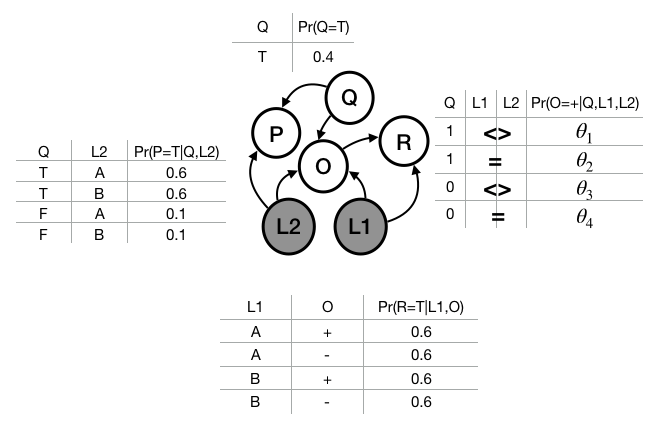
\includegraphics[width=\textwidth]{figs/BN.png}
  \end{minipage}\hfill
  \begin{minipage}[c]{0.45\textwidth}
    \caption{
        \small The model used for generating the datasets. There are four binary random variables, P, Q, O, and R. \textbf{P}: indicates whether or not the employee has high performance; \textbf{Q}: indicates whether or not an employee has high qualification; \textbf{O}: indicates whether or not the colleague submits the positive opinion towards the employee;  \textbf{R}: indicates whether or not the colleague has a positive opinion towards the employee;  \textbf{L1, L2}: indicates the label of the review provider and review receiver (observed).
    } \label{fig:BN}
  \end{minipage}
\end{figure}

We show the effectiveness of FairPSL by performing an empirical evaluation. We investigate two research questions in our experiments:
\begin{description}
\item[Q1] What is the effect of the fairness threshold $\delta$ on the fairness measures $RD/RC/RR$?
\item[Q2] How is decision quality affected by imposing $\delta$-fairness constraints?
\end{description}

Note that although we present the result for specific parameters of the framework in this section, we ran extensive analysis and the results we present are representative. We implemented the MAP inference routines of PSL and FairPSL in Python, using Gurobi-8.1\footnote{\url{www.gurobi.com}} as the backend solver. The FairPSL code, code for the data generator and data is publicly available\footnote{https://github.com/gfarnadi/FairPSL}. 

\subsection{Data generation}
  
We evaluate the FairPSL inference algorithm on synthetic datasets representing the performance review scenario (introduced in Example~\ref{ex:review}). The organization hierarchy is generated synthetically. 
The organization hierarchy generator is parameterized by two numbers: the number of employees in the organization ($n$) and the number of employees managed by each manager ($k$). Each employee is randomly assigned with a label \emph{A} or \emph{B}. An examples organization hierarchy with $n$=50 and $k$=3 is shown in Figure~\ref{fig:hierachy}.

\begin{figure}
  \begin{minipage}[c]{0.3\textwidth}
    \caption{
        \small An example of an organizational hierarchy with five levels and 50 employees with k=3. Each employee either has label A (shown with grey) or B (shown with white).
    }\label{fig:hierachy} 
	\end{minipage} \hfill
    \begin{minipage}[c]{0.7\textwidth}
    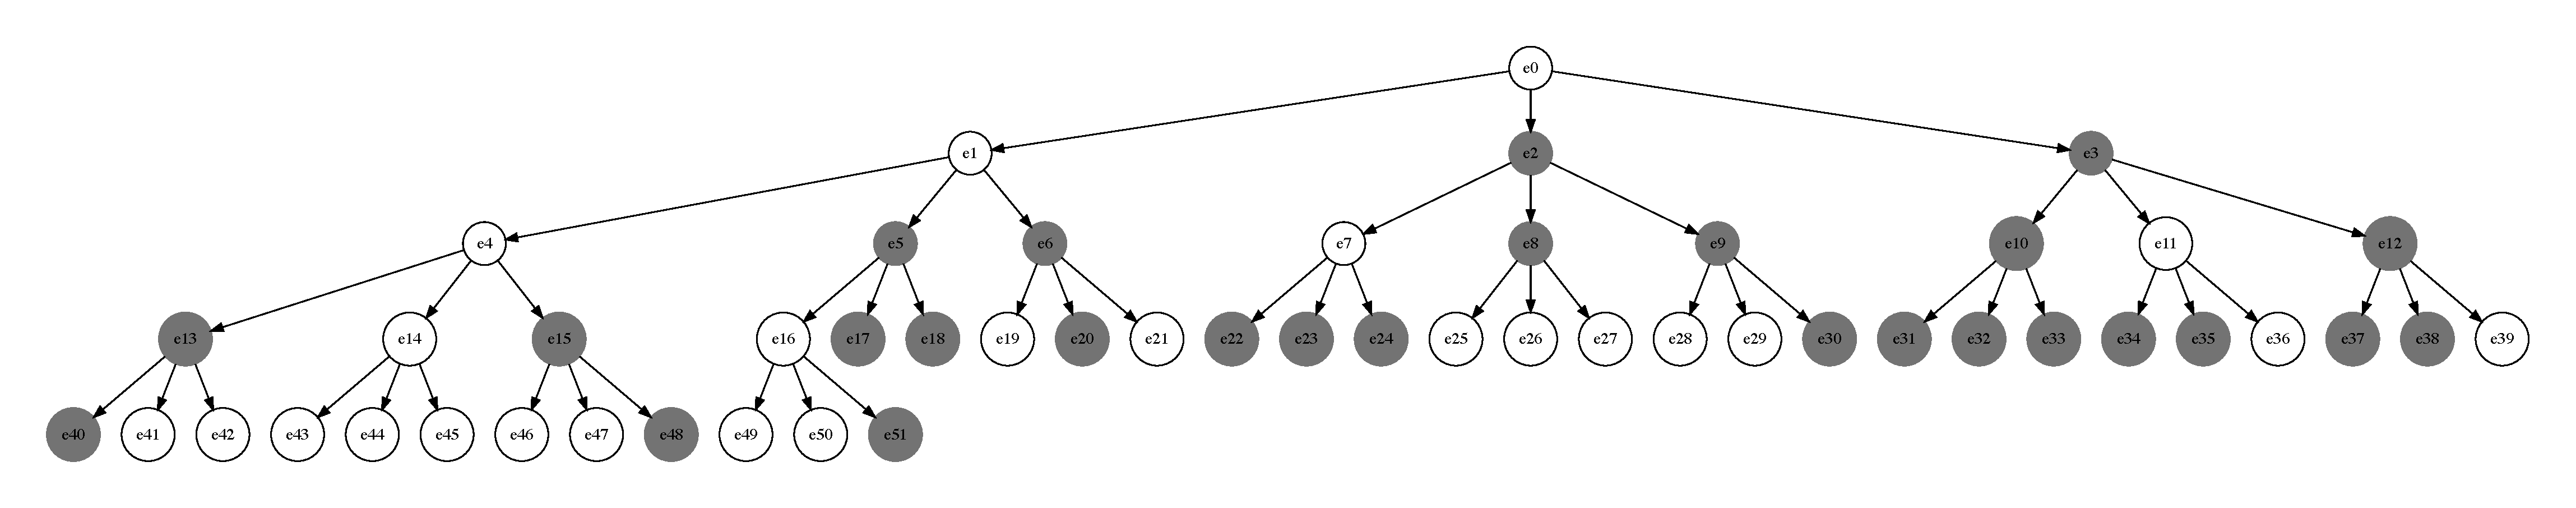
\includegraphics[width=\textwidth]{figs/Uni-hierachy.pdf}
  \end{minipage}
\end{figure}

For each employee, we use the generative model of Figure~\ref{fig:BN} to draw assignments for all the random variables. We assume that only $40\%$ of employees are qualified for promotion and regardless of their labels, employees submit only $60\%$ of their opinions. In addition, due to various personal and environmental factors, only $60\%$ of high quality employees perform well while $10\%$ of low quality employees also perform well regardless of their labels. Note that these numbers are not specific and just chosen for the framework to serve as a representative setting and a proof of concept. The conditional probability table for the opinion variable $O$ is parameterized by four values $(\theta_1, \theta_2, \theta_3, \theta_4)$ which together determine the degree of discrimination against the protected group. Since other parameters in the Bayesian network did not have a direct effect on the degree of discrimination, we fixed them to arbitrary values. 

The results presented in this section are based on an organization hierarchy  with $100$ employees where $k=5$. However, the results of the framework are not sensitive to the settings as we test the framework with various organization sizes ranging from $50$ to $500$ employees and various degree for $k$ ranging from $3$ to $10$. We generated seven datasets given the organization hierarchy using different values for the $\theta$ parameters: $(0.0,1.0,0.0,0.0)$, $(0.33,1.0,0.0,0.0)$, $(0.66,1.0,0.0,0.0)$, $(1.0,1.0,0.0,0.0)$, $(1.0,1.0,0.0,0.33)$, $(1.0,1.0,0.0,0.66)$, $(1.0,1.0,0.0,1.0)$. 
 
In the first three settings the discrimination originates from negative opinions towards qualified outgroup employees. The first setup is an extreme case where the opinion towards outgroup employees is always negative. The discrimination in the last three settings originates from positive opinions towards unqualified ingroup employees. The last setup is an extreme case where the opinion towards ingroup employees is always positive. The fourth setup represent unbiased opinions where employees are treated similarly based on their qualification. 

\paragraph{MAP Inference} We use the model presented in Table~\ref{tab:pslmodel} for MAP inference in PSL and FairPSL (recall that in FairPSL, the $\delta$-fairness constraints corresponding to one of the fairness measures are also added to the model). The observed atoms are $\textit{Manager(m,e)}$, $\textit{PositiveReview(e1,e2)}$ and labels of all employees. The truth values for all other atoms are obtained via MAP inference. We use the truth values obtained for the decision atoms $\textit{ToPromote(e)}$ to compute the fairness measures. We defined the discriminative pattern, and the protected and unprotected groups of this problem in Section~\ref{sec:formulation}.


\subsection{Evaluation results}

\begin{figure}
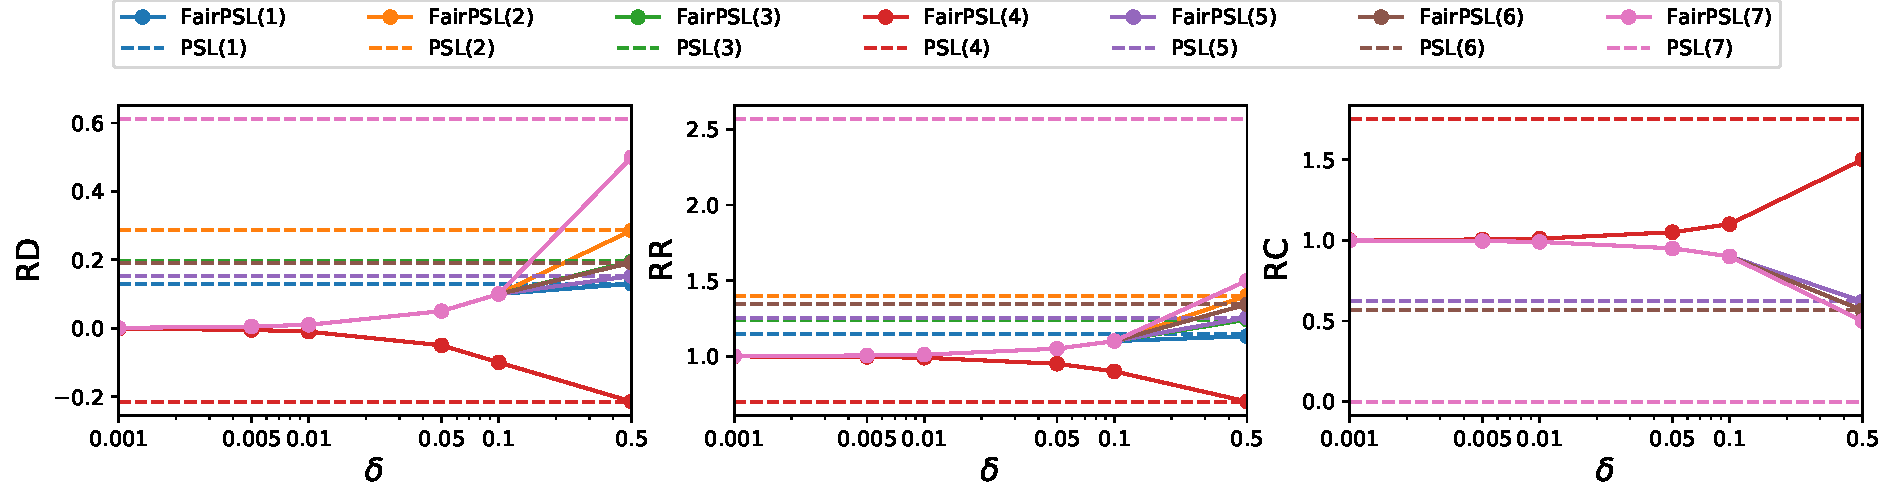
\includegraphics[width=1\linewidth]{figs/results_vis_uni_params.pdf}
\caption{\small Fairness score of predictions obtained by MAP inference of PSL and FairPSL, according to the fairness measures \emph{RD}, \emph{RR}, and \emph{RC}. The labels of datasets are mentioned with parenthesis next to the inference method. The FairPSL values of each measure are obtained by adding the $\delta$-fairness constraint of that measure.\label{fig:results}
}  
\end{figure}

To answer \textbf{Q1}, we run the MAP inference algorithm of PSL and FairPSL on seven synthetic datasets. 
We run the MAP inference of FairPSL multiple times on each dataset: For each of the three fairness measures, we add the corresponding $\delta$-fairness constraint with five thresholds $\{0.001, 0.005, 0.01, 0.05, 0.1, 0.5\}$.

Figure~\ref{fig:results} shows the fairness score of predictions in terms of the three fairness measures. As expected, tighter $\delta$-fairness constraints lead to better scores. Note that the best possible score according to RD is 0, as it computes a difference. Since RR and RC compute ratios, the best possible score according to these measures is 1. In our experiments, with any of these measures, taking $\delta = 0.001$ pushes the score of predictions to its limit.  

The $\delta$-fairness constraints modify the optimization problem of MAP inference by reducing the feasible region to solutions that conform with fairness guarantees. Research question \textbf{Q2} is concerned with the effect of this reduction on the accuracy of predictions. Note that decision quality is the same as the accuracy of predictions. To answer this question, we compare the inferred values for the decision atoms \textit{ToPromote(e)} against their actual values. These values are extracted from the known values of \textit{IsQualified(e)} according to rules 11 and 12 in Table~\ref{tab:pslmodel}. Figure~\ref{fig:accuracy} shows the area under the curve of the receiver operating characteristic~(AUC) of predicting the decision variable in three groups, namely the protected group, the unprotected group (i.e., promotion of the employees who have in-group managers), and all employees. By doing so, we make sure that our fairness constraints do not propagate bias towards either of the populations. Since the results of FairPSL with $\delta$-fairness constraints RR and RC are very similar to the results of RD, we only report the latter here.


\begin{figure}
    \centering
    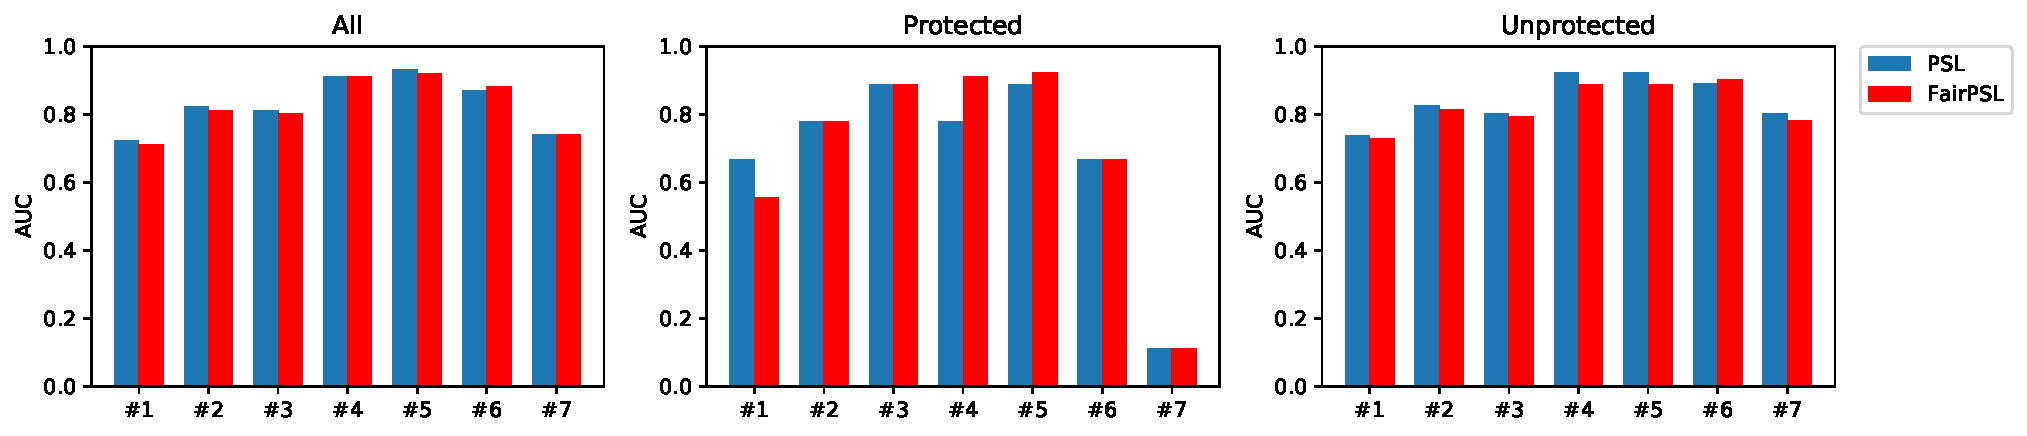
\includegraphics[width=\textwidth]{figs/roc.pdf}
    \caption{\small AUC score of predictions for truth values of unknown atoms \textit{ToPromote(e)} using MAP inference of PSL and FairPSL with $\delta$-fairness constraints $RD$ with $\delta=0.001$.}
    \label{fig:accuracy}
\end{figure}

According to Figure~\ref{fig:accuracy}, the results of both PSL and FairPSL in all seven datasets are close to each other. Note that although fairness may impose a cost in terms of overall accuracy, FairPSL often improves the accuracy of the protected class. Sometimes the overall predictions of FairPSL are even slightly better than PSL (e.g., dataset 6 and 7). As expected, the accuracy of the fourth setting where the opinions are unbiased are similar in both PSL and FairPSL. We observe that prediction of MAP inference for both FairPSL and PSL are similar, thus, in these settings at least, FairPSL guarantees fairness without hurting accuracy. Further investigation is required on the effect of the various ranges of discrimination (i.e., $\theta_1$, $\theta_2$, $\theta_3$, $\theta_4$) on the prediction results of FairPSL.



We also generate various types of organizations in which labels are not uniformly distributed, e.g., one population only occurs at the bottom levels of an organization. While we did not observe any differences in the behavior of our method with respect to accuracy and fairness measure, we found that the degree of discrimination is higher in such organizations. Further investigations on the structure of an organization on discrimination is an interesting direction for future research. 

\section{Conclusion and Future Directions}
\label{sec:conclusion}
Many applications of AI and machine learning affect peoples' lives in important ways. While there is a growing body of work on fairness in AI and ML, it assumes an individualistic notion of fairness.   In this paper, we have proposed a general framework for relational fairness which includes both a rich language for defining discrimination patterns and an efficient algorithm for performing inference subject to fairness constraints. We show our approach enforces fairness guarantees while preserving the accuracy of the predictions. 

There are many avenues for expanding on this work. For example, here we assumed that the discriminative pattern is given, however an automatic mechanism to extract discriminatory situations hidden in a large amount of decision records is an important and required task. Discrimination discovery has been studied for attribute-based fairness~\cite{pedreschi2013discovery}. An interesting next step is discrimination pattern discovery in relational data.

\section*{Acknowledgements}
This work is supported by the National Science Foundation under Grant Numbers CCF-1740850 and IIS-1703331. Golnoosh Farnadi and Behrouz Babaki are  supported by postdoctoral scholarships from IVADO through the Canada First Research Excellence Fund (CFREF) grant.

\begin{thebibliography}{10}
\itemsep=1pt 
\begin{small}

\bibitem{EUlaw}
European union legislation. (a) racial equality directive, 2000; (b) employment
  equality directive, 2000; (c) gender employment directive, 2006; (d) equal
  treatment directive (proposal), 2008.

\bibitem{UKlaw}
{UK} legislation. (a) sex discrimination act, 1975, (b) race relation act,
  1976.

\bibitem{USlaw}
United nations legislation. (a) universal declaration of human rights, 1948,
  (c) convention on the elimination of all forms of racial discrimination,
  1966, (d) convention on the elimination of all forms of discrimination
  against women, 1979.

\bibitem{alshukaili:iswc16}
Duhai Alshukaili, Alvaro A.~A. Fernandes, and Norman~W. Paton.
\newblock Structuring linked data search results using probabilistic soft
  logic.
\newblock In {\em International Semantic Web Conference {(1)}}, volume 9981 of
  {\em Lecture Notes in Computer Science}, pages 3--19, 2016.

\bibitem{bach:jmlr17}
Stephen~H. Bach, Matthias Broecheler, Bert Huang, and Lise Getoor.
\newblock Hinge-loss markov random fields and probabilistic soft logic.
\newblock {\em Journal of Machine Learning Research}, 18:109:1--109:67, 2017.

\bibitem{barocas2016big2}
Solon Barocas and Andrew~D Selbst.
\newblock Big data's disparate impact.
\newblock {\em California Law Review}, 104:671, 2016.

\bibitem{boyd2014networked}
Danah Boyd, Karen Levy, and Alice Marwick.
\newblock The networked nature of algorithmic discrimination.
\newblock In {\em Data and discrimination: Collected essays}, pages 53--57.
  2014.

\bibitem{brewer1979group}
Marilynn~B Brewer.
\newblock In-group bias in the minimal intergroup situation: A
  cognitive-motivational analysis.
\newblock {\em Psychological bulletin}, 86(2):307, 1979.

\bibitem{brewer2007social}
Marilynn~B Brewer.
\newblock The social psychology of intergroup relations: Social categorization,
  ingroup bias, and outgroup prejudice.
\newblock {\em Social Psychology: Handbook of Basic Principles}, 2007.

\bibitem{chouldechova2017fair2}
Alexandra Chouldechova.
\newblock Fair prediction with disparate impact: {A} study of bias in
  recidivism prediction instruments.
\newblock {\em CoRR}, abs/1703.00056, 2017.

\bibitem{dwork2012fairness3}
Cynthia Dwork, Moritz Hardt, Toniann Pitassi, Omer Reingold, and Richard~S.
  Zemel.
\newblock Fairness through awareness.
\newblock In {\em {ITCS}}, pages 214--226. {ACM}, 2012.

\bibitem{ebrahimi:emnlp16}
Javid Ebrahimi, Dejing Dou, and Daniel Lowd.
\newblock Weakly supervised tweet stance classification by relational
  bootstrapping.
\newblock In {\em {EMNLP}}, pages 1012--1017. The Association for Computational
  Linguistics, 2016.

\bibitem{farnadi2018fairness}
Golnoosh Farnadi, Behrouz Babaki, and Lise Getoor.
\newblock Fairness in relational domains.
\newblock In {\em AAAI/ACM Conference on AI, Ethics, and Society (AIES)}, pages
  108--114. ACM, 2018.

\bibitem{feldman2015certifying2}
Michael Feldman, Sorelle~A. Friedler, John Moeller, Carlos Scheidegger, and
  Suresh Venkatasubramanian.
\newblock Certifying and removing disparate impact.
\newblock In {\em {KDD}}, pages 259--268. {ACM}, 2015.

\bibitem{getoor2007introduction}
Lise Getoor and Ben Taskar.
\newblock {\em {Introduction to Statistical Relational Learning}}.
\newblock MIT press Cambridge, 2007.

\bibitem{hardt2016equality3}
Moritz Hardt, Eric Price, and Nati Srebro.
\newblock Equality of opportunity in supervised learning.
\newblock In {\em {NIPS}}, pages 3315--3323, 2016.

\bibitem{kamishima2011fairness}
Toshihiro Kamishima, Shotaro Akaho, and Jun Sakuma.
\newblock Fairness-aware learning through regularization approach.
\newblock In {\em ICDMW}, pages 643--650. {IEEE} Computer Society, 2011.

\bibitem{kouki:recsys15}
Pigi Kouki, Shobeir Fakhraei, James~R. Foulds, Magdalini Eirinaki, and Lise
  Getoor.
\newblock Hyper: {A} flexible and extensible probabilistic framework for hybrid
  recommender systems.
\newblock In {\em RecSys}, pages 99--106. {ACM}, 2015.

\bibitem{counterfactualfairness}
Matt~J. Kusner, Joshua~R. Loftus, Chris Russell, and Ricardo Silva.
\newblock Counterfactual fairness.
\newblock In {\em {NIPS}}, pages 4069--4079, 2017.

\bibitem{Pedreschi:2012}
Dino Pedreschi, Salvatore Ruggieri, and Franco Turini.
\newblock A study of top-k measures for discrimination discovery.
\newblock In {\em {SAC}}, pages 126--131. {ACM}, 2012.

\bibitem{pedreschi2013discovery}
Dino Pedreschi, Salvatore Ruggieri, and Franco Turini.
\newblock The discovery of discrimination.
\newblock In {\em Discrimination and Privacy in the Information Society},
  volume~3 of {\em Studies in Applied Philosophy, Epistemology and Rational
  Ethics}, pages 91--108. Springer, 2013.

\bibitem{ridgeway2004unpacking}
Cecilia~L Ridgeway and Shelley~J Correll.
\newblock Unpacking the gender system: A theoretical perspective on gender
  beliefs and social relations.
\newblock {\em Gender \& society}, 18(4):510--531, 2004.

\bibitem{sridhar:bioinformatics16}
Dhanya Sridhar, Shobeir Fakhraei, and Lise Getoor.
\newblock A probabilistic approach for collective similarity-based drug-drug
  interaction prediction.
\newblock {\em Bioinformatics}, 32(20):3175--3182, 2016.

\bibitem{verma2018fairness2}
Sahil Verma and Julia Rubin.
\newblock Fairness definitions explained.
\newblock In {\em 2018 IEEE/ACM International Workshop on Software Fairness
  (FairWare)}, pages 1--7. IEEE, 2018.

\bibitem{west2014exploiting}
Robert West, Hristo~S. Paskov, Jure Leskovec, and Christopher Potts.
\newblock Exploiting social network structure for person-to-person sentiment
  analysis.
\newblock {\em {TACL}}, 2:297--310, 2014.

\bibitem{zafar2017parity}
Muhammad~Bilal Zafar, Isabel Valera, Manuel Gomez{-}Rodriguez, Krishna~P.
  Gummadi, and Adrian Weller.
\newblock From parity to preference-based notions of fairness in
  classification.
\newblock In {\em {NIPS}}, pages 228--238, 2017.

\bibitem{zemel2013learning}
Richard~S. Zemel, Yu~Wu, Kevin Swersky, Toniann Pitassi, and Cynthia Dwork.
\newblock Learning fair representations.
\newblock In {\em {ICML} {(3)}}, volume~28 of {\em {JMLR} Workshop and
  Conference Proceedings}, pages 325--333. JMLR.org, 2013.

\end{small}
\end{thebibliography}

\end{document}

\end{article}



\end{articlesection}

% put the news items below- there can be multiple news sections
% each with its own title
% news will usually have an author as well as a title, 
% e.g. TCDE elections
% news articles are in the same format as letters
% typically, news articles will be stored in a directory called "news"

%\begin{newssection}{News headline}

% insert news items here; news will typically have authors
% see the Sept. 2018 issue for an example

%\begin{news}{news item title}
%{author name}{author affiliation}
%\input{news/news-article.tex}
%\end{news}
%
%\newpage


%\end{newssection}



\begin{callsection}

%  This section will be empty for your version
%
%  Calls for papers section.  Use the callsection environment.
%  Each call for papers is contained in an call environment, where the single 
%  required options to \begin{call} is the name of the conference.
% typically calls are stored in a "calls" directory
%
%\begin{call}{name of conference}
%\centerline{\includegraphics[width=\textwidth, bb= 0 0 590 760]{calls/conference-name.pdf}}
%\end{call}
%\begin{call}{ICDE 2019 Conference}
%\centerline{\includegraphics[width=\textwidth, bb= 0 0 610 790] {../Dec-2018/calls/icde19.pdf}} 
%\centerline{\includegraphics[width=\textwidth, bb= 0 0 590 760] {calls/icde19.pdf}}
%\end{call}
\begin{call}{TCDE Membership Form}
%\centerline{\includegraphics[width=\textwidth, bb= 0 0 610 790]
\centerline{
\includegraphics[width=\textwidth, bb= 0 0 590 760] {../Dec-2018/calls/tcde.pdf}}
\end{call}

\end{callsection}

\end{bulletin}
\end{document}
